\documentclass[runningheads]{llncs}

%% Save the class definition of \subparagraph
\let\llncssubparagraph\subparagraph
%% Provide a definition to \subparagraph to keep titlesec happy
\let\subparagraph\paragraph
%% Load titlesec
\usepackage[compact]{titlesec}
%% Revert \subparagraph to the llncs definition
\let\subparagraph\llncssubparagraph

\usepackage{amssymb,amsmath}
\usepackage{latexsym}
\usepackage{graphicx}
\usepackage{textcomp}
\usepackage{txfonts} %% for various points-to symbols. use pxfonts for 5-tip stars
\usepackage{verbatim} %% for comment environment
\usepackage{xspace} %% for comment environment
\usepackage{cancel} % for crossing Owns 
\usepackage{mathpartir}
\usepackage{soul}
\usepackage{xcolor}
\usepackage{multirow}
\usepackage{stmaryrd} 
% % sorting citation
\usepackage{url}
\usepackage{float} 
\usepackage{framed}
\usepackage{hyperref}
% Fonts
\usepackage{bbm}
\usepackage{alltt}
\usepackage{verbdef}
\usepackage{titlesec}
\usepackage{parskip}
\usepackage{wrapfig}
\usepackage{cite}

\setlength{\intextsep}{5pt}%

\setlength{\parindent}{0.15in}
\setlength{\topsep}{0cm}
\setlength{\parskip}{0pt}
\titlespacing*{\section}{0pt}{*1}{*1}
\titlespacing*{\subsection}{0pt}{*0.7}{*0.5}
\titlespacing*{\paragraph}{0pt}{*0.5}{*0.5}
\renewcommand{\figurename}{Fig.}

\hyphenation{time-stamp time-stamps}

%%%%%%%%%%%%%%%%%%%%%%%%%%%%%%%%%%%%%%%%%%%%%%%%%%%%%%%%%%%%%%%%%%%%%%
% Floats

\renewcommand{\textfraction}{0.1}
\renewcommand{\topfraction}{0.95}
\renewcommand{\dbltopfraction}{0.95}
\renewcommand{\floatpagefraction}{0.9}
\renewcommand{\dblfloatpagefraction}{0.9}

\setlength{\floatsep}{16pt plus 4pt minus 4pt}
\setlength{\textfloatsep}{16pt plus 4pt minus 4pt}

\floatstyle{ruled} 
\restylefloat{figure}  

% reducing the sf math fonts somewhat
\usepackage[T1]{fontenc}

\DeclareFontFamily{OML}{zavm}{\skewchar\font=127 }
\DeclareFontShape{OML}{zavm}{m}{n}{<-> s*[.80] zavmr7t}{}
\DeclareFontShape{OML}{zavm}{b}{n}{<-> s*[.80] zavmb7t}{}
\DeclareFontShape{OML}{zavm}{m}{it}{<-> s*[.80] zavmri7m}{}
\DeclareFontShape{OML}{zavm}{b}{it}{<-> s*[.80] zavmbi7m}{}
\DeclareFontShape{OML}{zavm}{m}{sl}{<->ssub * zavm/m/it}{}
\DeclareFontShape{OML}{zavm}{bx}{it}{<->ssub * zavm/b/it}{}
\DeclareFontShape{OML}{zavm}{b}{sl}{<->ssub * zavm/b/it}{}
\DeclareFontShape{OML}{zavm}{bx}{sl}{<->ssub * zavm/b/sl}{}
\DeclareMathAlphabet{\mathsf}{OML}{zavm}{m}{n} % not `n'

% Figures should be boxed
%    *** Uncomment the next two lines to box the floats *** 
% \floatstyle{boxed}
% \restylefloat{figure}

% Keep footnotes on one page
\interfootnotelinepenalty=10000 

%%%%%%%%%%%%%%%%%%%%%%%%%%%%%%%%%%%%%%%%%%%%%%%%%%%%%%%%%%%%%%%%%%%%%%
% Compiling two paper versions
%%%%%%%%%%%%%%%%%%%%%%%%%%%%%%%%%%%%%%%%%%%%%%%%%%%%%%%%%%%%%%%%%%%%%%

\newcommand{\ifext}[2]{\ifdefined\extflag{#1}\else{#2}\fi}
\newcommand{\ifcomm}[1]{\ifdefined\extcomm{#1}\else{}\fi}

\newcommand{\mute}[1]{\ifdefined\draftflag{#1} \else{} \fi}
%\newcommand{\mute}[1]{}

\usepackage{skull}

\newcounter{ToDos}
\newcounter{WarnCounts}
\newcommand{\decorateWC}{
  \stepcounter{WarnCounts}
  \marginpar{\textcolor{red}{$\skull\ \theWarnCounts$}}}

\newcommand{\decorateTD}{
  \stepcounter{ToDos}
  \marginpar{\textcolor{red}{$\textbf{TO DO}_{\#\ \theToDos}$}}}


% Skeleton for remark comments
% 1: Name, 2: Color, 3:Comment
\newcommand{\signedComment}[3]
           {\mute{\textcolor{#2}{(#1: {#3})}\decorateWC}}

% remarks
\newcommand{\todo}[1]{\mute{\textcolor{red}{(TO DO:{#1})}\decorateTD}}

\newcommand{\is}[1]{\signedComment{Ilya}{blue}{#1}}
\newcommand{\an}[1]{\signedComment{Aleks}{red}{#1}}
\newcommand{\ab}[1]{\signedComment{AB}{red}{#1}}
\newcommand{\gad}[1]{\signedComment{GAD}{red}{#1}}

\newcommand{\highlight}[1]
           {\ifdefined\draftflag{{\textcolor{red}{#1}}} \else{#1} \fi}

\newenvironment{draft}
           {\ifdefined\draftflag \par\color{red} \else \comment \fi}
           {\ifdefined\draftflag \decorateWC\par \else \endcomment \fi}
           
% useful macros
\newcommand{\asgn}{\leftarrow}
\newcommand{\code}[1]{\lstinline[basicstyle=\small\ttfamily]{#1}}
\newcommand{\ccode}[1]{\lstinline[basicstyle=\footnotesize\ttfamily]{#1}}
\newcommand{\cccode}[1]{\lstinline[basicstyle=\scriptsize\ttfamily]{#1}} 
\newcommand{\Code}[1]{\code{#1}}
\newcommand{\etc}{\emph{etc}}
\newcommand{\ie}{\emph{i.e.}\xspace}
\newcommand{\id}{\emph{Id.}\xspace}
\newcommand{\eg}{\emph{e.g.}\xspace}
\newcommand{\vs}{\emph{vs.}\xspace}
\newcommand{\etal}{\emph{et~al.}\xspace}
\newcommand{\adhoc}{\emph{ad~hoc}\xspace}
\newcommand{\viz}{\emph{viz.}\xspace}
\newcommand{\dom}[1]{\mathsf{dom}(#1)}
\newcommand{\aka}{\textit{a.k.a.}\xspace}
\newcommand{\cf}{\textit{cf.}\xspace}
\newcommand{\wrt}{{wrt.}\xspace}
\newcommand{\Iff}{{iff}\xspace}
\newcommand{\loef}{L\"{o}f}
\newcommand{\sep}{\textasteriskcentered}
\newcommand{\res}{\mathsf{res}}
\newcommand{\bal}{\mathit{bal}} 
\newcommand{\ret}{\mathsf{ret}} 
\newcommand{\fix}{\mathsf{fix}} 
\newcommand{\Unit}{\mathsf{Unit}}  
\newcommand{\ic}{\mathcal{I}}
\newcommand{\Ic}[2]{\ic~{#1}~{#2}}
\newcommand{\hide}{\mathsf{hide}}  
\newcommand{\last}{\mathsf{last}}  

%specs
\newcommand{\specK}[1]{\ensuremath{\textcolor{blue}{#1}}}
\newcommand{\comm}[1]{\ensuremath{\textcolor{gray}{\esc{/\!/}~{#1}}}}
\newcommand{\spec}[1]{\specK{\left\{{#1}\right\}}}
\newcommand{\specQ}[4]{[#1 , #2 , #3] \, #4}%\specQ{mL}{gL}{gE}{p}
\newcommand{\drspec}[1]{\specK{\langle{#1}\rangle}}
\newcommand{\sspec}[1]{\specK{\{{#1}\}}}
\newcommand*{\backin}{\rotatebox[origin=c]{-180}{$\in$}}%

%actions
\newcommand{\act}[1]{\textsf{\small{#1}}}
\newcommand{\aux}[1]{\textit{#1}}
\newcommand{\Aux}[1]{\(\mathit{\small{#1}}\)}
\newcommand{\Num}[1]{{\text{{\scriptsize{#1}}}}}
\newcommand{\esc}[1]{\text{\texttt{\small{#1}}}}
\newcommand{\kw}[1]{\text{\textbf{#1}}}
\newcommand{\tp}[1]{\text{\textsf{#1}}}
\newcommand{\Asgn}{\leftarrow} 

%PCMs
\newcommand{\dotcup}{\ensuremath{\mathaccent\cdot\cup}}
\newcommand{\pcmS}{\mathbb{U}}
\newcommand{\pcmF}{\bullet}
\newcommand{\join}{\pcmF}
\newcommand{\jjoin}[1]{\ensuremath{\bigodot}_{#1=1}^n} 
\newcommand{\pcmU}{\mathbbm{1}}

% Pretty table
\newcommand{\cmark}{\ding{52}}%
\newcommand{\xmark}{\ding{55}}%
\newcommand*\rot{\rotatebox{32}} 
\newcommand{\yep}{\ding{51}}
\newcommand{\yepl}{$\text{\ding{51}}_{\!\!L}$}  
\newcommand{\yepa}{$\text{\ding{51}}_{\!\!L}$}  
\newcommand{\intab}[1]{({\sffamily{\small{#1}}})}

% Concurroids
\newcommand{\acon}{\mathcal{A}}
\newcommand{\econ}{\mathcal{E}}
\newcommand{\ucon}{\mathcal{U}}
\newcommand{\rcon}{\mathcal{R}}
\newcommand{\ccon}{\mathcal{C}}
\newcommand{\vcon}{\mathcal{V}}
\newcommand{\wcon}{\mathcal{W}}
\newcommand{\privcon}{\mathcal{P}}
\newcommand{\pscon}{\mathcal{S}}
\newcommand{\tbcon}{\mathcal{T}}
\newcommand{\fccon}{\mathcal{F}}
\newcommand{\lcon}{\mathcal{L}}
\newcommand{\alloccon}{\mathcal{A}}
\newcommand{\jayanticon}{\mathcal{J}}

%Getters
\newcommand{\lcl}{{\mathsf{s}}}%L
\newcommand{\env}{{\mathsf{o}}}%E
\newcommand{\joint}{{\mathsf{j}}}%E

\newcommand{\selfsub}{\mathsf{s}}
\newcommand{\othersub}{\mathsf{o}}
\newcommand{\jointsub}{\mathsf{j}}

\newcommand{\hist}{\chi} 
\newcommand{\histS}{\hist_{\, \selfsub}}
\newcommand{\histO}{\hist_{\, \othersub}}
\newcommand{\histJ}{\hist_{\, \jointsub}}
\newcommand{\hempty}{\emptyset}
\def\envsteps{\rightarrow^{*}_{\epsilon}}

\newcommand{\heap}{h} 
\newcommand{\heapS}{\heap_{\, \selfsub}}
\newcommand{\heapSP}{\heap_{\, \selfsub}'}

% Jayanti's Snapshot getters

\def\ordlist{\sigma}
\newcommand{\E}{\tau}
\newcommand{\C}{\kappa}


% Jayanti's Snapshot Orders
\newcommand{\tleq}{\mathrel{\leq_\ordlist}}
\newcommand{\tle}{\mathrel{<_\ordlist}}

\newcommand{\stableorder}{\Omega}
\newcommand{\prefix}[1]{-\,{\tleq}\,#1}

% Primed getters

\def\ordlistP{\sigma'}
\newcommand{\stableorderP}{\stableorder'}
\newcommand{\prefixP}[1]{(\mathrel{\tleqP}#1)}
\newcommand{\tleP}{\mathrel{<_\ordlistP}}
\newcommand{\tleqP}{\mathrel{\leq_\ordlistP}}
\newcommand{\EP}{\tau'}
\newcommand{\CP}{\kappa'}
\newcommand{\histP}{\chi'} 
\newcommand{\histSP}{\hist_{\, \selfsub}'}
\newcommand{\histOP}{\hist_{\, \othersub}'}
\newcommand{\histJP}{\hist_{\, \jointsub}'}

\newcommand{\wxP}{W_\x'}
\newcommand{\wyP}{W_\y'}
\newcommand{\wppP}{W_p'}

\newcommand{\jge}{\mathrel{>_\ordlist}}

\def\lgVy{\ensuremath{\mathsf{lastGY}}}


%% Writer and scanner states.

\newcommand{\wInit}{\mathsf{W_{Off}}}
\newcommand{\wWrite}{\mathsf{New}}
\newcommand{\wDirty}{\mathsf{Fwd}}
\newcommand{\wClean}{\mathsf{Done}}

\newcommand{\sOn}{\mathsf{S_{On}}}
\newcommand{\sOff}{\mathsf{S_{Off}}}

%mapsto stuff
\makeatletter
\newcommand{\oset}[3][0ex]{%
  \mathrel{\mathop{#3}\limits^{
    \vbox to#1{\kern-3\ex@
    \hbox{$\scriptstyle#2$}\vss}}}}
\makeatother

\makeatletter
\newcommand{\ojset}[3][0ex]{%
  \mathrel{\mathop{#3}\limits^{
    \vbox to#1{\kern-5\ex@
    \hbox{$\scriptstyle#2$}\vss}}}}
\makeatother

\newcommand{\jpts}{\mathrel{\ojset{j}{\mapsto}}}
\newcommand{\spts}{\mathrel{\oset{s}{\mapsto}}}
\newcommand{\opts}{\mathrel{\oset{o}{\mapsto}}}
\newcommand{\qcl}{\mathsf{cn}}

\newcommand{\hunion}{\mathbin{\dotcup}} 
\newcommand{\Hunion}[1]{\mathbin{\Dotcup{#1}}}

%% operators

\newcommand{\eqdef}{\mathrel{\:\widehat{=}\:}}
\newcommand{\hpts}{\mapsto}
\newcommand{\ldot}{\mathord{.}\,}

%% \newcommand{\aand}{,}
%% \newcommand{\oor}{\vee}
%% \newcommand{\nnot}{\neg}
%% \newcommand{\eqq}{\mathrel{\mbox{\tt==}}}
%% \newcommand{\neqq}{\mathrel{\mbox{\tt!=}}}
%% \newcommand{\andb}{\mathrel{\small\mbox{\&\&}}}
%% \newcommand{\orb}{\mathrel{\mbox{\tt{|\!|}}}}
%% \newcommand{\evar}[1]{?#1}
%% \newcommand{\zig}{\triangleleft}
%% \newcommand{\zag}{\triangleright}
%% \newcommand{\set}[1]{\left\{#1\right\}}
%% \newcommand{\tauflip}{\mathsf{flip\_trans}}
%% \newcommand{\tauadd}{\mathsf{add2\_trans}}
%% \newcommand{\tfr}[2]{{\text{fresh}^{#2}_{#1}}}

%% % more invariants
%% \newcommand{\tapprox}{\mathsf{ResInterf}}
%% \newcommand{\happrox}{\mathsf{ResPast}}
%% %\newcommand{\sapprox}{\mathsf{ResState}}
%% \newcommand{\bapprox}{\mathsf{ValuesMono}}
%% \newcommand{\strapprox}{\mathsf{IncResult}}
%% \newcommand{\Thisz}{\mathsf{this}}
%% \newcommand{\This}[1]{\Thisz~{#1}}

%% \newcommand{\hvalid}{\mathsf{Valid}}
%% \newcommand{\eqqc}{e_{\mathit{qqc}}}
%% \newcommand{\eqc}{e_{\mathit{qc}}}

%% \newcommand{\pending}{{m_\joint}} 
%% \newcommand{\offers}{h}
%% \newcommand{\twin}[1]{\bar{#1}}
%% \newcommand{\mygathjyer}[1]{|\!|{#1}|\!|}

%% \definecolor{shadecolor}{gray}{1.00}
%% \definecolor{ddarkgray}{gray}{0.75}
%% \definecolor{darkgray}{gray}{0.30}
%% \definecolor{light-gray}{gray}{0.87}
%% \newcommand{\whitebox}[1]{\colorbox{white}{#1}}
%% \newcommand{\graybox}[1]{\colorbox{light-gray}{#1}}
%% \newcommand{\darkgraybox}[1]{\colorbox{ddarkgray}{#1}}
%% \newcommand{\gbm}[1]{\graybox{${#1}$}}



%%% Snapshots paper related
%%%

\def\FF{\mathsf{False}}
\def\TT{\mathsf{True}}


%%% Specs
\newcommand{\tsPre}[1]{\ensuremath{{\textcolor{blue}{#1}}}}
\newcommand{\tsPos}[1]{\ensuremath{\textcolor{blue}{#1}}}
\newcommand{\logvar}[1]{\ensuremath{\textcolor{blue}{[#1].}}}

\newcommand{\var}[1]{\mathit{#1}} 
\newcommand{\num}[1]{{\text{{\scriptsize{#1}}}}}


\newcommand{\hfilter}{\mathrel{\downarrow}}

%% \newcommand{\cevX}[2]{\cev{#1}_{#2}}

%% \makeatletter
%% \DeclareRobustCommand{\cev}[1]{%
%%   \mathpalette\do@cev{#1}%
%% }

%% \newcommand{\do@cev}[2]{%
%%   \fix@cev{#1}{+}%
%%   \reflectbox{$\m@th#1\vec{\reflectbox{$\fix@cev{#1}{-}\m@th#1#2\fix@cev{#1}{+}$}}$}%
%%   \fix@cev{#1}{-}%
%% }
%% \newcommand{\fix@cev}[2]{%
%%   \ifx#1\displaystyle
%%     \mkern#23mu
%%   \else
%%     \ifx#1\textstyle
%%       \mkern#23mu
%%     \else
%%       \ifx#1\scriptstyle
%%         \mkern#22mu
%%       \else
%%         \mkern#22mu
%%       \fi
%%     \fi
%%   \fi
%% }


\def\GYR{{\mathbf{{g^{+}}{y^{?}}{r^{*}}}}}
\def\RZ{{\mathbf{{{(g | y)^{+}}}{r^{*}}}}}

%% \def\GYR{{\mathbf{{\color{OliveGreen}{G^{+}}}\bullet%
%%                    \color{YellowOrange}{Y^{?}}}\bullet%
%%                    \color{WildStrawberry}{R^{*}}}}



% code

\def\lat{\langle}
\def\rat{\rangle}
\def\tbnd{\Asgn}
\newcommand{\actwrite}[2]{{#1}\,{:=}\,{#2}}

%\def\altsubseteq{\mathbin{\subseteq}}

\newcounter{tags}

\newcommand{\mytitle}{Specifying and Verifying Concurrent
  Algorithms \\
with Histories and Subjectivity}
%\newcommand{\mytitle}{
%  Specifying and Verifying Fine-Grained Concurrent Algorithms \\{} 
%  using Histories and Subjectivity}
% \newcommand{\mytitle}{
%   Specifying Interference in Hoare-Style Logic for Concurrency}

\clubpenalty=10000 
\widowpenalty = 10000 

%%%%%%%%%%%%%%%%%%%%%%%%%%%%%%%%%%%%%%%%%%%%%%%%%%%%%%%%%%%%%%%%%%%%%%
% Floats

\begin{document} 

%\special{papersize=8.5in,11in}
\setlength{\pdfpageheight}{\paperheight}
\setlength{\pdfpagewidth}{\paperwidth}

% \subtitle{Extended version}
%\subtitle{\large{\color{red}\today}}

%

\author{Ilya Sergey \and 
  Aleksandar Nanevski \and
  Anindya Banerjee}

\institute{IMDEA Software Institute, Spain\\ 
\email{\{ilya.sergey, aleks.nanevski, anindya.banerjee\}@imdea.org}}

\title{\mytitle}

\maketitle 

\begin{abstract}

  We present a lightweight approach to Hoare-style specifications for
  fine-grained concurrency, based on a notion of \emph{time-stamped
    histories} that abstractly capture atomic changes in the program
  state.
% 
Our key observation is that histories form a \emph{partial commutative
  monoid}, a structure fundamental for representation of concurrent
resources.
%
This insight provides us with a unifying mechanism that allows us to
treat histories just like heaps in separation logic. For example, both
are subject to the same assertion logic and inference rules (\eg, the
frame rule). Moreover, the notion of ownership transfer, which usually
applies to heaps, has an equivalent in histories. It can be used to
formally represent helping---an important design pattern for
concurrent algorithms whereby one thread can execute code on behalf of
another.
%
Specifications in terms of histories naturally abstract away the
internal interference, so that sophisticated fine-grained algorithms
can be given the same specifications as their simplified
coarse-grained counterparts, making them equally convenient for
client-side reasoning.
% 
We illustrate our approach on a number of examples and validate all of
them in~Coq.
  
\end{abstract}

% \category{D.1.1}{Programming Techniques}{Applicative (Functional) Programming}
% %
% \category{F.3.2}{Logics and Meanings of Programs}{Semantics of
%  Programming Languages --- Program analysis, Operational semantics}

% do nothing

% \terms
% Languages, Theory, Verification

\section{Introduction}
\label{sec:intro}

For sequential programs and data structures, Hoare-style
specifications (or specs) in the form of pre- and postconditions are %uniformly
%accepted as 
a declarative way to express a program's behavior. For example, an
abstract specification of stack operations can be given as follows:
%
\[
\tag{\arabic{tags}}\refstepcounter{tags}\label{eq:seqstack-spec} 
{\small
\hspace{-5pt}
\begin{array}{r@{\ }c@{\ }l}
\spec{~s \hpts \mathit{xs}~} &\Cmd{push}{x} & \spec{~ s \hpts
  x::\mathit{xs}~}
\\[3pt]
\spec{~s \hpts \mathit{xs}~} & \Cmd{pop}{} &\spec{
\begin{array}{l}
  \res = \None \aand \mathit{xs} = \nil \aand s \hpts \nil \oor \hbox{}\\
  \res = \Some x \aand \exists \mathit{xs'},~\mathit{xs} = x ::\mathit{xs'} \aand
  s \hpts \mathit{xs'}
\end{array}
}
\end{array}
}
\]
% 
where $s$ is an ``abstract pointer'' to the data structure's logical
contents, and the logical variable $\mathit{xs}$ is universally
quantified over the spec.
%
The result $\res$ of $\cmd{pop}$ is either $\Some x$, if $x$ was on
the top of the stack, or $\None$ if the stack was empty.
%
The spec (\ref{eq:seqstack-spec}) is usually accepted as canonical for
stacks: it hides the details of method implementation, but exposes
what is important about the method behavior, so that a verification of
a stack \emph{client} does not need to explore the implementations of
$\cmd{push}$ and $\cmd{pop}$.

The situation is much more complicated in the case of concurrent data
structures. In the concurrent setting, the
spec~\eqref{eq:seqstack-spec} is of little use for implementations
with server-side locking, as the interference of the threads executing
concurrently may invalidate the assertions about the stack. For
example, a call to $\cmd{pop}$ may encounter an empty stack, and
decide to return $\None$, but by the time it returns, the stack may be
filled by the other threads, thus invalidating the postcondition of
$\cmd{pop}$ in~\eqref{eq:seqstack-spec}. To soundly reason about
concurrent data structures, one has to devise specs that are
\emph{stable} (\ie, invariant under interference), but this may
require trade-offs with respect to the specifications' expressivity
and precision for the client's needs.
% 

Reasoning about concurrent data structures is further complicated by
the fact that their implementations are often \emph{fine-grained}.
Striving for better performance, they avoid explicit locking, and
implement sophisticated synchronization patterns that deliberately
rely on interference.
% 
For reasoning purposes, however, it is desirable that the clients can
perceive such fine-grained implementations as if they were
\emph{coarse-grained}; that is, as if the effects of their methods
take place \emph{atomically}, at singular points in time.  The
standard correctness criteria of
\emph{linearizability}~\cite{Herlihy-WingTOPLAS90} establishes that a
fine-grained data structure implementation \emph{contextually refines}
a coarse-grained one~\cite{Filipovic-al:TCS10}. One can make use of a
refined, fine-grained, implementation for efficiency in programming,
but then soundly replace it with a more abstract coarse-grained
implementation to simplify the reasoning about clients.

% , 
% therefore
%taking advantage of a \emph{granularity abstraction}.

Semantically, one program linearizes to another if the
\emph{histories} of the first program (\ie, the sequence of actions it
executed) can be transformed, in a suitable sense, into the histories
of the second. Thus, histories are an essential ingredient in
specifying fine-grained concurrent data structures. However, while a
number of logical methods exist for establishing the linearizability
relation between two programs, for a class of data
structures~\cite{OHearn-al:PODC10,Elmas-al:TACAS10,Vafeiadis:PhD,Liang-Feng:PLDI13},
in general, it is a non-trivial property to prove and use. First, in a
setting that employs Hoare-style reasoning, showing that a
fine-grained structure refines a coarse-grained one is not an end in
itself. One still needs to ascribe a stable spec to the coarse-grained
version~\cite{Turon-al:ICFP13,Liang-Feng:PLDI13}.
%
Second, the standard notion of linearizability does not directly
account for modern programming features, such as ownership transfer of
state between threads, pointer aliasing, and higher-order
procedures. Theoretical extensions required to support these features
are a subject of active ongoing
research~\cite{Cerone-al:ICALP14,Gotsman-Yang:CONCUR12}.
%
Finally, being a relation on \emph{two} programs, deriving
linearizability by means of logical inference inherently requires a
\emph{relational program
  logic}~\cite{Turon-al:ICFP13,Liang-Feng:PLDI13}, even though the
spec one is ultimately interested in 
%(\eg,~\eqref{eq:stack-weak} for a concurrent stack) 
may be expressed using a Hoare triple that operates over a
\emph{single} program.

In this paper, we propose a novel method to specify and verify
fine-grained programs by directly reasoning about histories in the
specs of an elementary Hoare logic. We propose using
\emph{timestamped} histories, which carry information about the atomic
changes in the abstract state of the program, indexed by discrete
timestamps, and tracking the history of a program as a form of
auxiliary state.

While using histories in Hoare-style specs is a simple and natural
idea, and has been used
before~\cite{Bell-al:SAS10,Fu-al:CONCUR10,Gotsman-al:ESOP13}, in our
paper it comes with two additional novel observations.

First, timestamped histories are technically very similar to heaps, as
both satisfy the algebraic properties of a \emph{partial commutative
  monoid} (PCM). A PCM is a set $\pcmS$ with an associative and
commutative \emph{join} operation $\pcmF$ and unit element
$\pcmU$. Both heaps and histories (considered as sets of actions with
distinct timestamps, correspondingly) form a PCM with disjoint union
and empty heap/history as the unit. Also, a singleton history $t \hpts
a$ is similar to the singleton heap $x \hpts v$ containing only the
pointer $x$ with value $v$.
%
We emphasize the connection by using the same notation for~both.
%
The common PCM structure makes it possible to reuse for histories the
ideas and results developed for heaps in the work on separation
logic~\cite{Calcagno-al:LICS07}. In particular, in this paper, we make
both heaps and histories subject to the same assertion logic, the same
rules of inference (\eg, the frame rule), and thus the same style of
\emph{local reasoning}. Moreover, concepts such as ownership transfer,
well-studied for heaps, apply to histories as well. For example, in
Section~\ref{sec:flatco}, we use ownership transfer on histories to
formalize the important design pattern of
\emph{helping}~\cite{Hendler-al:SPAA10}, whereby a concurrent thread
may execute a task on behalf of other threads. That helping
corresponds to a kind of ownership transfer (though not on histories,
but on auxiliary commands) has been noticed
before~\cite{Turon-al:POPL13,Liang-Feng:PLDI13}.  However, commands
do not form a PCM, while histories do---a fact that makes our
development simple and uniform.

Second, we argue that precise history-based specs have to
differentiate between the actions that have been performed by the
specified thread, from the actions that have been performed by the
thread's concurrent environment. Thus, our specs will range over
\emph{two} different history-typed variables, capturing the
timestamped actions of the specified thread (\emph{self}) and its
environment (\emph{other}), respectively. This split between self and
other will provide us with a novel and very direct way of relating the
functional behavior of a program to the interference of its
environment, leading to specs that have a similar canonical ``feel''
in the concurrent setting, as the specs (\ref{eq:seqstack-spec}) have
in the sequential~one.

The self/other dichotomy required of histories is a special case of
the more general specification pattern of \emph{subjectivity},
observed in the recent related work on Subjective and Fine-grained
Concurrent Separation Logic
(FCSL)~\cite{LeyWild-Nanevski:POPL13,Nanevski-al:ESOP14}. That work
generalized Concurrent Separation Logic (CSL)~\cite{OHearn:TCS07}
%,and its modular rules for framing and parallel composition, 
to apply not only to heaps, but to any abstract notion of state (real
or auxiliary) satisfying the PCM properties.
%
We thus reuse FCSL~\cite{Nanevski-al:ESOP14} \emph{off-the-shelf}, and
instantiate it with histories, \emph{without any additions to the
  logic or its meta-theory}. Surprisingly, the FCSL style of auxiliary
state is sufficient to enable expressive history-based proofs of
realistic fine-grained algorithms, including those with helping.


Specifications with histories also allow the clients of a fine-grained
data structure to pretend, for the sake of simplifying their own
reasoning, that they are using a coarse-grained version of the data
structure.
%
%Specifications with histories also provide a \emph{form} of so-called
%\emph{granularity abstraction}, in the sense that clients of a
%fine-grained data structure can pretend, for the sake of simplifying
%their own verification, that they are using a coarse-grained
%version~\cite{Turon-al:ICFP13}.
%
In this sense, we consider a program \emph{logically} atomic
(irrespective of the physical granularity of its implementation), if
its specification is a singleton history $t \hpts a$, containing only
an abstract action $a$ time-stamped with $t$. This spec provides an
abstraction that the effect $a$ of the program takes place at a
singular point in time $t$, as if the program were coarse-grained,
thus providing a uniform way to reason about coarse- and fine-grained
programs.\footnote{An orthogonal aspect of granularity abstraction is
  the ability of a logical framework to express synchronized changes
  to auxiliary state that is spread across several shared data
  structures. We do not consider such abstraction in this paper, but
  elaborate in Section~\ref{sec:related} on how to extend FCSL to
  support it, as well as on related
  approaches~\cite{Svendsen-Birkedal:ESOP14,Svendsen-al:ESOP13,ArrozPincho-al:ECOOP14,Jacobs-Piessens:POPL11}.}
%
%Another
%  treatment of the notion of granularity abstraction is the ability of
%  a logical framework to express \emph{synchronized changes} of
%  auxiliary state, which is logically spread across \emph{several}
%  shared data
%  structures~\cite{Svendsen-Birkedal:ESOP14,Svendsen-al:ESOP13,ArrozPincho-al:ECOOP14,Jacobs-Piessens:POPL11}. Although
%  ortogonal to this work's idea of using histories for abstraction of
%  granularity, such ability is currently not supported by FCSL, and we
%  elaborate in Section~\ref{sec:related} on the ways to address this
%  shortcoming, as well as on related approaches.}
%

We show how a number of well-known algorithms can be proved logically
atomic, and illustrate how the specs with histories facilitate
client-side reasoning. We consider an atomic pair snapshot data
structure~\cite{Qadeer-al:TR09,Liang-Feng:PLDI13}
(Section~\ref{sec:overview}), a Treiber stack~\cite{Treiber:TR} along
with its clients (Section~\ref{sec:examples}), and Hendler \etal's
flat combining algorithm~\cite{Hendler-al:SPAA10}, a non-trivial
example employing first-class functions and helping
(Section~\ref{sec:flatco}). All our proofs, including the theory of
histories, have been checked mechanically in Coq, and the sources are
available online~\cite{Sergey-al:ESOP15ext}.
%


\section{Overview: specifying snapshots with histories}
\label{sec:overview}


In this section, we illustrate history-based specifications by
applying them to the fine-grained \emph{atomic pair snapshot} data
structure~\cite{Qadeer-al:TR09,Liang-Feng:PLDI13}.
%
This data structure contains a pair of pointers, $x$ and $y$, pointing
to tuples $(c_x, v_x)$ and $(c_y, v_y)$, respectively. The components
$c_x$ and $c_y$ of type $A$ represent the accessible contents of $x$
and $y$, that may be read and updated by the client. The components
$v_x$ and $v_y$ are $\mathsf{nat}$s, encoding ``version numbers'' for
$x$ and $y$. They are internal to the structure and not directly
accessible by the client.

\begin{wrapfigure}[9]{r}[0pt]{0.4\textwidth} 
\centering 
%
\begin{tabular}{l@{\ \ \ }l}
% 
\begin{minipage}[l]{4.3cm}
\small
\begin{alltt}
\num{1}  readPair(): \(A {\times} A\)  \{
\num{2}    (cx, vx) <- \aact{readX}();
\num{3}    (cy, _)  <- \aact{readY}();
\num{4}    (_, tx)  <- \aact{readX}();
\num{5}    \textbf{if} vx == tx 
\num{6}    \textbf{then return} (cx, cy);
\num{7}    \textbf{else} readPair();\}
\end{alltt} 
\end{minipage}
&
%
\end{tabular}
%
\caption{Atomic pair snapshot}
\label{fig:readpair}
\end{wrapfigure}
%
The data structure interface exports three methods: \code{readPair},
\code{writeX}, and \code{writeY}. \code{readPair} is the main method,
and the focus of the section. It returns the \emph{snapshot} of the
data structure, \ie, the accessible contents of $x$ and $y$ as they
appear together at the moment of the call. However, while $x$ and $y$
are being read by \code{readPair}, other threads may change them, by
invoking \code{writeX} or \code{writeY}. Thus, a na\"{i}ve
implementation of \code{readPair} which first reads $x$, then $y$, and
returns the pair $(c_x, c_y)$ does not guarantee that $c_x$ and $c_y$
ever appeared together in the structure. One may have \code{readPair}
first lock $x$ and $y$ to ensure exclusive access, but here we
consider a fine-grained implementation which relies on the version
numbers to ensure that \code{readPair} returns a valid snapshot.

The idea is that $\eesc{writeX}(\eesc{cx})$ (and symmetrically,
$\eesc{writeY}(\eesc{cy})$), changes the logical contents of $x$ to
$\eesc{cx}$, while incrementing the internal version number,
\emph{simultaneously}. Since the operation involves changes to the
contents of a single pointer, in this paper we assume that it can be
performed atomically (\eg, by some kind of read-modify-write
operation~\cite[\S5.6]{Herlihy-Shavit:08}). We also assume atomic
operations \code{readX} and \code{readY} for reading from $x$ and $y$
respectively. Then the implementation of \code{readPair}
(Figure~\ref{fig:readpair}) reads from $x$ and $y$ in succession, but
makes a check (line~5) to compare the version numbers for $x$ obtained
before and after the read of $y$. If $x$'s version has changed, the
procedure~restarts.

We want to specify and prove that such an implementation of
\code{readPair} is correct; that is, if it returns a pair $(c_x,
c_y)$, then $c_x$ and $c_y$ occurred simultaneously in the structure.
To do so, we use histories as auxiliary state of every method of the
structure. Histories, ranged over by $\hist$, are finite maps from the
natural numbers to pairs of elements of some type $S$; \ie, $\Hist{S}\
{\eqdef}\ \mathsf{nat} \pfun S \times S$.\footnote{Other sets for
  time-stamping are possible besides $\nat$, as will be mentioned in
  Section~\ref{sec:related}.} The natural numbers represent the
moments in time, and the pairs represent the change of state. Thus, a
singleton history $t \hpts (s_1, s_2)$ encodes an atomic change from
abstract state $s_1$ to abstract state $s_2$ at the time moment
$t$. We will only consider \emph{continuous} histories, for which $t
\hpts (s_1, s_2)$ and $t+1 \hpts (s_3, s_4)$ implies $s_2 = s_3$. We
use the following abbreviations to work with histories:
%
%%\vspace{-3pt}
%
\[
\tag{\arabic{tags}}\refstepcounter{tags}\label{eq:hist-not}
{\small
\begin{array}{lcl}
{\hist}[t] & \eqdef & s,~\text{such that}~\exists s',~\hist(t) = (s', s) \\ 
\hist \le t & \eqdef & \forall t' \in \dom{\hist}, t' \le t\\
\hist \pre \hist' & \eqdef & \mbox{$\hist$ is a subset of $\hist'$}
\end{array}
}
\]
%
Similarly to heaps, histories form a PCM under the operation $\hunion$
of disjoint union, with the $\hempty$ history as the unit. The type
$S$ can be chosen arbitrarily, depending on the application, to
capture whichever logical aspects of the actual physical state are of
interest.
%
For the snapshot structure, we take $S = A \times A \times \nat$. That
is, the entries in the histories for pair snapshot will be of the form
%
%%\vspace{-3pt}
%
\[
\tag{\arabic{tags}}\refstepcounter{tags}\label{eq:entry}
\small{
t \hpts
(\angled{c_x, c_y, v_x}, \angled{c'_x, c'_y, v'_x}).
}
\] 
%
The entry encodes that at time moment $t$, the contents of $x$, $y$,
and the version of $x$ have changed from $(c_x, c_y, v_x)$ to $(c'_x,
c'_y, v'_x)$. We ignore $v_y$, as it does not factor in the
implementation of \code{readPair} (even though it is present for the
sake of symmetry).
%
%\an{I think we should just drop vy
%  from the story completely. That way we do not waste space explaining
%  it, and then saying it does not matter.}
%
%\is{We'd rather not, as it makes the program assymetric and quite
%  ugly, especially, taking into account that the original program
%  from~\cite{Liang-Feng:PLDI13} dealt with a pair snapshot over an
%  arbitrary number of cells (pick any two).}  \an{Well, the whole
%  thing is already assymetric since the histories do not keep track of
%  y, and thus the specs for readX and readY are completely
%  different. But ok, it is not a big deal.}
%

All the threads working over the pair snapshot structure respect a
protocol on histories consisting of the following three properties. We
explain in Section~\ref{sec:background} how these are formally
specified and enforced, but for now simply assume them. They will be
important in the proof outline for \code{readPair}.
%
\begin{itemize}
\item [$(i)$] Whenever a thread modifies $x$ or $y$ (\eg, by calling
  \code{writeX} or \code{writeY}), its history gets augmented by an
  entry such as (\ref{eq:entry}), where the timestamp $t$ is chosen
  afresh. Thus, histories only grow, and only by adding valid
  snapshots (\ie, snapshots corresponding to values of $x$ and $y$,
  \emph{simultaneously} present in the data structure).
\item [$(ii)$] Whenever the contents of $x$ is changed in a history,
  its version number changes too. In contrapositive form, if
  $\tau[t_1] = \angled{c_1, -, v}$ and $\tau[t_2] = \angled{c_2, -,
    v}$, then $c_1 = c_2$.
\item [$(iii)$] Version numbers in a history grow monotonically. That
  is, if $\tau[t_1] = \angled{-, -, v_1}$ and $\tau[t_2] = \angled{-,
    -, v_2}$ and $t_1 \le t_2$, then $v_1 \le v_2$.
\end{itemize}
%
\paragraph{Specification.}
We now describe an FCSL spec for \code{readPair} and explain how it
captures that its result is a valid snapshot of $x$ and $y$.
%
%\vspace{-5pt} 
%
\[
{\small
\begin{array}{c}
%%\vspace{-3pt}
\spec{\exists \histO\ldot \hps \spts \hempty \aand \hps \opts \histO
  \aand \hist \pre \histO}
\\
\Cmd{readPair}{} 
\tag{\normalsize \arabic{tags}}\refstepcounter{tags}\label{eq:pair-spec-read}
\\
\spec{\begin{array}{l}
  \exists \histO\ t\ldot \hps \spts \hempty \aand \hps \opts \histO \aand \hist \pre \histO \aand \tau \le t \aand \inat{\angled{\res.1, \res.2, -}}{\histO}{t}
    \end{array}}
%\vspace{-3pt}
\end{array}
}
\]
%
%
First, note the label $\hps$, which serves as an ``abstract pointer''
that differentiates the instance of the pair snapshot structure from
any other structure that may exist in the program. In particular,
$\hps$ identifies the histories of concern to \code{readPair}. Each
thread keeps track of two such histories: the self-history, describing
the operations that the thread itself has executed, and the
other-history for the operations executed by all the other threads
combined. They are captured by the assertions $\hps \spts \tau$ and
$\hps \opts \tau$,~respectively.

Thus, the precondition in (\ref{eq:pair-spec-read}) requires that
\code{readPair} starts with the empty self-history, \ie, the calling
thread has not performed any updates to $x$ or $y$. We show in
Section~\ref{sec:background} that the frame rule can be used to relax
the requirement, so that \code{readPair} can be invoked by threads
with an arbitrary self history.
%
The precondition allows an arbitrary initial
other-history~$\histO$. As $\histO$ is bound locally in the
precondition, we use the logical variable $\hist$ and a conjunct
$\hist \pre \histO$ to propagate the information about $\histO$ into
the postcondition.
%
%and we need to relate to it in the postcondition, we use
%the logical variable $\hist$, and a conjunct $\hist \pre \histO$ to
%``name'' it. 
Because $\hist$ and $\histO$ are related by inclusion, the
precondition is stable under growth of $\histO$ due to interfering
threads, according to $(i)$.
%However, we cannot achieve the naming in the usual way, by conjoining
%$\hist = \histO$ to the precondition. Such an equation is unstable,
%because the environment threads can augment the history
%$\histO$. Fortunately, conjoining $\hist \pre \histO$ suffices.

The postcondition states that \code{readPair} does not perform any
changes to $x$ and $y$; it is a \emph{pure} method, thus its
self-history remains empty.
%
%\an{Should I say that according to our criterion of atomicity from
%  Section~\ref{sec:intro}, this makes \code{readPair} an atomic
%  program.}
%
The main novelty of the specification is that the postcondition
directly relates the result of \code{readPair} to the interference of
the environment, \ie, to the value of $\histO$. This is in contrast to
the extant logics, which do not keep track of the \emph{other}
component, and hence cannot specify \code{readPair} as directly. In
particular, the postcondition says that $\inat{\angled{\res.1, \res.2,
    -}}{\histO}{t}$, \ie, that the components of the returned pair
$\res$ appear in the environment history. Since according to the
property $(i)$ above, the histories only store valid snapshots, the
resulting pair must be a valid snapshot too. In other words,
\code{readPair} behaves as if it read $x$ and $y$ atomically, at time
$t$.
%
Moreover, $\tau \le t$, \ie, the read occurred after \code{readPair}
was invoked.

The specification pattern whereby a logical variable $\tau$ names the
initial history of the environment is very common, so we streamline it
by introducing the following notation.
\[
\tag{\arabic{tags}}\refstepcounter{tags}\label{eq:histso}
{\small
\begin{array}{r@{\ }c@{\ }l}
\histso{\ell}{\histS, \histO, \hist} \eqdef \ell \spts \histS \aand \ell
\opts \histO \aand \hist \pre \histS \hunion \histO
 \end{array}
}
\]

\paragraph{Proof outline.}
Figure~\ref{fig:pair-proof} contains the proof outline for
\code{readPair}, which we discuss next. The relation $\hist \pre
\histO$ is folded into the definition of $\histso{\hps}{\hempty,
  \histO, \hist}$. Lines 1 and 3 abbreviate the precondition in
(\ref{eq:pair-spec-read}). The \code{readX} method has the following
spec:
%
%
\[
%\tag{\arabic{tags}}\refstepcounter{tags}\label{eq:readx-spec}
{\small
\hspace{-3.5mm}
\begin{array}{r@{\ }c@{\ }l}
\spec{
  \begin{array}{l}
    \histso{\hps}{\hempty, -, \hist}
  \end{array}
} &\Cmd{readX}{} & 
\spec{ 
  \begin{array}{l}
    \exists \histO\ t\ldot \histso{\hps}{\hempty, \histO, \hist} \aand \hist \le t \aand  \inat{\angled{\res.1, -, \res.2}}{\histO}{t}
  \end{array}
}
\end{array}
}
\]
%
Since the ``initial'' other-history is bounded by $\hist$ in the
precondition, and the ``final'' $\histO$ may only grow, we require
$\hist \le t$ in the postcondition to ensure that we will not get a value
from the history, which has ``expired'' \emph{before} the call to
\code{readX}.
%
Thus in line~5 of the proof, we infer the existence of the
history $\hist_1$ and time stamp $t_1 \geq \hist$, such that the
\code{cx} and \code{vx} appear in $\hist_1$ at the time~$t_1$. 
%
Similarly, \code{readY} has the spec:
%\
\[
%\tag{\arabic{tags}}\refstepcounter{tags}\label{eq:ready-spec}
{\small
\begin{array}{r@{\ }c@{\ }l}
\spec{
  \begin{array}{l}
    \histso{\hps}{\hempty, -, \hist}
  \end{array}
} & \Cmd{readY}{} & 
\spec{ 
  \begin{array}{l}
    \exists \histO\ t\ldot \histso{\hps}{\hempty, \histO, \hist} \aand \hist \le t \aand \inat{\angled{-, \res.1, -}}{\histO}{t}
  \end{array}
}
\end{array}
}
\]
%

\begin{wrapfigure}{r}{0.5\textwidth}
%\vspace{-7pt}
\begin{align*}
{\scriptsize
\begin{array}{r@{\ \ \ }l@{\ }l}
 \Num{1} & \spec{~~\histso{\hps}{\hempty, -, \hist}~~} & 
  \\[1pt]
  \Num{2} &  ~\esc{readPair():}~ A \times A~\{ & 
  \\[1pt]
 \Num{3}  & \spec{~~\histso{\hps}{\hempty, -, \hist}~~} & 
  \\[1pt]
 \Num{4} &  ~\esc{(cx, vx) <- \act{readX}();}  & 
  \\[1pt]
 \Num{5} & \spec{
    \begin{array}{l@{\ }l}
     \histso{\hps}{\hempty, \hist_1, \hist} \aand \hist \le t_1 \aand 
     \inat{\angled{\esc{cx}, -, \esc{vx}}}{\hist_1}{t_1}
    \end{array}
  } &
  \\[1pt]
  \Num{6} &  ~\esc{(cy, \_) <- \act{readY}();} & 
  \\[1.5pt]
  \Num{7} & \spec{
    \def\arraystretch{1.2}
    \begin{array}{l}
    \histso{\hps}{\hempty, \hist_2, \hist} \aand \hist \le t_1 \le t_2 \aand \esc{vx} \le v \aand \hbox{} \\
    \inat{\angled{\esc{cx}, -, \esc{vx}}}{\hist_2}{t_1} \aand
    \inat{\angled{c, \esc{cy}, v}}{\hist_2}{t_2}   
    \end{array}
  } & 
  \\[1.5pt]
\Num{8} &  ~\esc{(\_, tx) <- \act{readX}();} & 
  \\[1.5pt]
  %\vspace{1mm}
 \Num{9} & \spec{
    \def\arraystretch{1.2}
    \begin{array}{l@{\ }l}
      \histso{\hps}{\hempty, \hist_3, \hist} \aand \hist \le t_1 \le t_2 \le t_3 \aand \esc{vx}\le v \le \esc{tx} \aand \hbox{}\\
      \inat{\angled{\esc{cx}, -, \esc{vx}}}{\hist_3}{t_1}  \aand
      \inat{\angled{c, \esc{cy}, v}}{\hist_3}{t_2} \aand \inat{\angled{-, -, \esc{tx}}}{\hist_3}{t_3} \\
    \end{array}
  } & 
  \\[1.5pt]
  \Num{10} &  ~\esc{\textbf{if} vx == tx} \\
 \Num{11} & \quad\spec{
    \begin{array}{l@{\ }l}
      \histso{\hps}{\hempty, \hist_3, \hist} \aand \hist \le t_2
      \aand \esc{cx} = c \aand
      \inat{\angled{\esc{cx}, \esc{cy}, v}}{\hist_3}{t_2}
    \end{array}
  } & 
  \\[1.5pt]
  \Num{12} &  \quad~\esc{\textbf{then return}~(cx, cy);} 
  \\[1.5pt]
  \Num{13} & 
  \quad \spec{~~ 
  \exists \histO\ t\ldot \histso{\hps}{\hempty, \histO, \hist} \aand \hist \le t \aand \inat{\angled{\res.1, \res.2, -}}{\histO}{t} ~}
  &
 \\[1.5pt]
  \Num{14} &  ~\esc{\textbf{else} readPair();\}}
  \\[1.5pt]
\Num{15} & \spec{~~
   \exists \histO\ t\ldot \histso{\hps}{\hempty, \histO, \hist} \aand \hist \le t \aand \inat{\angled{\res.1, \res.2, -}}{\histO}{t} ~}
\end{array}
}
\end{align*}
%\vspace{-7pt}
\caption{Proof outline for \code{readPair}.}
\label{fig:pair-proof}
\end{wrapfigure}
%
To obtain line~7, instantiate $\hist$ with $\hist_1$ in the spec of
\code{readY}. This derives the existence of $\tau_2$, $t_2$, $c$ and
$v$, such that $\histso{\hps}{\hempty, \hist_2, \hist_1}$, $\hist_1
\le t_2$, and $\inat{\angled{c, \eesc{cy}, v}}{\hist_2}{t_2}$. Because
$t_1 \in \mathsf{dom}(\hist_1)$, it must be that $t_1 \le t_2$. Moreover,
because $\tau \pre \tau_1 \pre \tau_2$, we further obtain
$\histso{\hps}{\hempty, \hist_2, \hist}$, and $\hist \le t_2$, and
lifting from line 5, $\inat{\angled{\eesc{cx}, -,
    \eesc{vx}}}{\hist_2}{t_1}$. Because $t_1, t_2$ appear in the same
history $\hist_2$, with versions $\eesc{vx}$ and $v$, respectively, by
property $(iii)$, $\eesc{vx} \le v$. Similarly, instantiating $\hist$
in the spec of \code{readX} with $\hist_2$, and invoking $(iii)$,
derives line~9 of the proof outline, and in particular $\eesc{vx} \le v
\le \eesc{tx}$.

From this property, if $\eesc{vx} = \eesc{tx}$ in the conditional on
line~10, it must be that $\eesc{vx} = v$, and thus by $(ii)$, $\eesc{cx} =
c$. Substituting $c$ by $\eesc{cx}$ in line~9 gives us
$\inat{\angled{\eesc{cx}, \eesc{cy}, v}}{\hist_3}{t_2}$, which, after
$(\eesc{cx}, \eesc{cy})$ are returned in $\res$, obtains the
postcondition of \code{readPair}. Otherwise, if $\eesc{vx} \neq
\eesc{tx}$ in the conditional 10, we perform the recursive call to
\code{readPair}. The precondition for the call is
$\histso{\hps}{\hempty, -, \hist}$, which is clearly met in line~9, so
the postcondition immediately follows.

\paragraph{Monolithic histories.}
We compare the spec (\ref{eq:pair-spec-read}) with an alternative spec
where the history is not split into self/other portions, but is kept
monolithically as a \emph{joint} (or shared) state. We use the
predicate $\hps \jpts \tau$ to specify such state:
%
\[
\tag{\arabic{tags}}\refstepcounter{tags}\label{eq:readpair-spec2}
{\small
\begin{array}{c}
\spec{\exists \histO\ldot \hps \jpts \histO \aand \hist \pre \histO}~
\Cmd{readPair}{} 
~\spec{
  \begin{array}{c}
    \exists \histO\ t\ldot \hps \jpts \histO \aand \hist \pre \histO~\aand \hbox{}\\
     \tau \le t \aand \inat{\angled{\res.1, \res.2,
         -}}{\histO}{t} 
  \end{array}
}
\end{array}
}
\]
%
Note that the spec (\ref{eq:readpair-spec2}) imposes no restrictions
on the growth of $\histO$ (unlike (\ref{eq:pair-spec-read}) which
keeps the self history $\hempty$). Thus, (\ref{eq:readpair-spec2}) is
weaker than (\ref{eq:pair-spec-read}), as it allows more behaviors. In
particular, it can be ascribed to any program which, in addition to
calling \code{readPair}, also modifies $x$ and $y$. This substantiates
our claim from Section~\ref{sec:intro} that the self/other dichotomy
is required to prevent history-based specs from losing precision. We
provide further evidence for this claim in Section~\ref{sec:examples},
where we show that subjective specs for \emph{stacks} generalize the
sequential canonical ones~\eqref{eq:seqstack-spec}. The latter can be
derived from the former by restricting $\histO$ to be the empty
history. Such a restriction is not possible if the history is kept
monolithic.




\section{Background: a review of FCSL}
\label{sec:background}
In this section we review the relevant aspects of the previous work on
Fine-grained Concurrent Separation Logic
(FCSL)~\cite{Nanevski-al:ESOP14}. We explain FCSL by showing how it
can be specialized to our novel contribution of specifying concurrent
objects by means of histories. FCSL has been previously implemented as
a shallow embedding in Coq; thus our assertions will freely use Coq's
higher-order logic and datatype definition mechanism.
%
%whenever required.

%
%We will focus on several main aspects of FCSL. First, we illustrate
%how FCSL allows encoding and enforcing invariant properties of a
%stateful structure (such as the properties $(i)-(iii)$ in
%Section~\ref{sec:overview}). Second, we illustrate how specifications
%in terms of histories are generalized in FCSL to working with
%arbitrary PCMs. The generality will allow us to compose histories with
%other specification-level structures in the future examples. Third, we
%illustrate how structures in FCSL can be composed into larger ones,
%and the inference rules that support reasoning about composed
%structures.

%\subsection{Basic connectives}
%\label{sec:basic-definitions}
FCSL is a Hoare logic, generalizing CSL, hence its assertions are
predicates on state. But unlike in CSL where state is a heap, in FCSL
state may consist of a number of labeled components (sometimes dubbed
as ``regions'' or ``islands'' in the
literature~\cite{DinsdaleYoung-al:ECOOP10,Svendsen-Birkedal:ESOP14,Turon-al:ICFP13}),
each of which may represent state by a different type. If the type
used by some label is non-heap, then that label encodes auxiliary
state, used for logical specification, but erased at run time. For
example, histories are an auxiliary state identified by the label
$\hps$ in the atomic snapshot example. If we had a program which used
two different atomic snapshot structures, we may label these by
$\hps_1$ and $\hps_2$, \etc.

\subsection{Subjectivity}
The state recorded in labels is further divided across another
orthogonal axis -- ownership. Each label identifies three different
chunks of state: self, joint and other portion. The self portion is
private to the specified thread, and can't be accessed by the other
threads. Dually, other is private to the environment threads, and
can't be accessed by the one being specified. Finally, the joint
section is shared and can be accessed by everyone. The self and other
portions of any given label have to belong to a common PCM (the joint
portion, though, is not required to be a PCM element, as it's not a
subject of a split between threads, as we will see below), and are
often combined together by means of the $\join$ operation of that
PCM. Of course, different labels can use different PCMs, and,
therefore, the points-to assertions are implicitly parametrized with a
PCM type.

The FCSL assertions reflect the division across these axes. We have
already illustrated the assertions $\hlabel\,{\spts}\,v$,
$\hlabel\,{\jpts}\,v$ and $\hlabel\,{\opts}\,v$, which identify the
self/joint/other component stored in the label $\hps$ of the
state. These three basic assertions, constraining only one state
component correspondingly (and leaving the two other unconstrained),
can be, therefore, combined by the usual propositional connectives,
such as $\aand$ and $\oor$, as we have already shown in
Section~\ref{sec:overview}. FCSL further provides two connectives that
generalize the \emph{separating conjunction} $\lsep$ from separation
logic, along the two axes of state splitting. We next illustrate the
\emph{subjective separating conjunction} $\ssep$, and defer the
discussion of the \emph{resource separating conjunction} $\lsep$ until
additional technical material has been introduced. The formal
definitions of all the connectives can be found in
Appendix~\ref{sec:broccoli}.
%
The subjective conjunction $\sstar$ models the division of
state between concurrent threads upon forking and joining. In
particular, the parallel composition rule of FCSL is:
\[
\tag{\arabic{tags}}\refstepcounter{tags}\label{eq:parcom}
{\small
\begin{array}{c}
\stconc{p_1}{c_1}{q_1}{\ucon} \qquad \stconc{p_2}{c_2}{q_2}{\ucon}\\\hline
\stconc{p_1 \ssep p_2}{c_1 \parallel c_2}{q_1 \ssep q_2}{\ucon}
\end{array}
}
\]
Ignoring $\ucon$ and the result types of $c_1$ and $c_2$ for now, we
describe how $\ssep$ works. In this rule, it splits the pre-state of
$c_1 \parallel c_2$ into two parts, satisfying $p_1$ and $p_2$
respectively. The parts contain the same labels, and equal joint
portions, but the self and other portions are recombined to match the
thread-relative views of $c_1$ and $c_2$. 
%
%
Concretely, in the case of
%assertions with 
one label $\hlabel$, with a PCM $\mathbb U$ and values $a, b, c \in
\mathbb U$, we have the following implication.
%
\[
\tag{\arabic{tags}}\refstepcounter{tags}\label{sep-star-impl}
\hspace{-2mm}
{\small
\begin{array}{l}
\hlabel \spts a \join b \aand %\hlabel \jpts h \aand 
  \hlabel \opts c \implies 
  (\hlabel \spts a \aand %\hlabel \jpts h \aand 
   \hlabel \opts b \join c) \ssep 
  (\hlabel \spts b \aand %\hlabel \jpts h \aand 
   \hlabel \opts a \join c)
\end{array}}
\]
%
Thus, if before the fork, the self-state of the parent thread
contained $a \join b$, and the other-state contained $c$, then after
the fork, the children will have self-states $a$ and $b$, and the
other-states $b \join c$ and $a \join c$, respectively.
%
In the opposite direction:
\[\tag{\arabic{tags}}\refstepcounter{tags}\label{sep-star-inverse}
{\small
\begin{array}{l}
(\hlabel \spts a \aand \hlabel \opts c_1) \ssep
(\hlabel \spts b \aand \hlabel \opts c_2) \implies \hbox{}\\
\quad \exists c\ldot c_1 = b \join c \aand c_2 = a \join c \aand
\hlabel \spts a \join b \aand \hlabel \opts c
\end{array}
}\] 
%
That is, if the state can be subjectively split between two child
threads so that their other-views are $c_1$, $c_2$ (with self-views
$a$, $b$), then there exists a common $c$---the other-view of the
parent thread---such that $c_1 = b \join c$ and $c_2 = a \join c$.  In
this sense, the rule for parallel composition models the important
effect that upon a split, $c_1$ becomes an environment thread for
$c_2$, and vice-versa.

There are a few further equations that illustrate the interaction
between the different assertions. First, every label contains all
three of the self/joint/other components. Thus:
%
\[\tag{\arabic{tags}}\refstepcounter{tags}\label{spts-opts}
{\small
 \hlabel \spts a \iff \hlabel \spts a \aand \hlabel \jpts - \aand \hlabel \opts -
}\]
%
and similarly for $\hlabel \jpts a$ and $\hlabel \opts a$. Also:
%
%We commonly encounter assertions of the form $\hlabel \spts a \aand
%\hlabel \opts -$, where the other-value is existentially
%abstracted. These can be simplified into $\hlabel \spts a$, and in
%those cases, (\ref{sep-star-impl} and \ref{sep-star-inverse}) reduce
%into a bi-implication:
%We commonly encounter cases when $c$ is existentially abstracted (and
%hence the conjunct $\hlabel \opts c$ is omitted), in which case, we
%use the form:
\[
\tag{\arabic{tags}}\refstepcounter{tags}\label{biimpl}
{\small
%\begin{array}{r@{\ }c@{\ }l}
%\hlabel \spts a \join b \aand \hlabel \opts c & \implies & (\hlabel \spts a
%\aand \hlabel \opts c \join b) \ssep (\hlabel \spts b \aand \hlabel \opts c \join a)\\
\hlabel \spts a \join b \iff \hlabel \spts a \ssep \hlabel \spts b
%\end{array}
}\]
which is provable from (\ref{sep-star-impl}), (\ref{sep-star-inverse})
and (\ref{spts-opts}).


%Both (\ref{sep-star-impl}) and (\ref{biimpl}) generalize in the
%obvious way to $\sstar$-separated assertions with more than one label.

FCSL also provides a \emph{frame rule}, obtained as a special case of
parallel composition when $c_2$ is the idle thread, and $p_2 = q_2 =
r$ is a stable predicate, as usual in fine-grained
logics~\cite{Feng:POPL09,Vafeiadis:PhD,DinsdaleYoung-al:ECOOP10}.
%
\[
\tag{\arabic{tags}}\refstepcounter{tags}\label{eq:frame}
\begin{array}[m]{c}
  \stconc{p}{c}{q}{\ucon}\\\hline
  \stconc{p \ssep r}{c}{q \ssep r}{\ucon}
\end{array} \quad \mbox{$r$ stable under $\ucon$}
\]

We illustrate the frame rule by deriving from the \code{readPair}
spec~(\ref{eq:pair-spec-read}) a relaxed spec which allows
\code{readPair} to apply when the calling thread has non-trivial self
history $\histS$:
\[
\tag{\arabic{tags}}\refstepcounter{tags}\label{eq:pair-spec-read-framed}
{\small
\hspace{-3mm}
\begin{array}{r@{\ }c@{\ }l}
\spec{~ \histso{\hps}{\histS, -, \hist} ~} 
&\Cmd{readPair}{} & 
\spec{\begin{array}{l}
  \exists \histO\ t\ldot
    \histso{\hps}{\histS, \histO, \hist} \aand \tau \le t \aand \hbox{}\\
    \quad \inat{\angled{\res.1, \res.2, -}}{(\histS \hunion \histO)}{t}
  \end{array}
}
\end{array}
}
\]
Note that (\ref{eq:pair-spec-read-framed}), when compared to
(\ref{eq:pair-spec-read}), changes the self component from $\hempty$
to $\histS$, but also ${\histO}[t]$ changes into ${(\histS \hunion
  \histO)}[t]$. The latter accounts for the possibility that the
returned snapshot may have been recorded in $\histS$ as a consequence
of the thread itself changing $x$ or $y$, immediately before invoking
\code{readPair}.

The spec (\ref{eq:pair-spec-read-framed}) derives from
(\ref{eq:pair-spec-read}) by framing with the predicate $r = \hps
\spts \histS$. $r$ is trivially stable, as it describes self-state,
which is inaccessible to the interfering threads. We only show how to
weaken the framed postcondition of (\ref{eq:pair-spec-read}) to the
postcondition in (\ref{eq:pair-spec-read-framed}); the preconditions
can be strengthened similarly. Abbreviating $\hist \pre \histO \aand
\hist \le t \aand \inat{\angled{\res.1, \res.2, -}}{\histO}{t}$ by
$P(\histO)$, which is a label-free (\ie, pure) assertion, and thus
commutes with $\ssep$, we get:
%\[
%{\small
%\begin{array}{l}
%(\hps \spts \hempty \aand \hps \opts \histO \aand \hist \pre \histO \aand \hist \le t \aand 
% \inat{X}{\histO}{t}) \ssep (\hps \spts \histS) \implies \hbox{}\\
%\quad\mbox{by (\ref{spts-opts}) and commuting out label-free assertions}\\
%(\hps \spts \hempty \aand \hps \opts \histO) \ssep (\hps \spts \histS \aand \hps \opts -) \aand \hbox{}\\
%\hspace{3cm}\hist \pre \histO \aand \hist \le t \aand  \inat{X}{\histO}{t} \implies \mbox{by (\ref{sep-star-inverse})}\\
%\exists \histO'\ldot \histO = \histS \hunion \histO' \aand 
%\hps \spts \histS \aand \hps \opts \histO' \aand \hist \pre \histO \aand \hist \le t \aand \inat{X}{\histO}{t} \implies \hbox{}\\
%\quad\mbox{by substituting $\histO$}\\
%\exists \histO'\ldot \histso{\hps}{\histS, \histO', \hist} \aand \hist \le t \aand \inat{X}{(\histS \hunion \histO')}{t}.
%\end{array}
%}
%\]
\[
{\small
\begin{array}{l}
(\hps \spts \hempty \aand \hps \opts \histO \aand P(\histO)) \ssep (\hps \spts \histS) \implies \mbox{by (\ref{spts-opts}) and $P$-pure}\\
(\hps \spts \hempty \aand \hps \opts \histO) \ssep (\hps \spts \histS \aand \hps \opts -) \aand P(\histO) \implies \mbox{by (\ref{sep-star-inverse})}\\
\exists \histO'\ldot \histO = \histS \hunion \histO' \aand 
\hps \spts \histS \aand \hps \opts \histO' \aand P(\histO) \implies \mbox{by substituting $\histO$}\\
\exists \histO'\ldot \histso{\hps}{\histS, \histO', \hist} \aand \hist \le t \aand \inat{\angled{\res.1, \res.2, -}}{(\histS \hunion \histO')}{t}.
\end{array}}
\]
Intuitively, in~\eqref{eq:pair-spec-read-framed} the frame history
$\histS$ is ``subtracted'' from the other-history $\histO$ of
(\ref{eq:pair-spec-read}), and moved to the self-history, illustrating
one important difference between the frame rule of FCSL and that of
CSL. In FCSL, the frame is always subtracted from the other component,
whereas in CSL it simply materializes out of nowhere. On the flip
side, CSL doesn't consider the other component, and can't easily
express a spec such as~\eqref{eq:pair-spec-read}.
%At the same time, the result $\histO'$ of the subtraction is
%existentially quantified.

\subsection{Concurroids}
\label{sec:concurroids}

We now turn to the component $\ucon$ of the FCSL specs, which is
called \emph{concurroid}. Concurroids are responsible for enforcing
the invariants on the evolution of the state. For example, the
properties $(i)${--}$(iii)$ in Section~\ref{sec:overview} will be
enforced by defining an appropriate concurroid to govern the
pair-snapshot structure. Thus, concurroids formally represent
concurrent data structures, over which the programs operate.

A concurroid is (a form of) a state transition system (STS). It's a
quadruple $\ucon = ({L}, W, I, {E})$ where: (1) $L$ is a set of
labels, identifying different data structures; (2) $W$ is a set of
admissible states (alternatively, an FCSL assertion); (3) $I$ is the
set of \emph{internal transitions} on $W$; (4) $E$ is a set of pairs
$(\alpha, \rho)$, where $\alpha$ is a \emph{heap-acquiring} and $\rho$
is a \emph{heap-releasing} transition, collectively called
\emph{external} transitions. The internal transitions are relations on
states, describing how a state of the STS evolves in one atomic
step. The external transitions serve for transfer of state
ownership. The concurroids thus bound the moves of the concurrent
programs that operate on a data structure, and therefore represent a
structured form of rely/guarantee transitions from Rely/Guarantee
logics~\cite{Feng-al:ESOP07,Vafeiadis:PhD,Jones:IFIP83,Feng:POPL09,Vafeiadis-Parkinson:CONCUR07}. We
next illustrate concurroids by example.

\paragraph{Pair-snapshot concurroid.}
Given a label $\hps$, pointers $x$, $y$, and the type $A$ of the
accessible contents of $x$ and $y$, the concurroid for the
pair-snapshot structure is ${\pscon} = (\{\hps\}, W_{\pscon}, \{wr_x,
wr_y, \id\}, \emptyset)$.
%
The set of states $W_{\pscon}$ is described below. We assume that
$\histS, \histO$ are histories, $c_x, c_y\,{:}\,A$ and $v_x,
v_y\,{:}\,\mathsf{nat}$, and are implicitly existentially quantified.
%
%\vspace{-5pt}
%
\[
{\small
\begin{array}{l@{\ }c@{\ }l}
W_{\pscon} & \eqdef & \hps \spts \histS \aand \hps \jpts (x \hpts (c_x, v_x) \hunion y \hpts (c_y, v_y)) \aand \hps \opts \histO \aand \hbox{}\\
    & & \mbox{$\histS$, $\histO$ satisfy $(ii)-(iii)$}, \mbox{$\histS \hunion \histO$ is continuous, and}\\
    & & \mbox{if $t = \last{\histS \hunion \histO}$, then $(\histS \hunion \histO)[t] = (c_x, c_y, v_x)$}
\end{array}
}
\]
%
A state in $W_{\pscon}$ consists of the auxiliary part, which are
histories in the self and other components, and concrete part, which
is a joint heap, storing pointers $x$ and $y$, with accessible
contents $c_x, c_y$, and version numbers $v_x, v_y$,
respectively.\footnote{Notice the overloading of the $\hpts$ notation
  for singleton heaps and histories.}
%
It requires several additional properties of the auxiliary
histories. First, the combined history $\histS \hunion \histO$ is
continuous; that is, adjacent timestamps have matching states. Second,
the last timestamp in $\histS \hunion \histO$ correctly reflects
what's stored in $x$ and $y$. Finally, $W_{\pscon}$ also bakes in the
properties $(ii)-(iii)$ required in the proof outline of
\code{readPair}, so the specification~\eqref{eq:pair-spec-read} and
its proof were, in fact, carried out in the concurroid context
$@\pscon$, which was omitted.

The internal transitions $wr_x$ and $wr_y$ synchronize the changes to
$x$ and $y$ with histories. The transitions operate only on self and
joint portions of the state, and the other-portion, $\histO$, is fixed
(\cf\ notation (\ref{spts-opts})). That is, the transitions
essentially define the concurroid's Guarantee. In both transitions,
$\tfr{\histS \hunion \histO}$ is the smallest timestamp unused by
$\histS$ and~$\histO$.
%
%\vspace{-5pt}
%
\[ 
{\small 
  \begin{array}{l@{\ }c@{\ }l@{\ }c}
    wr_x & \eqdef &\hps \jpts (x \hpts (c_x, v_x) \hunion y
    \hpts (c_y, v_y))  \aand 
    \hps \spts \histL ~~~~~\rightsquigarrow \\
    & &
    \hps \jpts (x \hpts (c'_x, v_x + 1) \hunion y \hpts (c_y, v_y) \aand \hps \spts \histL \hunion \tfr{\histS \hunion \histO} \hpts (\angled{c_x, c_y, v_x},\angled{c'_x, c_y, v_x+1})
    \\
    wr_y & \eqdef & \hps \jpts (x \hpts (c_x, v_x) \hunion y
    \hpts (c_y, v_y)) \aand \hps \spts \histL ~~~~~\rightsquigarrow \\
    && \hps \jpts (x \hpts (c_x, v_x) \hunion y \hpts (c'_y, v_y
    +1) \aand \hps \spts \histL \hunion \tfr{\histS \hunion \histO} \hpts (\angled{c_x, c_y, v_x},\angled{c_x, c'_y, v_x})
    \end{array}
}\] 
%
The first conjunct after $\rightsquigarrow$ in $wr_x$ (and $wr_y$ is
similar) allows that the version number of $x$ can only increase by 1
in an atomic step. The second conjunct shows that simultaneously with
the change of $x$, the snapshot of the changed state is committed to
the self-history of the invoking thread.
%
Together, $wr_x$ and $wr_y$ ensure that histories only grow, and only
by adding valid snapshots; \ie, precisely the property $(i)$ from
Section~\ref{sec:overview}.
%

$\ucon$ also contains the identity transition $\id$, whose presence
enables programs that don't modify the state at all. In the
pair-snapshot example, these are the \code{readX} and \code{readY}
actions, and the \code{readPair} method.  The pair-snapshot example
doesn't involve ownership transfer, so $\pscon$ has no external
transitions, but these will be important in the forthcoming examples.

\paragraph{Entanglement and private heaps.} 
Larger concurroids may be constructed out of smaller ones. A
particularly common construction is
\emph{entanglement}~\cite{Nanevski-al:ESOP14}. Given concurroids
$\ucon$ and $\vcon$, the entanglement $\ucon \entangle \vcon$ is a
concurroid whose state space is the Cartesian product $W_{\ucon}
\times W_{\vcon}$, and the transitions allow the $\ucon$ portion to
perform a $\ucon$ transition, while the $\vcon$ portion remains idle,
and vice-versa. Additionally, $\ucon$ and $\vcon$ portions can
communicate to \emph{transfer a heap} between themselves, by having
one take a heap-acquiring, and the other \emph{simultaneously} taking
a heap-releasing transition.

The most common is the entanglement with the concurroid $\privcon$ of
\emph{private heaps} (see
Appendix~\ref{sec:conc-priv-heaps}). Entangling with $\privcon$ lets
the concurroids temporarily move heaps to a private section, via the
communication discussed above, where threads may then perform the
customary operations of reading, writing, allocating, and deallocating
pointers, without interference.\footnote{Our Coq proofs actually use
  two different concurroids, one for reading/writing, another for
  allocation/deallocation, which we entangle to provide all four
  operations. For simplicity, here we assume a monolithic
  implementation.}
%
$\privcon$ comes with a dedicated label $\hpriv$. As an illustration,
the following assertion may describe one possible state in the state
space of the entanglement $\privcon \entangle \pscon$ with the
snapshot concurroid.
%
%\vspace{-8pt}
%
\[
{\small
\begin{array}{c}
\hpriv \spts (z \hpts 0) \lsep \hps \jpts (x \hpts (c_x, v_x) \hunion
y \hpts (c_y, v_y))
%\vspace{-7pt}
\end{array}
}
\]
%
%%\vspace{-5pt}
%
The $\hps \jpts -$ portion describes the part of the state coming from
$\pscon$, which is joint, containing pointers $x$ and $y$, as
explained before. The $\hpriv \spts (z \hpts 0)$ describes the part of
the state coming from $\privcon$. In this case, it contains a heap
with a single pointer $z$. The heap is private, \ie, owned by the self
thread, so $z$ can't be modified by other threads.
%
Notice that the assertions about $\hpriv$ and $\hps$ are separated by
the resource separating conjunction $\lsep$, which splits the state
into portions with disjoint labels and heaps. In this particular case,
it signifies that the labels $\hpriv$ and $\hps$ are distinct, as are
the pointers $z$, $x$~and~$y$.

%
%Moreover, heaps can be transfered to $\privcon$ from the other
%components of the entanglement, thus becoming private, or out of
%$\privcon$, when the private status of the heap is not desired
%anymore.

\newcommand{\inject}[1]{[#1]}

\subsection{Extending and hiding concurroids}
Concurroids represent concurrent data structures; thus it's important
to be able to introduce and eliminate them. FCSL provides two
programming constructors (both no-ops operationally), and
corresponding inference rules for that purpose. For completeness, we
introduce them here, but postpone the illustration until
Section~\ref{sec:examples}.

The injection rule shows that if a program is proved correct with
respect to a smaller concurroid $\ucon$, then it can be extended to
$\ucon \entangle \vcon$, without invalidating the proof.
%
\[
\tag{\arabic{tags}}\refstepcounter{tags}\label{eq:inject}
\begin{array}{c}
 \stconc{p}{c}{q}{\ucon}\\\hline
 \stconc{p \lsep r}{\inject c}{q \lsep r}{{\ucon} \entangle {\vcon}}
\end{array} \quad \mbox{$r \subseteq W_{\vcon}$ stable under $\vcon$}
\]
%
This is a form of framing rule, along the axis of adding new
resources. The operator $\lsep$ splits the state into portions with
disjoint labels, and the side-condition that $r \subseteq W_{\vcon}$
forces $r$ to remove the labels of the concurroid $\vcon$, so that $c$
is verified \wrt~the labels of $\ucon$. The program constructor
$\inject -$ is a coercion from $\ucon$ to ${\ucon} \entangle {\vcon}$.

Hiding is the ability to introduce a concurroid $\vcon$, \ie, install
it in a private heap, for the scope of a thread $c$. The children
forked by $c$ can interfere on $\vcon$'s state, respecting $\vcon$'s
transitions, but $\vcon$ is hidden from the environment of $c$, To the
environment, $\vcon$'s state changes look like changes of the private
heap of $c$. Upon termination of $c$, $\vcon$ is deinstalled.
%
\begin{gather*}
{\small
\begin{array}{c}
{\stconc{\hpriv\spts h \lsep p}{c}{\hpriv\spts h' \lsep q}{(\privcon
    \entangle {\ucon}) \entangle {\vcon}}} 
\\ \hline
{\stconc{\Psi\ g\ h \lsep (\Phi\,(g) \wand p)}{\mathsf{hide}_{\Phi, g}\ c}{\exists g'. \Psi\ g'\ h' \lsep (\Phi\,(g') \wand q)}{\privcon \entangle \ucon}}
\end{array}
}
\\
\tag{\normalsize\arabic{tags}}\refstepcounter{tags}\label{eq:hide-rule}
{\small
\mbox{where}\ \Psi\ g\ h = \exists k{:}\mathsf{heap}.\, \hpriv \spts {h \hunion k} \aand \Phi\,(g)\ \mbox{erases to}\ k
}
\end{gather*}

%\[
%\begin{array}[t]{c}
%  {\stconc{\hpriv\spts h_1 * r * \Phi\ g_1}{C}{\hpriv\spts h_2 * q * \Phi\ g_2}{P \entangle (U \apart V)}}\\\hline
%  {\stconc{\hpriv \spts {h_1 \hunion x_1} * r \aand \Phi g_1 \downarrow x_1}{\mathsf{hide}_{\Phi} C}{\hpriv \spts {h_2 \hunion x_2} * q \aand \Phi g_2 \downarrow x_2}{P \entangle U}}
%\end{array}
%\]
%\an{Here's where the point-free notation may look attractive. We can
%  define $\Psi$ simply as $\mathsf{this}\ h \lsep_\pi \Phi\
%  g\downarrow$ and save one existential.}  
%
%
Since installing $\vcon$ consumes a chunk of private heap, the rule
requires the overall concurroid to support private heaps, \ie, to be
an entanglement of $\privcon$ with an arbitrary $\ucon$. In programs,
we use the coercion $\mathsf{hide}\ c$ to indicate the change from
$(\privcon \entangle {\ucon}) \entangle {\vcon}$ to $\privcon
\entangle \ucon$. If $\ucon$ is of no interest, one can take it to be
the empty concurroid $\econ$, which is a right unit for $\entangle$
(see Appendix~\ref{sec:empty-concurroid}).

The annotation $\Phi$ is a predicate; it describes an invariant that
holds within the scope of $\mathsf{hide}$, parametrized by an
argument. It's subject to a number of conditions (see
Appendix~\ref{sec:phi-properties}). $g$ is the initial argument, so
$\Phi(g)$ holds in the initial state into which $\vcon$ is placed upon
installation. The rule guarantees that the ending state of $c$
satisfies $\exists g'\ldot \Phi(g')$. The surrounding connectives
$\lsep$ and $\wand$ merely mediate between $\ucon$, $\vcon$, and the
erasure of $\vcon$ to heaps. We explain the precondition, and the
postcondition is similar.

In the precondition, $*$ separates private heaps from $\ucon$, and
$\Psi$ requires that every state in $\Phi(g)$ obtains the same private
heap when the auxiliary fields are erased. $\wand$ is inherited from
separation logic. $\Phi(g) \wand p$ says that if the initial state
(which is in $W_{\ucon}$) is extended with a state from $\Phi(g)$
(which is in $W_{\vcon}$), then the result is a state satisfying
$p$. In other words, if a state satisfying $\Phi(g)$ is installed in
the initial state of $c$, while its heap footprint is removed from the
private heaps, then $c$'s precondition is satisfied.

% In the formal FCSL reasoning, all ``relevant'' concurroids, whose
% state is being affected or examined by the program being verified,
% should be mentioned explicitly and concretely, similarly to
% Rely/Guarantee-style reasoning. The ``irrelevant'' concurroids can be
% (and usually are) "framed away" by means of the
% rule~\eqref{eq:inject}.

\section{Treiber stack and its client}
\label{sec:examples}

In this section we illustrate how histories can be used to specify and
verify the fine-grained data structure of Treiber
stack~\cite{Treiber:TR}. We also show how the specs can be used by
clients, where they provide an abstraction that facilitates client
reasoning as if the structure were coarse-grained.

%%\vspace{-3pt}

\begin{wrapfigure}{r}{4.5cm}
\centering
\scriptsize
%
\begin{tabular}{l}
%
\begin{minipage}[l]{4.5cm}
~\begin{alltt}
\num{1} push(e : \(A\)): \Unit \{
\num{2}  p <- \act{alloc}();
\num{3}  \textbf{fix} loop() \{
\num{4}   p1 <- \act{readSentinel}();
\num{5}   \act{write}(p, (e, p1));
\num{6}   ok <- \act{tryPush}(p1, p);
\num{7}   \textbf{if} ok \textbf{then return} ();
\num{8}   \textbf{else} loop();\}();
\num{9} \}
\end{alltt} 
\end{minipage}
\\\\\hline \\
\begin{minipage}[l]{4.5cm}
\begin{alltt}
\num{1} pop(): \act{option} \(A\) \{
\num{2}  p <- \act{readSentinel}();
\num{3}  \textbf{if} p == null 
\num{4}  \textbf{then return} \act{None};
\num{5}  \textbf{else} \{
\num{6}   (e,p1) <- \act{readNode}(p);
\num{7}   ok     <- \act{tryPop}(p,p1);
\num{8}   \textbf{if} ok \textbf{then return} \act{Some} e;
\num{9}   \textbf{else} pop();\}\}
\end{alltt}
\end{minipage}
%
\end{tabular} 
%
\caption{Treiber stack methods.}
\label{fig:treiber-code}
\end{wrapfigure}
%
The Treiber stack works as follows. Physically, the stack is kept as a
singly-linked list in the heap, with a sentinel pointer $\sent$
pointing to the stack top $\eesc{p1}$. The call to \code{push(e)}
allocates a node $\eesc{p}$ that is supposed to go to the top of
stack, and attempts to link the node into the stack, by changing the
sentinel to $\eesc{p}$. Clearly, this operation should not succeed if
some interfering thread has in the meantime changed the top by pushing
or popping elements. Thus \code{push} applies a CAS read-modify-write
operation~\cite{Herlihy-Shavit:08}, which atomically reads $\sent$,
compares its contents with $\eesc{p1}$, and if the two are equal (\ie,
if the stack's top has not changed), writes $\eesc{p}$ into $\sent$,
thus en-linking the new top. Otherwise, \code{push} is restarted.
%
$\code{pop()}$ behaves similarly. It reads the first node $\code{p}$,
pointed to by $\sent$, and obtains its value $\eesc{e}$ and pointer
$\eesc{p1}$ to the next node. Then it tries to de-link $\code{p}$, by
changing the sentinel to $\eesc{p1}$ using a CAS to identify
interference. Note that \code{pop} does not deallocate the de-linked
node $\eesc{p}$ (this is enforced by the design of the appropriate
concurroid as we will soon see), which thus remains in the data
structure as garbage. This is by design, to prevent the ABA
problem~\cite[\S10]{Herlihy-Shavit:08}: if $\eesc{p}$ is deallocated,
then some other \code{push} may allocate it again, and place it back
on top of the stack. A procedure that observed $\eesc{p}$ on top of
the stack, but has not performed its CAS yet may thus be fooled as
follows. Its CAS may encounter $\eesc{p}$ on top of the stack, and
proceed as if the stack had not changed, producing invalid results.

The described code of the Treiber stack operations is given in
Figure~\ref{fig:treiber-code}, where we used descriptive names for the
atomic operations. Instead of CAS, we used \aact{tryPush} and
\aact{tryPop}, and instead of pointer \aact{read}, we used
\aact{readSentinel} and \aact{readNode}. The reason for the
descriptive names is that the atomic operations in FCSL operate not
only on concrete heap pointers, but on auxiliary state as well. In the
particular case of Treiber, the auxiliary state will be histories,
which \aact{tryPush} and \aact{tryPop} change in different ways, even
though they both operationally perform a CAS. Similarly,
\aact{readSentinel} and \aact{readNode} deduce different facts about
the histories, even though they both simply read from a pointer.
%
We elide here any further discussion on how the atomic operations are
specified and verified in FCSL (it can be found
in~\cite{Nanevski-al:ESOP14}
and~\cite[Appendix~C]{Sergey-al:ESOP15ext}). Instead, whenever needed,
we simply state the Hoare specs for the atomics and proceed to use
them in proof outlines, as if the atomics were ordinary procedures. Of
course, our Coq files contain proofs that all such Hoare triples are
valid.

\newcommand{\tbinv}{I}

\paragraph{Treiber concurroid.}
Given a label $\htb$, the sentinel pointer $\sent$, and the type $A$
of the stack elements, the state space of the Treiber concurroid
$\tbcon$ is described as follows. Its auxiliary self/other components
are histories $\histS$ and $\histO$ that store mathematical sequences
$l$ corresponding to the logical contents of the stack at various
timestamps. The joint component contains a heap $h_s$ storing a
sentinel $\sent$ pointing to a linked list, a heap~$h$ implementing
the list, and a garbage section $\garb$ of de-linked nodes.
%
% \footnote{We will be using explicit heap (or general PCM)
%   variables, such as $h_s$, in predicates and specs, as it has to be
%   done in Coq anyway, since Coq lacks support for contexts of
%   bunches~\cite{Nanevski-al:POPL10}.}
%
%\footnote{Here and further, we will be freely using explicit
%  heap (or general PCM) variables, such as $h_s$, in predicates and
%  specs, because it allows us to avoid introducing state modlities in
%  the presence of several concurroids and self/joint/other state as
%  well as stating a number of laws relating such modalities with other
%  assertion connectives. Moreover, working with heap variables has to
%  be done in Coq anyway, since Coq lacks support for BI contexts, as
%  argued in~\cite{Nanevski-al:POPL10}.}
%

\[
\tag{\normalsize{\arabic{tags}}}\refstepcounter{tags}\label{eq:tb-states} 
{\small
\begin{array}{rcl} 
W_{\tbcon} & \eqdef & \exists \histS~\histO~h_s\ldot \htb \spts \histS \aand
\htb \opts \histO \aand \htb \jpts h_s \aand \tbinv~(\histS \hunion
\histO)~h_s\\[3pt]
\tbinv~\hist~h_s & \eqdef &
\exists p~h~\garb~l\ldot h_s = (\sent \hpts p) \hunion h \hunion \garb
\aand \llist(p, l, h) \aand\hbox{}\\
&& \complete(\hist) \aand \mathsf{continuous}(\hist) \aand \cont(\hist) \aand \inat{l}{\hist}{\last{\hist}}
\end{array}
}
\]
%
The auxiliary predicates are:
%
%%\vspace{-10pt}
%
\[
%\tag{\arabic{tags}}\refstepcounter{tags}\label{eq:tb-preds}
\hspace{-5pt}
{\small
\begin{array}{r@{\ }c@{\ }l}
\llist(p, l, h) & \eqdef & 
p = \Null \aand l = \nil \aand h = \hempty ~\oor \\
&& \exists e\ p'\ l'\ h'\ldot l = e::l' \aand h = p\hpts(e, p') \hunion h' \aand
\llist(p',l',h')\\[2pt]
\complete(\hist) & \eqdef &
\exists l_0\ldot \hist(0) = (l_0, l_0) \aand
\forall t\ldot t < |\dom{\hist}| \Rightarrow t \in \dom{\hist}
\\[2pt]
\cont(\hist) & \eqdef &
\forall t \in \dom{\hist}\ldot t > 0 ~\Rightarrow \exists l~e\ldot \hist(t) = (l,e::l) \oor \hist(t)
= (e::l,e)
\end{array}
}
\]
%
%
In particular: (1) the overall history $\histS \hunion \histO$ is
complete, \ie no gaps exist between timestamps (this property was
irrelevant for the pair snapshot structure, but essential for stacks
to ensure the absence of the ABA-problem); (2) aside from the
initialization in timestamp $0$, the history only stores events
corresponding to pushing or popping, and (3) the last recorded state
in the history captures the current contents of the stack. For
simplicity, we disable reasoning about the structure's inherent memory
leak by not relating histories to $\garb$ in \eqref{eq:tb-states}.

The transitions of $\tbcon$ allow for popping and pushing only. 
%
\[ 
{ 
\small
\hspace{-3pt}
  \begin{array}{r@{\ }c@{\ }l@{\ \ }c}
    \taupop & \eqdef &\htb \jpts \sent \hpts p \hunion h \hunion
    \garb \aand \htb \spts \histS  \aand h = (p \hpts (e, p')\hunion h') \aand \llist(p, (e::l), h) &
    \rightsquigarrow 
    \\
    & &\htb \jpts \sent \hpts p' \hunion h' \hunion (p \hpts (e,
    p') \hunion \garb) \aand \htb \spts \histS \hunion \tfr{\histS \hunion \histO} \hpts
    (e::l, l) 
    \\[3pt]
    \alphapush_{p', e, p} & \eqdef &\htb \jpts \sent \hpts p \hunion h \hunion
    \garb \aand \htb \spts \histS \aand \llist(p, l, h) &  \rightsquigarrow 
    \\
    & & \htb \jpts \sent \hpts p' \hunion (p' \hpts (e, p) \hunion h) \hunion
    \garb \aand \htb \spts \histS \hunion \tfr{\histS \hunion \histO} \hpts
    (l, e::l) 
    \end{array}
}\]
%
In $\taupop$, the sentinel pointer is swapped from used-to-be head $p$
to its next one, $p'$, whereas $(p \hpts -)$ logically joins the
garbage. The transition $\alphapush$ describes how a heap of the shape
$p' \hpts (e, p)$, describing the node to be pushed, is acquired and
placed at the top of the stack. It is an external transition, which
means it only fires when entangled with a concurroid from which the
heap $p' \hpts (e, p)$ can be taken away. In our case, that will be
the concurroid $\privcon$ for private state. 
%
Indeed, both transitions preserve the state invariant
$I$~\eqref{eq:tb-states}.
%
Importantly, $\tbcon$ does not have a release transition; once a memory
chunk is in the joint state, it never leaves, capturing that $\tbcon$
does not allow deallocation.
%
%Another important stability property, derivable from the above
%transitions, is that no pointer except $\sent$ in the joint part of
%$\tbcon$ ever changes its value.


\paragraph{Method specs.}
We give the following history-based specs.
%
\[
\tag{\normalsize \arabic{tags}}\refstepcounter{tags}\label{eq:stack-spec}
{\small
\begin{array}{c}
\hspace{-5pt}
\begin{array}{r@{\ }c@{\ }l}
\spec{
  \begin{array}{c}
    \hpriv \spts \hempty ~\sep \\
    \histso{\htb}{\hempty, -, \hist}
  \end{array}
} &\eesc{push}(e)& 
\spec{
  \begin{array}{c}
    \exists t~l\ldot \hpriv \spts \hempty ~\sep\\
   \histso{\htb}{t \hpts  (l,e::l), -, \hist} \aand \hist < t
  \end{array}
}@\privcon \entangle \tbcon
\end{array}
\\\\ 
\begin{array}{c}
\spec{
  \begin{array}{l}
    \histso{\htb}{\hempty, -, \hist}
  \end{array}
} \\
\eesc{pop}()
\\
\spec{
  \begin{array}{c}
    \exists e~t~l\ldot \res = \Some e \aand 
    \histso{\htb}{t \hpts (e::l,l), -, \hist} \aand
    \hist < t \oor \hbox{}\\
    \exists \histO~t\ldot \res = \None \aand \histso{\htb}{\hempty, \histO, \hist} \aand \tani{\nil}{\histO}{t}\\
  \end{array}
}@\tbcon
\end{array}
\end{array}
}
\]
%
%\hspace{-5pt}
%
\begin{wrapfigure}[17]{r}{6.8cm} 
%\vspace{-8pt}
\centering
\begin{minipage}[l]{6.8cm}
\[
{\scriptsize
\hspace{-5pt}
~~\begin{array}{r@{\ \ }ll}
  \Num{1}& \sspec{~~\hpriv \spts \hempty ~\sep~ \histso{\htb}{\hempty, -, \hist}~~} & 
  \\
  \Num{2} &  ~\esc{p <- [\act{alloc}()];}~ & 
  \\
  \Num{3} & \sspec{~~\hpriv \spts \esc{p} \hpts - ~\sep~ \histso{\htb}{\hempty, -, \hist}~~}
  \\
  \Num{4} &  ~\esc{\textbf{fix} loop() \{}~ & 
  \\
  \Num{5}& \sspec{~~\hpriv \spts \esc{p} \hpts - ~\sep~ \histso{\htb}{\hempty, -, \hist}~~}
  \\
  \Num{6} &  ~\esc{p1 <- [\act{readSentinel}()];}~ & 
  \\
  \Num{7}& \sspec{~~
     \hpriv \spts \esc{p} \hpts - ~\sep~
     \histso{\htb}{\hempty, -, \hist}
  ~~} 
  \\
  \Num{8} &  ~\esc{[\act{write}(p, (e, p1))];}~ & 
  \\
  \Num{9}& \sspec{~~
     \hpriv \spts \esc{p} \hpts (\esc{e}, \esc{p1}) ~\sep~
     \histso{\htb}{\hempty, -, \hist} 
  ~~} 
  \\
  \Num{10} &  ~\esc{ok <- \act{tryPush}(p1, p);}~ & 
  \\[1pt]
  \Num{11}& \spec{
    \begin{array}{l}
     \esc{ok} \aand \exists t\ l\ldot \hpriv \spts \hempty ~\sep~
     \histso{\htb}{t \hpts (l,e::l), -, \hist}\aand 
     \hist < t~\oor\\
     \neg\esc{ok} \aand 
     \hpriv \spts \esc{p} \hpts (\esc{e}, \esc{p1}) ~\sep~ \histso{\htb}{\hempty, -, \hist}
    \end{array}
  } 
  \\
  \Num{12} &  ~\esc{\textbf{if} ok \textbf{then return} ();}~ & 
  \\
  \Num{13}&\sspec{~~\exists t\ l\ldot
     \hpriv \spts \hempty  ~\sep~\histso{\htb}{t \hpts (l,e::l), -, \hist} \aand \hist < t ~~}
  \\
  \Num{14} &  ~\esc{\textbf{else}}~ & 
  \\
  \Num{15} &  
  \sspec{~~\hpriv \spts \esc{p} \hpts - ~\sep~ \histso{\htb}{\hempty, -, \hist}~~}& 
  \\
  \Num{16} &  ~\esc{loop();\}();}~ & 
  \\
  \Num{17}&\sspec{~~\exists t\ l\ldot
     \hpriv \spts \hempty  ~\sep~ \histso{\htb}{t \hpts (l,e::l), -, \hist} \aand \hist < t ~~}
\end{array}
}
\]
\end{minipage}
\caption{A proof outline of Treiber's \code{push} method.}
\label{fig:push-proof}
\end{wrapfigure}
%
A call to \code{push} runs with empty private heap and history, thus
by framing, it can run with any private heap and history. After
termination, the self history is incremented by a singleton exposing
that a push event has been executed at a time stamp $t$; $\hist < t$
indicates that the push event appeared strictly after the events
preceding the call. The spec for \code{pop} is slightly more
complicated as \code{pop} checks for stack emptiness, but ultimately
proceeds in the similar manner. \code{push} works over the entangled
concurroid $\privcon \entangle\tbcon$, as it needs to allocate memory;
\code{pop} works over $\tbcon$ only, as it does not deallocate.

Verification of \code{push} and \code{pop} implementations relies on
the specifications of the atomic actions \aact{alloc} and
\aact{write}, which are specific to the $\privcon$ concurroid.
%
\[
{\small
\tag{\arabic{tags}}\refstepcounter{tags}\label{eq:alloc-spec}
\begin{array}{r@{\ }c@{\ }l}
\sspec{~
    \hpriv \spts \hempty
~} &\aact{alloc}()& 
\sspec{~
    \hpriv \spts  \res \hpts -
~}@\privcon
\\[2pt]
\sspec{~\hpriv \spts x \hpts - ~}
&
\aact{write}(x, e)
&
\sspec{~\hpriv \spts x \hpts e~}@\privcon
\end{array}
}
\]
%
In Figure~\ref{fig:push-proof}, we present the proof outline for
\code{push} (the proof for \code{pop} can be found in the Coq
files). It is mostly self-explanatory, so we only point out a few
technicalities.  The actions \aact{alloc} and \aact{write} have to be
explicitly injected into $\privcon \entangle \tbcon$, by means of the
coercion $[-]$, introduced in Section~\ref{sec:background}. Similarly
for \aact{readSentinel}, whose concurroid is $\tbcon$. Somewhat
surprisingly, the call to \aact{readSentinel} in line 6 is irrelevant
for the (partial) correctness of \aact{tryPush}; thus, line 7 does not
say anything about \eesc{p1}.\footnote{Though, taking a random
  \eesc{p1} here will affect liveness, as \code{push} will keep
  looping until it finds the chosen \eesc{p1} at the top of the
  stack.}
%
The proof rule for \code{fix} allows assuming the spec of a procedure
in the proof of the body, and is presented
in~\cite[Appendix~D]{Sergey-al:ESOP15ext}.
%
The \aact{tryPush} action appears in the proof outline with its
precise specification; that is, line 9 contains its precondition, and
11 contains the postcondition, describing that a successful outcome of
\aact{tryPush} removed a heap from $\privcon$, moved it to the joint
heap of $\tbcon$, and updated the history, following the $\alphapush$
transition.


\paragraph{Recovering sequential specifications.}\label{sec:rest-seq}
%
We next show that the subjective spec~\eqref{eq:stack-spec} is a
generalization of the canonical sequential
spec~\eqref{eq:seqstack-spec}. In particular, if there is no
interference from other threads, \eqref{eq:stack-spec} can be reduced
to~\eqref{eq:seqstack-spec}. The mechanism for achieving the reduction
relies on the self/other dichotomy, thus substantiating our point that
the dichotomy is important for precise reasoning with histories.

\begin{wrapfigure}{r}{6.0cm}
%\vspace{-10pt} 
\centering
\[
{\scriptsize
\hspace{-5pt}
\begin{array}{r@{\ \ }l}
  \Num{1}& \sspec{\exists p~h\ldot \hpriv \spts (\sent \hpts p \hunion h) \aand \llist(p, l, h)} 
  \\
  \Num{2} & \sspec{\Psi\ \hempty\ \hempty~\sep~\left(\Phi(\hempty)
      \wand \histso{\htb}{0 \hpts (l, l), -, -} \right) }

  \\[2.5pt]
  \Num{3} &  ~\mathsf{hide}_{\Phi, \hempty}~\esc{\{} ~  
  \\
  \Num{4} & 
  \sspec{~\hpriv \spts \hempty ~\sep~ 
    \histso{\htb}{0 \hpts (l, l), -, -}  ~} 
  \\[2.5pt]
  \Num{5} &  ~\esc{push}(e); ~  
  \\
  \Num{6} &
  \spec{\begin{array}{l}
      \exists t~l'\ldot \hpriv \spts \hempty ~\sep\\
    \histso{\htb}{0 \hpts (l, l) \hunion t \hpts (l', e::l'), -, -}
   \end{array}} ~~~~~\esc{\}} 
  \\[2.5pt]
  \Num{7} &
  \spec{\begin{array}{l}
  \exists \hist\ldot \Psi~\hist~\hempty~\sep \\
   (\Phi(\hist) \wand \exists t~l'\ldot \histso{\htb}{0 \hpts  (l, l)
     \hunion t \hpts  (l', e::l'), -, -})
 \end{array}} 
  \\[3.5pt]
  \Num{8} &
  \spec{\begin{array}{l}
          \exists t~l'~\hist\ldot\hist = 0 \hpts (l, l) \hunion t \hpts (l', e::l') \aand \hbox{}\\
          \mathsf{complete}(\hist) \aand \mathsf{continuous}(\hist) \aand \Psi~\hist~\hempty
         \end{array}}
       \\[2.5pt]
  \Num{9} &
  \sspec{~\exists \hist\ldot \hist = 0 \hpts (l, l) \hunion 1 \hpts (l, e::l) \aand \Psi~\hist~\hempty}\\
  \Num{10}& \sspec{~\exists p'~h\ldot \hpriv \spts (\sent \hpts p' \hunion h \hunion -) \aand \llist(p', e::l, h)~}
\end{array}
}
\]
%\vspace{-5pt}
\caption{Proof of sequential spec for \code{push}.}
\label{fig:seq-proof}
\end{wrapfigure}
%
To this end, we use the $\mathsf{hide}$ constructor from
Section~\ref{sec:background}. It introduces a concurroid in a
delimited scope, and prohibits the environment threads from
interfering on it. The heap for the introduced concurroid is
appropriated from the private heap. In the case of \code{push}, we
will appropriate a heap storing the sentinel and the linked list of
the stack, install the $\tbcon$ concurroid over this heap, perform
\code{push} with interference disabled, then return the heap back to
private heaps. We will derive the following specification, which is
essentially an elaborated version of~\eqref{eq:seqstack-spec}, modulo
the memory leak inherent to Treiber stack (hence $\garb$ in the
postcondition).
%
%%\vspace{-3pt}
%
\[
\tag{\arabic{tags}}\refstepcounter{tags}\label{eq:seq}
{\small
\begin{array}{c}
\sspec{~\exists p~h\ldot \hpriv \spts (\sent \hpts p \hunion h) \aand
  \llist(p, l, h)~} 
\\[3pt]
\mathsf{hide}_{\Phi, \hempty}\ \esc{\{}~\code{push}(e);~\esc{\}}
\\[3pt]
\sspec{~\exists p~h~\garb\ldot \hpriv \spts (\sent \hpts p \hunion h \hunion \garb) \aand \llist(p, e::l, h)~} @\privcon
\end{array}
}
\]
% 
The self/other dichotomy affords explicit access to other-owned
histories, so that we can define the following predicate $\Phi$
stating that other-histories remain empty within the scope of
$\mathsf{hide}$.
\[
\tag{\arabic{tags}}\refstepcounter{tags}\label{eq:phi}
{\small
\hspace{-13pt}
\begin{array}{c}
\Phi(\hist) \eqdef \exists l\ldot \htb \spts ((0 \hpts (l, l)) \hunion
\hist) \aand \htb \opts \hempty \aand W_{\tbcon}
\end{array}
}
\]
%
Inside hide, the stack is initialized (the history contains the
singleton $0 \hpts (l, l)$), there is no interference ($\htb \opts
\hempty$), and the state is a valid one for $\tbcon$ (\ie, it is
captured by the definition~\eqref{eq:tb-states}).

One can prove that if the histories are erased from any state in
$\Phi(\hist)$, the remaining concrete heap consists of $\sent$ and the
stack. Moreover, the contents of the stack is the last entry of
$\hist$ (or $l$ if $\hist$ is empty). In other words, using
$\Psi$~\eqref{eq:hide-rule}, defined in Section~\ref{sec:background}:
\[
\tag{\arabic{tags}}\refstepcounter{tags}\label{eq:phieq}
{\small
\begin{array}{c}
\Psi~\hist~\hempty \iff \exists p~h\ldot \hpriv \spts (\sent \hpts p \hunion h \hunion -) \aand \llist(p, l', h)  
\end{array}
}
\]
where $l' = \hist[\mathsf{last}(\hist)]$ (or $l' = l$ if $\hist$ is
empty).

The derivation is in Figure~\ref{fig:seq-proof}, and we comment on the
main points. In line~2, the right conjunct uses the property inherent
in $\Psi$, that $\Phi(\hempty)$ erases to the heap storing $l$. Thus,
this is the $l$ that appears in the consequent of $\wand$. In line~7,
the second conjunct implies that the history $\hist$, whose existence
obtains from the rule for hiding~\eqref{eq:hide-rule}, must be the
self-history returned by \code{push}. Hence, it is equal to $0 \hpts
(l, l) \hunion t \hpts (l', e::l')$ for some $t$ and $l'$. But, we
also know that $\hist$ must be complete (no gaps between timestamps)
and continuous. Hence $t = 1$ and $l' = l$ in line~9, which derives
the postcondition by~\eqref{eq:phieq}.

\paragraph{A stack client.}
%
We next illustrate how the specs (\ref{eq:stack-spec}) are exploited
by the \emph{concurrent} clients of Treiber stack to abstract from the
fine-grained nature of Treiber's implementation.
%
% and view each effect as if it appeared atomically.
%
The example code in Figure~\ref{fig:client} presents two procedures,
\code{produce} and \code{consume}, that communicate via a common
Treiber stack~$\htb$. \code{produce} pushes onto the stack the
elements of its array \code{ap} in order, whereas \code{consume} pops
from the stack, to fill its array \code{ac}. Both arrays are of equal
size $n$. The procedure \code{exchange} runs \code{produce} and
\code{consume} concurrently. We will prove that after \code{exchange}
terminates, \code{ap} has been copied to \code{ac}, modulo element
permutation. The inference will only use the specs
(\ref{eq:stack-spec}) but not the code of stack methods, thus
obtaining a coarse-grained view of effects provided by histories.

\begin{figure}[t!]
{\centering
%
\begin{tabular}{l@{\ \ }|l@{\ \ }|l}
%
\begin{minipage}[l]{3.4cm}
{\scriptsize
\begin{alltt}
\num{1} produce(n: \(\nat\), i: \(\nat\)) \{
\num{2}  \textbf{if} i == n
\num{3}  \textbf{then return} ();
\num{4}  \textbf{else} \{
\num{5}   e <- ap[i];
\num{6}   push\(\sb{\htb}\)(e);
\num{7}   produce(i + 1);
\num{8}  \}
\num{9} \}

\end{alltt} 
}
\end{minipage}
& 
%
\begin{minipage}[l]{3.5cm}
{\scriptsize
\begin{alltt}
\num{ 1} consume(n: \(\nat\), i: \(\nat\)) \{
\num{ 2}  \textbf{if} i == n
\num{ 3}  \textbf{then return} ();
\num{ 4}  \textbf{else} \{
\num{ 5}   r <- pop\(\sb{\htb}\)();
\num{ 6}   \textbf{if} r == \textsf{Some} e
\num{ 7}   \textbf{then} \{
\num{ 8}    ac[i] := e;
\num{ 9}    consume(i + 1);\}
\num{10}   \textbf{else} consume(i);\}\}
\end{alltt} 
}
\end{minipage}
&
\begin{minipage}[l]{3.7cm}
{\scriptsize
\begin{alltt}
\num{ 1} exchange(n: \(\nat\)): \Unit \{ 
\num{ 2}  \textsf{hide}\(\sb{\Phi,\hempty}\) \{ 
\num{ 3}    produce(n, 0); \(||\) consume(n, 0); 
\num{ 4}  \}
\num{ 5} \} 





\end{alltt}
}
\end{minipage}
%
\end{tabular}
}
\caption{A parallel stack-based producer/consumer program.}
\label{fig:client}
\end{figure}
%

We use several auxiliary predicates. First, $\Array{a}{n}{l}{h}$
defines an array of size $n$ as a sequence of consecutive pointers in
the heap $h$, starting from pointer $a$, and storing elements of the
list $l$:
%
\[
\tag{\arabic{tags}}\refstepcounter{tags}\label{eq:array}
{\small
\begin{array}{rcl}
\Array{a}{n}{l}{h} & \eqdef & \size{l} = n \aand h = \Hunion{i < n} (a + i)
\hpts l(i)
\end{array}
}
\]
%
Next, the predicates $\mathsf{Pushed}$ and $\mathsf{Popped}$ extract
the lists of pushed and popped elements from a stack history $\hist$.
%
\[
\tag{\arabic{tags}}\refstepcounter{tags}\label{eq:pp}
{\small
\begin{array}{rcl}
\Pushed{\hist}{l} & \eqdef & l \eqm \mset{e ~|~
  \exists t~l\ldot t \hpts (l, e::l) \in \hist 
  \oor 0\hpts (l, l) \in \hist \aand e \in l}
\\[3pt]
\Popped{\hist}{l} & \eqdef &  l \eqm \mset{e ~|~ \exists t~ l\ldot t \hpts
  (e::l, l) \in \hist}
\end{array}
}
\]
%
%\hspace{-4pt}
%
The notation $\mset{-}$ stands for multisets, and $\eqm$ is multiset
equality, which we conflate with list equality modulo permutation.
%
We can now ascribe the following specs to \code{produce} and
\code{consume}:
%
\[
\tag{\arabic{tags}}\refstepcounter{tags}\label{eq:pcspecs}
{\small
\begin{array}{c}
\hspace{-5pt}
\spec{
\begin{array}{c}
\Prod(h_p, l_{<i}) \aand 
  \Array{\esc{ap}}{n}{l}{h_p} 
\end{array}
} 
~~\eesc{produce}(n, i)~~
\spec{
\begin{array}{c}
\Prod(h_p, l) \aand 
  \Array{\esc{ap}}{n}{l}{h_p} 
\end{array}
}%@\privcon\entangle(\tbcon \apart \acon)
%
\\[7pt]
%
\spec{
\begin{array}{c}
\exists h_c~l\ldot \Cons(h_c, l_{<i}) \aand \Array{\esc{ac}}{n}{l}{h_c} 
\end{array}
} 
~~\eesc{consume}(n, i)~~
\spec{
\begin{array}{c}
\exists h_c~l\ldot \Cons(h_c, l) \aand \Array{\esc{ac}}{n}{l}{h_c} 
\end{array}
}%@\privcon\entangle\tbcon
\end{array}}
\]
%
%\hspace{-5pt}
%
both over the $\privcon \entangle \tbcon$ concurroid. $\Prod$ and
$\Cons$ are defined as follows:
%
%%\vspace{-3pt}
%
\[
%\tag{\arabic{tags}}\refstepcounter{tags}\label{eq:pcpreds}
{\small
\def\arraystretch{1.3}
\begin{array}{r@{\ }c@{\ }l}
\Prod(h_p, l)&\eqdef&
   \hpriv \spts h_p ~\sep~ \htb \spts \histS \aand 
   \Pushed{\histS}{l}  \aand  \Popped{\histS}{\nil}
\\
\Cons(h_c, l)&\eqdef&
   \hpriv \spts h_c ~\sep~ \htb \spts \histS \aand
   \Pushed{\histS}{\nil}  \aand  \Popped{\histS}{l},
\end{array}
}
%\vspace{-3pt}
\]
%
so they essentially describe the producer/consumer loop invariants;
%
$l_{<i}$ is a prefix of $l$ for elements with indices less than $i$.
%
The specs~\eqref{eq:pcspecs} show that \code{produce} pushes all the
elements from \code{ap}, and \code{consume} fills \code{ac} with
elements of some sequence of the length~$n$. The proofs of both specs
(available in our Coq development) derive easily from
(\ref{eq:stack-spec}) after these are framed to allow running in
arbitrary initial self heap and history.
%
% We omit the proofs here, but provide them in the Coq files.



The interesting part of the example is proving \code{exchange}, where
we compose \code{produce} and \code{consume} in parallel, and then use
hiding to infer that the \code{ap} and \code{ac} arrays in the end
contain the same elements, modulo permutation. The proof outline is in
Figure~\ref{fig:pc-proof}, and it relies on the following important
lemmas about histories.
%
%The following two lemmas hold for histories wrt.  $\mathsf{Pushed}$
%and $\mathsf{Popped}$.
%
%%\vspace{1mm}
%
\begin{lemma}
\label{lm:pushpop1}
%
$\Pushed{\hist_1}{l_1}$ $\aand$ $\Popped{\hist_1}{\nil}$ $\aand$
$\Popped{\hist_2}{l_2} \aand \Pushed{\hist_2}{\nil} \implies
\Pushed{\hist_1 \hunion \hist_2}{l_1} \aand \Popped{\hist_1 \hunion
  \hist_2}{l_2} $.
\end{lemma}
%
\begin{lemma}
\label{lm:pushpop2}
If $\complete(\hist)$ and $\cont(\hist)$ then $\Pushed{\hist}{l_1}
\aand \Popped{\hist}{l_2}$ $\aand$\\ $|l_1|~=~|l_2| \implies l_1 \Eqm
l_2$.
\end{lemma} 
%
%%\vspace{-1mm}

\begin{wrapfigure}{r}{6.9cm}
%\vspace{-10pt}
{\scriptsize
\begin{gather*}
\spec{
\begin{array}{c}
\hpriv \spts h_p \hunion h_c \hunion \sent \hpts \Null \aand 
  \Array{\esc{ap}}{n}{l}{h_p}  \aand
  \Array{\esc{ac}}{n}{-}{h_c}
   \end{array}
}
%@\privcon \entangle \acon
\\[-3pt]
\mathsf{hide}_{\Phi, \hempty}~\esc{\{} 
\\[-3pt] 
\spec{
\begin{array}{c}
\hpriv \spts h_p \hunion h_c \aand \Array{\esc{ap}}{n}{l}{h_p}  \aand
\Array{\esc{ac}}{n}{-}{h_c} ~\sep~\\
\htb \spts 0 \hpts (\nil, \nil) \aand \htb \opts \hempty
\end{array}}
%@\privcon \entangle \acon \entangle \tbcon
%& \text{by \textsc{Hide}}
\\
\!\!\!\!\!\!\!\!\!\!\!\!\!\!\!\spec{\left(
\begin{array}{c}
\hpriv \spts h_p \aand \Array{\esc{ap}}{n}{l}{h_p} \\
~\sep~ \htb \spts 0 \hpts (\nil, \nil)      
\end{array}
\right) \ssep 
\left(
\begin{array}{c}
  \hpriv \spts h_c \aand
  \Array{\esc{ac}}{n}{-}{h_c} \\
~\sep~ \htb \spts \hempty      
\end{array}
\right)}
% & \text{by def. } \ssep
\\
\begin{array}{r||l}
\spec{\Prod(h_p, l_{<0}) \aand
  \Array{\esc{ap}}{n}{l}{h_p}}
&
\spec{\exists l'\ldot~\Cons(h_c, l'_{<0}) \aand
  \Array{\esc{ac}}{n}{l'}{h_c}}
\\
\esc{produce}(n, 0); & \esc{consume}(n, 0); 
\\
\spec{\Prod(h_p, l) \aand
  \Array{\esc{ap}}{n}{l}{h_p}}
&
\spec{\exists h'_c~l'\ldot~\Cons(h_c, l') \aand
  \Array{\esc{ac}}{n}{l'}{h'_c}}
\end{array}
\\
~~~~\spec{\left(
\begin{array}{c}
\Prod(h_p, l) \aand \Array{\esc{ap}}{n}{l}{h_p}
\end{array}
\right) \ssep 
\left(
\begin{array}{c}
\exists h'_c~l'\ldot~\Cons(h_c, l') \aand \Array{\esc{ac}}{n}{l'}{h'_c}
\end{array}
\right)}
\\
\spec{
\begin{array}{c}
\exists h'_c~l'\ldot 
\hpriv \spts h_p \hunion h_c % \hunion \sent \hpts - \hunion -) \aand
\aand
\Array{\esc{ap}}{n}{l}{h_p}
\aand \Array{\esc{ac}}{n}{l'}{h'_c} \\
~\sep~\exists \histS, \htb \spts \histS \aand \Pushed{\histS}{l} \aand \Popped{\histS}{l'}   
\aand \htb \opts \hempty
\end{array}
}~~~\esc{\}}
\\[-4pt]
\spec{
\begin{array}{c}
\exists h'_c~l'\ldot
  \hpriv \spts h_p \hunion h'_c \hunion (\sent \hpts -) \hunion -
  \aand \hbox{}\\
  \Array{\esc{ap}}{n}{l}{h_p}
  \aand \Array{\esc{ac}}{n}{l'}{h'_c} \aand l \eqm l'
\end{array}
}
%@\privcon \entangle \acon
\end{gather*}}
%\vspace{-10pt}
\caption{Proof outline for producer/consumer.}
\label{fig:pc-proof}
\end{wrapfigure}
%
The proof outline in Figure~\ref{fig:pc-proof} starts in the
concurroid $\privcon$, which extends to $\privcon\entangle\tbcon$ in
the scope of $\mathsf{hide}$. The invariant $\Phi$ of $\mathsf{hide}$
is the one we already used, defined in~\eqref{eq:phi}. It introduces a
Treiber stack structure with an initial history $0 \hpts (\nil,
\nil)$. Also, the heaplet $\sent~\hpts~\code{null}$ with the sentinel
pointer has been donated to the state space of the Treiber stack, so
it is removed from the private heap.
%
Next, the self-heap and history are split via $\ssep$; the parts are
given to \code{produce} and \code{consume}, respectively, according to
the parallel composition rule~\eqref{eq:parcom}. Next, we reason out
of specifications~\eqref{eq:pcspecs} for producer/consumer and combine
the subjective views back via $\ssep$ upon joining of the parallel
threads: we thus derive that the contents of \code{ap} and
\code{ac}, are $l$ and $l'$ respectively. By unfolding the definitions of $\mathsf{Pr}$
and $\mathsf{Cn}$, and using Lemma~\ref{lm:pushpop1}, we derive
$\Pushed{\histS}{l} \aand \Popped{\histS}{l'}$, where $\histS$ is the
combined history of \code{produce} and \code{consume}.
%
Finally, $\histS$ is complete and stack-like (since other-history is
provably $\hempty$ thanks to hiding). Moreover, both $l$ and $l'$ have size 
$n$, as ensured by the assertion $\AAArray_n$ constraining both of them.
Thus, in the last assertion, we can use Lemma~\ref{lm:pushpop2} to obtain the 
desired equality of $l$ and $l'$ modulo permutation. 
%
Note also that the sentinel pointer is returned back to the private
heap, along with the garbage heap (existentially abstracted by the $-$
placeholder).



\section{Flat combining}
\label{sec:flatco}

This section shows how PCMs in general, and histories in particular,
can formalize the concurrent algorithm design pattern of helping,
whereby one concurrent thread may execute code on behalf of
another. We use Hendler \etal's flat combining algorithm as an
example~\cite{Hendler-al:SPAA10}.  Unlike other proofs of this
algorithm~\cite{Cerone-al:ICALP14,Turon-al:ICFP13}, we don't require
any additional logical infrastructure aside from ordinary auxiliary
state, represented by a
PCM~\cite{LeyWild-Nanevski:POPL13,Nanevski-al:ESOP14}.
%
%This algorithm has been verified
%before~\cite{Cerone-al:ICALP14,Turon-al:ICFP13}, but we illustrate
%that the proof can be developed in a
%
We verify the algorithm \wrt~a generic PCM, and then instantiate with
the PCM of histories. Thus, our proof is usable even in examples where
the specs don't rely on histories. 
%(\eg, the incrementor~\cite{Nanevski-al:ESOP14}).

The flat combiner structure (FC) generalizes a coarse-grained
lock~\cite{Owicki-Gries:CACM76,Nanevski-al:ESOP14,OHearn:TCS07}. In
the case of a lock, threads acquire exclusive access to the shared
resource protected by the lock, \emph{in succession}. With the flat
combiner, threads register the work that they want to perform over the
shared resource. The lock-acquiring thread (aka.~the \emph{combiner})
then executes all the registered work, so the other threads don't need
to compete for the lock anymore. This reduces the contention on the
lock, and improves performance.


\begin{wrapfigure}[13]{r}{4.7cm} 
\centering 
{\scriptsize
%
\begin{minipage}[l]{4.7cm}
\begin{alltt}
\num{ 1} flatCombine(f: \(A{}\to{}B\), x: \(A\)): \(B\) \{
\num{ 2}  \act{reqHelp}(tid, f, x);          
\num{ 3}  \textbf{fix} loop() \{       
\num{ 4}   locked <- \act{tryLock}(); 
\num{ 5}   \textbf{if} locked \textbf{then} \{
\num{ 6}    \textbf{for} i\(\in\!\set{0, \ldots, n-1}\) \{
\num{ 7}     req <- \act{readReq}(i);
\num{ 8}     \textbf{if} req == \textsf{Req} fi xi \textbf{then} \{         
\num{ 9}      w <- fi(xi);    
\num{10}      \act{doHelp}(i, w);
\num{11}     \}\}
\num{12}    \act{unlock}();\}
\num{13}  rc <- \act{tryCollect}(tid);
\num{14}  \textbf{if} rc == \textsf{Some} w 
\num{15}  \textbf{then} \textbf{return} w;
\num{16}  \textbf{else} loop();\}();\}
\end{alltt} 
\end{minipage} 
%
}
\caption{Flat combining algorithm.}
\label{fig:flatco}
\end{wrapfigure}
%
The higher-order \code{flatCombine} procedure
(Figure~\ref{fig:flatco}) works as follows.\footnote{For simplicity,
  we consider a modified version of the original algorithm. In
  particular, (a) we use an array rather than a priority queue for
  registration of help requests, and (b) we don't expunge help
  requests that haven't been served for sufficiently long time.} It
takes as input a \emph{sequential} function $f$ and argument $x$, and
registers the invoking thread for help with executing $f\ x$ over the
shared resource. It does so by storing $\Req{\eesc{f}}{\eesc{x}}$ into
the shared \emph{publication} array, at index \code{tid} (line~2),
where \code{tid} is the id of the invoking thread.
%
It next enters the main loop (line~3) and tries to acquire the lock to
the shared heap (line~4).
%
The acquiring thread becomes a combiner (line~5); it traverses the
publication array, where the global variable $n$ bounds the number of
threads, checking for help requests (lines 6--11). For each request
found (which can arrive even while the combiner holds the lock), the
combiner executes the appropriate function with the provided arguments
(line~9) over the shared heap. It informs the requesting thread
\code{i} of the result \code{w}, by writing $\Resp{\eesc{w}}$ into the
slot \code{i} of the publication array (line~10).
%
After the traversal, the combiner releases the lock (line~12).
%
Finally, the thread (combiner or otherwise), checks the publication
array to see if it has been helped (line~13). If so, it extracts the
result \code{w} from its slot in the publication array, and fills the
slot with $\Done$ (all line~13). The result of the help, if one
exists, is returned in line~15. Otherwise, the thread loops for help
again.

To supply the intuition behind the spec for FC, we first review how
ordinary locks work with auxiliary state, in the subjective setting of
FCSL~\cite{Nanevski-al:ESOP14}. In CSL~\cite{OHearn:TCS07}, and the
Owicki-Gries method~\cite{Owicki-Gries:CACM76}, a lock comes with a
resource invariant $I$ that restricts the heap of the shared
resource. Such restriction implicitly assumes a presence of
``hard-coded'' auxiliary state, describing the contents of the
corresponding shared heap (the explicit parametrization over the
auxiliary state, which we make use of here, is explained in the
introduction of~\cite{LeyWild-Nanevski:POPL13}). When the lock is not
taken, the shared heap satisfies $I$. When the lock is taken, the heap
is in the exclusive possession of the acquiring thread, which can
invalidate $I$, but has to restore it before releasing the lock. The
subjective setting is similar, except the values of the auxiliary
state are drawn from a PCM $\pcmS$, and specs keep track of two values
$\gS$ and $\gO$, describing how much the thread (\emph{self}) and its
environment (\emph{other}) have contributed to the resource,
respectively. When the lock is free, the heap of the shared resource
satisfies $I(\gS \join \gO)$. When the lock is released by a thread,
the thread may update its $\gS$ by some value $\gd$, reflecting that
its contribution to the resource changed. Thus, if before locking, the
resource satisfied $I(\gS \join \gO)$, after unlocking it will satisfy
$I(\gS \join \gd \join \gO)$, as shown by examples in Section~3
of~\cite{Nanevski-al:ESOP14}.

The setup of the flat combiner is similar, but in addition to $\gS$
and $\gO$, FC also keeps an array $\gp$ storing a $\pcmS$-value for
each thread. The entry $\gp[i]$ signifies how much the thread $i$ has
been helped by the combiner. If $\gp[i]=\gd$ is non-unit, $i$ can
collect the help by joining $\gd$ to its own $\gS$, and setting
$\gp[i]$ to the unit $\pcmU$ of $\pcmS$, after which it can ask for
help again. Thus, the overall relation between the auxiliary state and
the resource heap, when the lock is free, is captured by the invariant
$I~(\jjoin{i}\gp[i] \join \gS \join \gO)$.

\subsection{Flat combiner state and transitions}

The states of the FC concurroid $\fccon$ are described by the assertion:
% 
%\vspace{-5pt}
%
\[
%\tag{\arabic{tags}}\refstepcounter{tags}\label{eq:fc-state}
{\small
\begin{array}{c}
  W_{\fccon} \!\eqdef\! 
  \hfc \spts (\tS, \mS, \gS) \aand 
  \hfc \opts (\tO, \mO, \gO) \begin{array}[t]{l}
    \hbox{}\aand \hfc \jpts {\angled{\lk \hpts b \hunion h_p \hunion h_r, \gp}} \aand \exists l_p\ldot \Array{\ap}{n}{l_p}{h_p} 
\end{array}
\end{array}
}
\]
%
The auxiliary state in the self/other components consists of the
following. $\tS$ and $\tO$ are sets of thread ids, which form a PCM
under disjoint union.\footnote{One thread may hold many thread id's,
  which it distributes between its children upon forking.}
%
$\mS$ and $\mO$ are elements of the \emph{mutual exclusion} set $O =
\{\lockNown,
\lockOwn\}$~\cite{LeyWild-Nanevski:POPL13,Nanevski-al:ESOP14} and
record whether the lock $\lk$ is owned by the thread, or the
environment. $O$ is a PCM under the operation defined as $x
\join \lockNown = \lockNown \join x = x$, with $\lockOwn \join
\lockOwn$ undefined. The unit element is $\lockNown$, and the
undefinedness of $\lockOwn \join \lockOwn$ means that two threads
can't simultaneously own the lock.
%
$\gS$ and $\gO$ are elements of a generic PCM $\pcmS$, as
described above.
% 
The self/other triples form a PCM with component-wise lifted joins
and~units.
 
The joint component of $\fccon$ contains a concrete heap, and the
auxiliary array $\gp$.
%
The concrete heap keeps the pointer $\lk \hpts b$, which stands for
the lock, with the boolean $b$ representing the lock status. It also
stores the publication array with the origin pointer $\ap$ into the
heaplet $h_p$ (see notation~\eqref{eq:array}). The array stores
elements of type $\mathsf{Stat} \eqdef \Done~|~\Req{f}{x}~|~\Resp{w}$,
as already apparent from Figure~\ref{fig:flatco}.  We abuse the
notation and refer to the array represented by $h_p$ as $\ap$.
%
The heap $h_r$ is the resource protected by the FC lock. Upon locking
it moves to the exclusive ownership of the combiner. 

%The array $\gp$ stores the auxiliary state obtained by helping. When
%the combiner executes \code{fi} on behalf of $i$, the execution should
%influence not only the locked heap, but also the auxiliary $\gS$ of
%the thread $i$. However, the combiner can't change the self components
%of other threads. Thus, it records into the $i$-th entry of the joint
%auxiliary array $\gp$ a value $\gd$ obtained as an auxiliary value
%after the call to $\code{fi}$. The thread $i$ eventually collects this
%value, and joins it with its own $\gS$.

%The FC concurroid comes with a resource invariant $I$, similar to
%CSL~\cite{OHearn:TCS07}. $I$ is predicate relating the resource heap
%$h_r$, with the auxiliaries $\gS$ of the various threads, thus
%allowing threads to reason about the resource heap abstractly in terms
%of $\gS$'s. 
We further assume the following properties of $W_{\fccon}$:
%
\begin{itemize}
\item [$(i)$] for any $\tid$, if $\gp[\tid] \neq \pcmU$, then $\ap[\tid] =
  \Resp{w}$ for some $w$;
\item [$(ii)$] if $b$ is $\True$ then $\h_r = \hempty$ and $\mS \join
  \mO = \lockOwn$; otherwise $\mS \join \mO = \lockNown$ and
  $I~(\jjoin{i}\gp[i] \join \gS \join \gO )~h_r$.
\end{itemize}
%
Property $(i)$ ensures that the auxiliary array $\gp$ holds a pending
contribution in a cell $\tid$ only if the corresponding entry in the
publication array $\ap$ points to the response with some (uncollected)
result.
%
Property $(ii)$ formally relates the auxiliary state to the resource
heap $h_r$, as already described.

Flat combiner concurroid's external transitions intuitively correspond
to locking and unlocking the heap $h_r$, thus moving it from the joint
to private state, and vice-versa. We don't present them formally, as
they are similar to the transitions in CSL~\cite{Nanevski-al:ESOP14}.
%
The internal transitions $\reqtrans$, $\helptrans$ and $\colltrans$
synchronously change the contents of $\ap$ and $\gp$ for a particular
thread id $i$ (one at a time) as the following diagram illustrates.
%
%\vspace{5pt}
%
\begin{center}
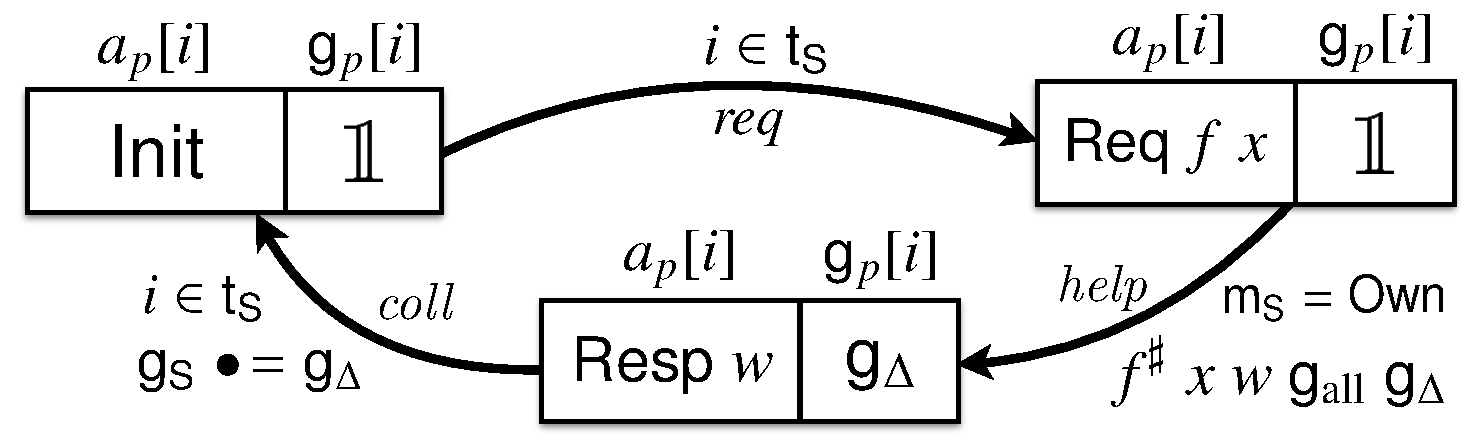
\includegraphics[width=0.60\textwidth]{fctrans.pdf}    
\end{center}
%
%\vspace{5pt}
%
The transition $\reqtrans$ can be taken only by a thread holding the
thread id $i$; it changes the value of $\ap[i]$ from $\Done$ to
$\Req{f}{x}$ for some $f$ and $x$.
%
The transition $\helptrans$ can be performed by any thread that owns
the lock (not necessarily the one with the id $i$); it replaces the
contents of $\ap[i]$ and $\gp[i]$ with an appropriate result $w$ and
an auxiliary delta $\gd$, respectively. The two are valid \wrt~the
input $x$ and the cumulative auxiliary $\gall$, as ensured by the
constraint $\fspec{f}$.
%
Finally, $\colltrans$ is invoked by the thread with id $i$; it flushes
the contents of $\gp[i]$, into the self-contribution $\gs$ and puts
$\Done$ into $\ap[i]$.

\subsection{Flat combiner specification}
\label{sec:fc-conc-spec}


We now provide a spec for \code{flatCombine} in terms of the
concurroid $\fccon$. We assume $f : A \to B$, $x : A$, and $f$ comes
with the following spec.\footnote{Thus, we don't require $f$ to be
  sequential (\ie, in addition to just manipulating the
  privately-owned state, $f$ can also allocate new concurroids via
  hiding, and fork children threads), but every sequential function
  can be given a spec in~$\privcon$.}
%
\[
\tag{\normalsize \arabic{tags}}\refstepcounter{tags}\label{eq:fspec}
{\small
\hspace{-5pt}
\begin{array}{c}
\sspec{~
\exists h\ldot \hpriv \spts h \aand I~\g~h
~} 
~~f(x)~~
\sspec{~
\exists h'~\gd\ldot\hpriv \spts h' \aand I~(\g \join \gd)~h' \aand
\fspec{f}~x~\res~\g~\gd
~}@\privcon
\end{array}
}\]
%
The spec allows the input heap $h$ to change to $h'$. The resource
invariant $I$ has to be preserved, up to a change of the auxiliary
state, from $\g$ to $\g \join \gd$. $\fspec{f}$ is a client-supplied
predicate which specifies $f$. We call it \emph{validity predicate};
it's functional with respect to~$\gd$, and relates the input value
$v$, the result value~$\res$, the initial auxiliary state~$\g$ and the
``auxiliary delta'' $\gd$ resulting from the invocation of~$f$.
%
For instance, if $f$ were a sequential push operation on stacks, with
$\g$ and $\gd$ being set to histories $\hist$ and $\histd$, we might
choose the following validity predicate:
%
\[
\tag{\normalsize \arabic{tags}}\refstepcounter{tags}\label{eq:push-spec}
{\small
%\hspace{-4.1mm}
\begin{array}{r@{\ }c@{\ }l}
  \fspec{\push}~x~\res~\hist~\histd & \eqdef & \res = () \aand \histd =
  \tfr{\hist} \hpts (l, x::l),
\end{array}
}\] 
%
where $l = \hist[\last{\hist}]$. That is, $\fspec{\push}$ fixes the
result of $\push$ to be unit and its effect to be the singleton
history describing the action of pushing.

%
%We require that $f$ preserves the invariant $I$. 
%The  operates over the private heaps only, it can be
%considered as sequential. 
%spec~\eqref{eq:fspec} is indeed sequential, as it captures only
%elements of the privately-owned heap and can possibly make use of the
%unconstrained allocator.

For the \code{flatCombine} spec, we need two auxiliary predicates.
$\NoReqs$ indicates that the thread $\tid$ doesn't request
help. $\histso{\cdot}{\cdot}$, generalizes~\eqref{eq:histso} from
histories to PCM~$\pcmS$.
%
\[
\tag{\normalsize \arabic{tags}}\refstepcounter{tags}\label{eq:noreqs}
{\small
\begin{array}{rcl}
\noreqs{\tid} & \eqdef & \hfc \spts (\set{\tid}, \lockNown, -) \aand
\ap[\tid] = \Done     
\\[5pt]
\histso{\hfc}{\gS, \gO, \g} & \eqdef &\hfc \spts  (-, -, \gS)
  \aand 
\hfc \opts (-, -, \gO) \aand
\g \pre \jjoin{i}\gp[i] \join \gS \join \gO    
\end{array} 
}
\] 
%
%\hspace{-5pt}
%
Here, the partial order $\pre$ on PCM elements is defined as $\g_1
\pre \g_2 \eqdef \exists \g, \g_2 = \g_1 \join \g$. It generalizes the
relation $\pre$ from histories to the PCM $\pcmS$, and in the
specs captures that the value $\g_1$ was ``current'' before $\g_2$.
%

The spec for \code{flatCombine} is given \wrt a specific thread id
$\tid$.
%
%\vspace{-5pt}
%
\[
\tag{\normalsize \arabic{tags}}\refstepcounter{tags}\label{eq:fc-spec}
{\small
\hspace{-10pt}
\begin{array}{c}
\spec{
  \hpriv \spts \hempty ~\sep~ \histso{\hfc}{\pcmU, -, \g} \aand
  \noreqs{\tid} 
} 
\\
\eesc{flatCombine}(f, x): B
\\
\spec{
\begin{array}{c}
\exists \g'~\gd\ldot \hpriv \spts \hempty ~\sep~
\histso{\hfc}{\gd, -, \g'} \aand \noreqs{\tid} \aand 
\g \pre \g' \aand
\fspec{f}~x~\res~\g'~\gd 
\end{array}
}@\privcon\entangle\fccon
\end{array}
}
\]
%
%
A call to \code{flatCombine} starts and ends in a state in which the
thread $\tid$ doesn't request the help ($\NoReqs$), and in which $\g$
names the sum total of the contributions. It doesn't change the
privately-owned heap, but increases self-contribution by amount of an
auxiliary delta $\gd$. The mediating value $\g'$ is a sum-total of the
contributions at the moment when the thread received help; thus,
$\fspec{f}~x~\res~\g'~\gd$. As $\g'$ is current sometime after the
initial $\g$, the spec postulates $\g \pre \g'$.
%
%relating the input and result values with $\gd$ using $\fspec{f}$:
%$\g'$ captures the overall auxiliaries combined at \emph{some moment}
%during the execution of \code{flatCombine}. Using $\g$ for this
%purpose would make the postcondition non-stable.
%
Due to space limitations, we omit a detailed discussion on
verification of the spec~\eqref{eq:fc-spec} of the flat combiner (it
can be found in Appendix~\ref{sec:verifying-fc} or in the accompanying
Coq files).

To strengthen the analogy with coarse-grained CSL-style locks, let us
note that if one were to implement a procedure
$\eesc{coarseGrainedCombine}(f, x)=\eesc{\{}
\eesc{lock}();~f(x);~\eesc{unlock}() \eesc{\}}$, its specification
would be the same as~\eqref{eq:fc-spec}, modulo the $\NoReqs$ conjunct
and the join with all $\gp[i]$ components in \eqref{eq:noreqs}, which
would not be present in the coarse-grained case, as they are artefacts
of the helping machinery.\footnote{To provide truly \emph{the same}
  specs, one would need to introduce abstract predicates to hide these
  artefacts, but we can do that in Coq, so we omitted the discussion
  on them in this paper.}

\subsection{Instantiating the flat combiner for stacks}
\label{sec:instantiating-fc}

To illustrate that the abstract spec for the flat combiner follows the
expected intuition, we consider an instance where $\gS, \gO, \gp$ are
histories, and $f$ is the sequential \code{push} method for stacks,
satisfying~the generic sequential spec~\eqref{eq:fspec} with the
validity predicate $\fspec{\push}$ defined by~\eqref{eq:push-spec} and
the stack invariant~\eqref{eq:tb-states}.
%
%A sequential implementation of $\push$ would come with the following
%accompanying validity predicate $\fspec{\push}$:
%
%
%\[
%\tag{\normalsize \arabic{tags}}\refstepcounter{tags}\label{eq:push-spec}
%{\scriptsize
%%\hspace{-4.1mm}
%\begin{array}{r@{\ }c@{\ }l}
%  \fspec{\push}~x~w~\hist~\histd & \eqdef & w = () \aand \histd =
%  \tfr{\hist} \hpts (l, x::l),
%\end{array}
%}\]
%%
%where $l = \hist[\last{\hist}]$. That is, $\fspec{\push}$ fixes the
%result of $\push$ to be unit and its effect to be the singleton
%history describing the ``push''. 
%
So by instantiating~\eqref{eq:fc-spec}, after some simplification, we
obtain:
%
\[
\tag{\normalsize \arabic{tags}}\refstepcounter{tags}\label{eq:fc-push-spec}
{\small
\begin{array}{c} 
\spec{
\begin{array}{c} 
  \hpriv \spts \hempty ~\sep~
  \histso{\hfc}{\hempty, -, \hist} \aand
  \noreqs{\tid} 
\end{array}
} 
\\
\eesc{flatCombine}(\push, e): \mathsf{Unit}
\\
\spec{
\begin{array}{c}
\exists t~l\ldot \hpriv \spts \hempty ~\sep~
\histso{\hfc}{t \hpts (l, e::l), -, \hist} \aand
\hist < t \aand
\noreqs{\tid}
\end{array}
}
%@(\privcon\acon)\entangle\fccon
\end{array}
}
\]
%
Note that~\eqref{eq:fc-push-spec} is very similar to the spec
\eqref{eq:stack-spec} for Treiber \code{push}; the only difference,
again, is in the FC-specific components such as thread id's, the
$\NoReqs$ predicate, and the lock status views used in the definition
of $\NoReqs$. Thus, the spec~\eqref{eq:fc-spec} is adequate.
%
A similar derivation can be done for an FC-specification of $\pop$.



\section{Related Work}
\label{sec:related}

% Existing methods for specifying the behavior of concurrent data
% structures and programs are either history-based or state-based.
% %
% The former ones describe the behavior of an object by describing and
% characterizing call/return strings that can be obtained by invoking
% the methods concurrently by several threads. 
% %
% The later ones define the object's behavior by posing requirements to
% a state, in which object's methods are safe to run, and stating
% assertions over a state, resulting from the object's method call. The
% second group of approaches employs program logics as a way to specify
% the state of interest as well as a mechanism to compose the program
% specifications.

% This paper contributes to the goal of unifying the history- and
% state-based views to specification and verification of concurrent
% objects.

% In this section we describe related approaches for reasoning about
% concurrency that have motivated our work.

\paragraph{Linearizability and history-based criteria.}

% In the past 25 years, linearizability has been widely applied to
% capture the behavior of concurrent objects with intuitive sequential
% specifications, and even suitable for automatic synthesis of some
% concurrent objects~\cite{Vechev-Yahav:PLDI08}. Thanks to the
% compositional proof method, based on \emph{linearization points},
% proofs of linearizability in most of the cases are amenable for
% practical computer-aided
% verification~\cite{Burckhardt-al:PLDI10,Derrick-al:TOPLAS11,Vafeiadis:CAV10,Amit-al:CAV07,Shacham-al:OOPSLA11,Dragoi-al:CAV13}.

The need for correctness criteria alternative to
linearizability~\cite{Herlihy-Wing:TOPLAS90}, which is more relaxed
yet compositional, was recognized in the work on counting
networks~\cite{Aspnes-al:JACM94}.
%
The suggested notion of quiescent
consistency~\cite{Shavit-Zemah:TOPLAS96} required the operations
separated by a quiescent state to take effect in their logical order.
%
%
A more refined correctness condition, \emph{quasi-linearizability},
implementing a relaxed version of linearizability with an upper bound
on nondeterminism, was proposed by Afek~\etal~\cite{Afek-al:OPODIS10},
allowing them to obtain the quantitative boundaries similar to what we
proved in Section~\ref{sec:qqc-client}.
%
The idea of relaxed linearizability was later used in the work on
\emph{quantitative relaxation} (QR)~\cite{Henzinger-al:POPL13} for
designing scalable concurrent data structures by changing the
specification set of sequential histories.
%
Most recently, \emph{quantitative quiescent consistency} has been
proposed as another criterion incorporating the possibility to reason
about effects of bounded thread
interference~\cite{Jagadeesan-Riely:ICALP14}.
%
It is worth noticing that some of these correctness criteria are
incomparable (\eg, QC and QR~\cite{Henzinger-al:POPL13}, QL and
QQC~\cite{Jagadeesan-Riely:ICALP14}) hence, for a particular
concurrent object, choosing one or another criterion should be
justified by the needs of the object's client. Therefore, a suitable
correctness condition is essentially ``\emph{in the eye of the
  beholder}'', as is typical in programming, when designing libraries
and abstract data structures, and the logic-based approach we advocate
provides precisely this flexibility in choosing desired specs.

% However, how suitable is one or another relaxed correctness
% condition %from the listed ones
% for reasoning about safety properties of a particular client program
% is still largely an open question.

\paragraph{Hoare-style specifications of concurrent objects.}
\label{sec:related-logic-based}

% Program logics for concurrency allow one to capture in the
% specification precisely those bits of information about the program's
% state, which are relevant for the program's clients, making it
% possible to abstract over the irrelevant details of the
% implementation~\cite{DinsdaleYoung-al:ECOOP10}.

Hoare-style program logics were used with great success to verify a
number of concurrent data structures and algorithms, which are much
more natural to specify in terms of observable state modifications,
rather than via call/return histories. The examples of such objects
and programs include
barriers~\cite{Dodds-al:POPL11,Hobor-Gherghina:ESOP11}, concurrent
indices~\cite{ArrozPincho-al:OOPSLA11}, flat
combiner~\cite{Turon-al:ICFP13,Sergey-al:ESOP15}, event
handlers~\cite{Svendsen-Birkedal:ESOP14}, shared graph
manipulations~\cite{Raad-al:ESOP15,Sergey-al:PLDI15}, as well as their
multiple client programs.
%
The observation about a possibility of using program logics as a
correctness criterion, alternative to linearizability, has been made
in some of the prior
works~\cite{Jacobs-Piessens:POPL11,ArrozPincho-al:OOPSLA11,Svendsen-al:ESOP13}.
%
Their criticism of linearizability addressed its inability to capture
the state-based properties, such as dynamic memory
ownership~\cite{Jacobs-Piessens:POPL11}---something that
linearizability indeed cannot tackle, unless it's
extended~\cite{Gotsman-Yang:CONCUR12}.
%
However, we are not aware of any prior attempts to capture CAL, QC and
QQC-like properties of concurrent executions by means of \emph{one and
  the same} program logic and employ them in client-side
reasoning.

%
% Verification in such logics is done structurally, \ie, by
% systematically applying syntax-directed inference rules, until the
% spec is proved. Several mechanized tools for logic-based
% concurrent reasoning have been
% released~\cite{Sergey-al:PLDI15,Appel-al:BOOK14}.

Several logics for proving linearizability or, equivalently,
observational refinement~\cite{Filipovic-al:TCS10,Turon-al:POPL13},
have been proposed
recently~\cite{Turon-al:ICFP13,Liang-Feng:PLDI13,Vafeiadis:PhD}, all
employing variations of the idea of using \emph{specifications as
  resources}, and identifying (possibly, non-fixed or non-local)
linearization points, at which such specification should be ``run''.
%
In these logics, after establishing linearizability of an operation,
one must still devise its Hoare-style spec, such that the spec is useful for
the clients.
% %
% To avoid this detour, a number of other logic-based approaches have
% suggested to assign Hoare-style specifications \emph{directly} to
% fine-grained object
% implementations~\cite{Svendsen-al:ESOP13,Svendsen-Birkedal:ESOP14,ArrozPincho-al:ECOOP14}
% and reason out of these specs.

Similarly to the way linearizability allows one to replace a
concurrent operation by an atomic one, several logics have implemented
the notion of \emph{logical atomicity}, allowing the clients of a data
structure to implement application-specific synchronization on top of
the data structure operations.
%
Logical atomicity can be implemented either by parametrizing specs
with client-specific auxiliary
code~\cite{Jacobs-Piessens:POPL11,Svendsen-al:ESOP13,Svendsen-Birkedal:ESOP14,Jung-al:POPL15}
or by engineering dedicated rules relying on the simulation between
the actual implementation and the ``atomic''
one~\cite{ArrozPincho-al:ECOOP14}.
%
% Both approaches to logical atomicity require one to identify precisely
% a \emph{synchronization point}~\cite{Svendsen-al:ESOP13} within the
% structure being verified, which makes it non-trivial to apply them for
% specifying non-linearizable objects, especially when conducting
% quantitative logic-based reasoning, which we demonstrated in
% Section~\ref{sec:qqc-client}.

Instead of trying to extend the existing approaches for logical
atomicity to non-linearizable objects (for which the notion of
atomicity is not intuitive), we relied on a general mechanism of
auxiliary state, provided by FCSL~\cite{Nanevski-al:ESOP14}. 
%
Specifically, we adopted the idea of histories as auxiliary
state~\cite{Sergey-al:ESOP15}, which, however, was previously explored
in the context of FCSL only for specifying linearizable structures.
%
% Similarly to logical atomicity, the histories-as-state specification
% approach makes fine-grained concurrent programs look like atomic ones,
% since due to compositionality, the specification clients only see the
% history entries.
%
% 
We introduced enhanced notation for referring directly to histories
(\eg, $\hists$, $\histo$), although FCSL's initial logical
infrastructure and inference rules remained unchanged.

% Recently, attempts were made to unify the common idioms occurring in a
% number of concurrency logics in a generic framework of
% \emph{Views}~\cite{DinsdaleYoung-al:POPL13}.
% %
% However, that result is orthogonal to our findings, as \emph{Views}
% are a framework for proving logics sound, not to prove programs, and
% this paper, we focused on using a particular logic (FCSL) for specifying a
% new class of concurrent data structures.
The purpose of \emph{Views}~\cite{DinsdaleYoung-al:POPL13} is to provide a PCM-based semantic framework for proving soundness of logics and type systems, and thus to unify common idioms occurring in several recent concurrency logics. However, the framework has not used PCMs for auxiliary state and/or specification of user programs. \ab{Please check.}


In this work, we do not argue that FCSL is the only logic capable of
encoding custom correctness conditions and their combinations, though,
we are not aware of any other work exploring a similar possibility.
%
However, we believe that FCSL's explicit \emph{other}
subjective state component provides the most straightforward way to do
so.
%
The logics like CAP~\cite{DinsdaleYoung-al:ECOOP10} and
TaDA~\cite{ArrozPincho-al:ECOOP14}, from our experience and personal
communication with their authors, may be capable of implementing our
approach at the expense of engineering a much more complicated
structure of capabilities to encode histories and their invariants,
and ``snapshot'' interference of an environment.
%
Other logics incorporating the generic PCM
structure~\cite{Raad-al:ESOP15,Jung-al:POPL15,Jung-al:ICFP16,Turon-al:OOPSLA14}
might be able to implement our approach, although none of these logics
provide an FCSL-style rule for hiding~\eqref{eq:ehide} as a uniform
mechanism to express explicit quiescence.

%\todo{State that in our cases histories are per-object.}

Concurrently with this work, Hemed~\etal developed a (not yet
mechanized) verification technique for CAL~\cite{Hemed-al:DISC15},
which they applied to the exchanger and the elimination
stack. Similarly to our proposal, they specify CAL-objects via Hoare
logic, but using one global auxiliary history, rather than subjective
auxiliary state. 
%
This tailors their system specifically to CAL (without a possibility
to incorporate reasoning about other, non CA-linearizable, concurrent
structures), and to programs with a \emph{fixed} number of threads. In
contrast, FCSL supports dynamic thread creation, and is capable of
uniformly expressing and mechanically verifying several different
criteria, with CAL merely a special case, obtained by a special choice
of PCM. Moreover, in FCSL the criteria combine, as illustrated in
Section~\ref{sec:cal}, where we combined quiescence with CAL via
hiding. Hiding is crucial for verifying clients with explicit
concurrency, but is currently unsupported by Hemed~\etal's method.
%
% Related is the property of our histories that no event may appear
% between two twin timestamps. We used this property to verify the
% client in Section~\ref{sec:cal}, but this does not seem to hold for
% histories used by Hemed~\etal

%Concurrently with our work, Hemed~\etal developed a (not yet
%mechanized) verification technique for
%CAL~\cite{Hemed-al:DISC15}. Similarly to our proposal, they employed
%the idea of specifying CAL-objects via Hoare triples with auxiliary
%histories. Unlike our approach, their choice of abstractions is
%tailored for conducting proofs about CAL, and they don't establish a
%soundness result of their Hoare-style specs, with respect to CAL or
%any other semantics. In contrast, what we propose is using a uniform
%framework, proved sound from first principles~\cite{Sergey-al:PLDI15},
%capable of capturing the essence of multiple correctness conditions
%(including CAL) and verifying them mechanically. Our spec of the
%exchanger~\eqref{tag:exchangespec} can be easily generalized to tackle
%verification of the elimination stack (main example
%from~\cite{Hemed-al:DISC15}) by parametrizing it with a
%client-provided invariant on histories. Furthermore, by using FCSL as
%a logical foundation, we can also reason about quiescence (via hiding)
%and dynamic thread spawning (via the rule~\eqref{eq:parrule}). These
%components are crucial for verifying clients featuring explicit
%concurrency (Section~\ref{sec:cal}), and we currently don't see how to
%conduct such proofs out of the spec from~\cite{Hemed-al:DISC15}.


% \paragraph{Reasoning about linearizability in program logics}
% \label{sec:rel-linear}

% \begin{itemize}

% \item Logics for linearizability (viktor's PhD), LF, Turon, contextual refinement

% \item Hindsight paper by O'Hearn and company

% \item Observation from the HOCAP paper about the push2 method, that,
%   however, never were extended to any interesting structures, so we
%   did it.

% \item Abstract atomicity

% \end{itemize}


%\vspace{-4pt}

\section{Conclusion and Future Work}
\label{sec:conclusion}

%\vspace{-2pt}

In this paper we have presented a number of formalization techniques,
enabling specification and verification of highly scalable
non-linearizable concurrent objects and their clients in Hoare-style
program logics.
%
Specifically, we have explored several reasoning patterns, all
involving the idea of formulating execution histories as an instance
of auxiliary state and then making these histories to be a subject of
object-specific invariants, capturing the expected concurrent object
behavior.
%
In particular, we have discovered that quantitative logic-based
reasoning about concurrent behaviors can be done by storing relevant
information about interference directly into the entries of a logical
auxiliary history, a pattern which we later demonstrated to be
beneficial in the client-side proofs.

We believe that our results help to bring the Hoare-style reasoning
approach into the area of non-linearizable concurrent data structures
and open a number of exciting opportunities for the field of
logic-based concurrency verification.

For instance, by ascribing interference-sensitive quantitative specs
in the spirit of~\eqref{eq:qc-spec} to relaxed concurrent
libraries~\cite{Henzinger-al:POPL13}, one can assess the applicability
of a particular library implementation for its clients, that can
tolerate the anomalies caused by interference, as long as they can
logically infer the desired safety assertions from the library spec,
as we did in Section~\ref{sec:qclients}.
%
Since logical approaches enable reasoning about higher-order
concurrent data
structures~\cite{Svendsen-al:ESOP13,Turon-al:ICFP13,Sergey-al:ESOP15},
we envision the possibility of giving parametric logical specs to such
generic relaxed constructions as diffracting/elimination
trees~\cite{Shavit-Touitou:TCS97,Shavit:CACM11} that, once
instantiated with suitably specified stacks or pools on the leaves,
would yield a provably correct, highly scalable concurrent container
implementation.


% Acknowledgements:

% Michael Emmi
% Pierre Ganty
% Andrea Cerone
% Anton Podkopaev

% \todo{Generalizing the construction of the counting network to
%   arbitrary diffracting trees}

% \todo{Elimination and diffracting trees~\cite{Shavit-Touitou:TCS97}.}

 
%\setlength{\bibsep}{2.2pt}

\bibliographystyle{abbrv}
\bibliography{bibmacros,references,proceedings-short}

% \newpage
% \appendix
% %\softraggedright 

\setlength{\parindent}{0.0in}
\setlength{\parskip}{5pt}
\titlespacing*{\section}{0pt}{*1}{*1}
\titlespacing*{\subsection}{0pt}{*0.7}{*0.5}
\titlespacing*{\paragraph}{0pt}{*0.5}{*0.5}


\section*{Optional appendices}

In the optional appendices we provide detailed overview of main
concepts of Fine-grained Concurrent Separation Logic~(FCSL), necessary
for the formal reasoning. These include semantics of the logical
assertions as well as inference rules. We address the curious reader
to the original paper on FCSL~\cite{Nanevski-al:ESOP14} and its
extended version (or the Coq development accompanying this manuscript)
for the details of FCSL's denotational semantics and the soundness
proof.
%
\textbf{Appendix~\ref{sec:broccoli}} provides the formal semantics of
the FCSL assertions.
%
\textbf{Appendix~\ref{app:conc}} formally presents concurroids and
entanglement, along with several examples.
%
\textbf{Appendix~\ref{sec:appactions}} describes properties of
atomic actions of FCSL concurroids.
%
\textbf{Appendix~\ref{sec:rules}} provides the rules of FCSL,
explaining some of them in detail.
%
Finally, \textbf{Appendix~\ref{sec:verifying-fc}} describes in detail
the veritifaction of the flat combiner specification~\eqref{eq:fc-spec}
from Section~\ref{sec:flatco} and presents the proof outline.

\section{Semantics of FCSL assertions}
\label{sec:broccoli}

State in FCSL is divided along two different axes. The first axis is
labels (isomorphic to $\mathsf{nat}$). Labels identify concurroids,
\ie data structures that are stored in the state, with specific
restrictions on their evolution. The second axis is ownership. Each
label contains self, other and joint component, describing how much of
each concurroid is owned privately by the specified thread, privately
by that thread's environment, and how much is shared, respectively.

To formally define the concept, we introduce the notion of PCM-map and
type-maps.  A PCM-map is a finite map from labels to a dependent
product $\Sigma_{{\pcmS}{:}\textrm{pcm}} \pcmS$, where
$\mathbb{U}$ is a PCM, and $v \in \pcmS$. A type map is similar,
except we don't require the range to be a PCM; it can be an arbitrary
type.

PCM-maps are composed by means of two operations. Disjoint union $m_1
\hunion m_2$ collects the labels from $m_1$ and $m_2$, ensuring that
there's no overlap. This operation applies to type-maps as well.
%
However, PCM-maps have another operation which doesn't apply to
type-maps: $m_1 \zip m_2$ joins the values of individual labels, \ie,
$\hempty \zip \hempty = \hempty$, and $((\hlabel \hpts_{\pcmS}
v_1) \hunion m'_1) \zip ((\hlabel \hpts_{\pcmS} v_2) \hunion m'_2)
= (\hlabel \hpts_{\pcmS} v_1 \join v_2) \hunion (m'_1 \zip m'_2)$,
and undefined otherwise.

State, ranged over by $w$, is a triple $\state{s}{j}{o}$, where~$s$
and~~$o$ are PCM-maps, and $j$ is a type map. We refer to them as
\emph{self}, \emph{other}, and \emph{joint} components of $w$.  In
specifications, the three components signify different state
ownership: $s$ is the state owned by the specified thread, and is
inaccessible to the environment; $o$ is the state owned by the
environment, and is inaccessible to the specified thread; $j$ is the
shared (or joint) state, accessible to every thread.
%
Notice that unlike $s$ and $o$ which are PCM-maps, $j$ is a
type-map. In other words, the joint component is not subject to
PCM-laws, as we don't shuffle its components upon forking, joining,
and framing, as we do in the cases of $s$ and $o$.

The state $w = \state{s}{j}{o}$ is valid iff:
\begin{itemize}
\item[$(i)$] the components $s$, $j$ and $o$ contain the same labels.
 
\item[$(ii)$] $s\ {\zip}\ o$ is defined, \ie, equals labels in $s$ and $o$
  contain equal PCMs. Notice that the labels in $j$ are independent,
  and may contain elements of other types;
\item[$(iii)$] the heaps that may be stored in the labels of $s$, $j$,
  $o$ are disjoint.
\end{itemize}

Figure~\ref{fig:broccoli} collects the definitions the main assertions
of FCSL in terms of the two operations on PCM-maps.
%

\begin{figure}[t]
\[
{\small
\begin{array}[t]{l@{\,}l}
  w \models \top & \mbox{iff always}\\
  w \models \hlabel \spts v & \mbox{iff valid $w$, and $w = w_1 \hunion
    w_2$, and $w_1.\mathself = \hlabel \hpts v$}\\ 
  w \models \hlabel \jpts h & \mbox{iff valid $w$, and $w = w_1 \hunion
    w_2$, and $w_1.\mathjoint = \hlabel \hpts v$}\\ 
  w \models \hlabel \opts v & \mbox{iff valid $w$, and $w = w_1 \hunion
    w_2$, and $w_1.\mathother = \hlabel \hpts v$}\\ 
  w \models p \aand q & \mbox{iff $w \models p$ and $w \models q$}\\
  w \models p \lsep q & \mbox{iff valid $w$, and $w = w_1 \hunion w_2$, and $w_1 \models p$ and $w_2 \models q$}\\
  w \models p \wand q & \mbox{iff for every $w_1$, valid $w \hunion w_1$, $w_1 \models p$ implies $w \hunion w_1 \models q$}\\
  w \models p \ssep q & \mbox{iff valid $w$, and $w.\mathself= \mathself_1 \hunion \mathself_2$, and}\\
  & \hphantom{\mbox{iff}}\ \mbox{$\state{\mathself_1}{w.\mathjoint}{{\mathself_2} \zip {w.\mathother}}
    \models p$ and $\state{\mathself_2}{w.\mathjoint}{{\mathself_1} \zip
      {w.\mathother}} \models q$}\\
  w \models \mathsf{this}\ w' & \mbox{if $w = w'$}\\
  \hphantom{w} \models p \downarrow h & \mbox{iff for every valid $w$, $w
    \models p$ implies $\flatten w = h$}
  \\
  \\
  \mbox{valid $w$} & \mbox{iff $w=\state{\mathself}{\mathjoint}{\mathother}$, 
                           $\mathsf{dom}\,\mathself = \mathsf{dom}\,\mathjoint = \mathsf{dom}\,\mathother$,}\\
  & \mbox{ $\mathself\,{\zip}\,\mathother$ is defined, 
           and the heaps in $\mathself$, $\mathjoint$, $\mathother$
           are disjoint}
         \\\\
  \flatten w & \eqdef \mbox{ disjoint union of all the heaps in $w$}
  \\\\
  w_1 \hunion w_2 & \eqdef \mbox{pairwise disjoint union of $w_{1,2}$'s
    PCM-components}
  \\\\
  \hlabel \hpts \state{{v_s}}{{v_j}}{{v_o}} & \eqdef \mbox{ $\state{{\hlabel \hpts v_s}}{{\hlabel \hpts v_j}}{{\hlabel \hpts v_o}}$}
\end{array}}
\]
\caption{Notation and semantics of main FCSL assertions.}
\label{fig:broccoli}
\end{figure}
%

\section{Concurroids: properties and examples}
\label{app:conc}

A concurroid is a 4-tuple $\ucon = (L, W, I, {E})$ where:
(1) $L$ is a set of labels, where a label is a nat; (2) $W$
is the \emph{set of states}, each state $w \in W$ having the
structure described in Section~\ref{sec:broccoli}; (3) $I$ is the
set of \emph{internal transition}, which are relations on $W$
and one of which is always an identity
relation $\id$; (4) $ E$ is a 
set of pairs $(\alpha, \rho)$, where $\alpha$ and $\rho$ are
\emph{external transitions} of $\ucon$. An external transition is a
function, mapping a heap $h$ into a relation on $W$. The
components must satisfy a further set of requirements, discussed next.

%\vspace{5pt}

\paragraph{State properties.}

Every state $w \in W$ is $\mathsf{valid}$ as defined in
Figure~\ref{fig:broccoli}, and its label footprint is $L$, \ie
$\mathsf{dom}\ (w.\mathself) = \mathsf{dom}\ (w.\mathjoint) =
\mathsf{dom}\ (w.\mathother) = {L}$. Additionally, $W$
satisfies the property:
%
\begin{mathpar}
{\small
\begin{array}{ll}
\textit{Fork-join closure:} & \forall t{:}\textrm{PCM-map}\ldot w \zig t \in {W} \iff w \zag t \in {W}, \\
& \mbox{where}\ w \zig t = \state{t \zip
  w.\mathself}{w.\mathjoint}{w.\mathother}, 
\\
&\mbox{and}\ w \zag t = \state{w.\mathself}{w.\mathjoint}{t \zip w.\mathother}
\end{array}
}
\end{mathpar}
% 
The property requires that $W$ is closed under the realignment of
\self and \other components, when they exchange a PCM-map $t$ between
them. Such realignment is part of the definition of $\ssep$, and thus
appears in proofs whenever the rule \textsc{Par}~\eqref{eq:parcom} is
used, \ie whenever threads fork or join. Fork-join closure ensures
that if a parent thread forks in a state from $W$, then the child
threads are supplied with states which also are in $W$, and
dually for joining.

%\vspace{5pt}

\paragraph{Transition properties.}

A concurroid transition $\gamma$ is a relation on $W$ satisfying:
%
\begin{mathpar}
{\small
\begin{array}{ll}
\textit{Guarantee:} & (w, w') \in \gamma \implies w.\mathother =
w'.\mathother
\\[5pt]
\textit{Locality:} & \forall t{:}\textrm{PCM-map}\ldot 
  w.\mathother = w'.\mathother \implies\\
&  (w \zag t, w' \zag t) \in \gamma \implies (w \zig t, w' \zig t) \in \gamma
\end{array}
}
\end{mathpar}
%
Guarantee restricts $\gamma$ to only modify the \self and \joint
components. Therefore, $\gamma$ describes the behavior of a viewing
thread in the subjective setting, but not of the thread's
environment. In the terminology of Rely-Guarantee
logics~\cite{Feng-al:ESOP07,Feng:POPL09,Vafeiadis-Parkinson:CONCUR07},
$\gamma$ is a \emph{guarantee} relation. To describe the behavior of
the thread's environment, \ie, obtain a \emph{rely} relation, we
merely \emph{transpose} the self and other components of~$\gamma$.
%
\[
\tag{\arabic{tags}}\refstepcounter{tags}\label{eq:transp}
{\small
\gamma^\top = \{(w_1^\top, w_2^\top) \mid (w_1, w_2) \in \gamma\},\ 
\mbox{where $w^\top = \state{w.\mathother}{w.\mathjoint}{w.\mathself}$}
}
\]
% 
In this sense, FCSL transitions always encode \emph{both} guarantee
and rely relations.

Locality ensures that if $\gamma$ relates states with a certain \self
components, then $\gamma$ also relates states in which the \self
components have been simultaneously \emph{framed} by a PCM-map $t$,
\ie, enlarged according to $t$. It thus generalizes the notion of
locality from separation logic, with a notable difference. In
separation logic, the frame $t$ materializes out of nowhere, whereas
in FCSL, $t$ has to be appropriated from \other; that is, taken out
from the ownership of the environment.

An \emph{internal} transition $\iota$ is a transition which preserves
heap footprints. An \emph{acquire} transition $\alpha$, and a
\emph{release} transition $\rho$ are functions mapping heaps to
transitions which extend and reduce heap footprints, respectively, as
show below.  An external transition is either an acquire or a release
transition. If $(\alpha, \rho) \in  E$, then $\alpha$ is an
acquire transition, and $\rho$ is a release transition.
%
\begin{mathpar}
{\small
\begin{array}{lcl}
\textit{Footprint preservation} & : & 
 (w, w') \in \iota \implies \mathsf{dom}\ \flatten{w} = \mathsf{dom}\
 \flatten{w'}
\\[5pt]
\textit{Footprint extension} & : &
 \forall h{:}\mathrm{heap}\ldot (w, w') \in \alpha(h) \implies
\\ 
&& \mathsf{dom}\ (\flatten{w} \hunion h) = \mathsf{dom}\ \flatten{w'}
\\[5pt]
\textit{Footprint reduction} & : &
 \forall h{:}\mathrm{heap}\ldot (w, w') \in \rho(h) \implies
 \\
 &&\mathsf{dom}\ (\flatten{w'} \hunion h) = \mathsf{dom}\ \flatten{w}
\end{array}
}
\end{mathpar}
%
The set of Internal transitions always includes at least the identity
transition $\id$ (\ie, transition from a state to itself). Footprint
preservation requires internal transitions to preserve the domains of
heaps obtained by state flattening. Internal transitions may exchange
the ownership of subheaps between the \self and \joint components, or
change the contents of individual heap pointers, or change the values
of non-heap (\ie, auxiliary) state, which flattening erases. However,
they cannot add new pointers to a state or remove old ones, which is
the task of external transitions, as formalized by Footprint extension
and reduction.

\subsection{The concurroid of private heaps}
\label{sec:conc-priv-heaps}

The private heap concurroid is defined as follows.
%
\[
\tag{\arabic{tags}}\refstepcounter{tags}\label{eq:privcon}
\privcon = (\{\hpriv\}, {W}_{\privcon}, \set{\iota_{\privcon},
  \id}, \{(\alpha_{\privcon}, \rho_{\privcon})\})
\]
%
It is identified by a \emph{fixed} dedicated label $\hpriv$
%
and directly captures the notion of heap \emph{ownership}, as presented in
CSL~\cite{OHearn:TCS07}.
%
Its state-space ${W}_{\privcon}$ is defined as a set of states of the
shape
%
\[
\hpriv \hpts \state{\hL}{\hempty}{\hE},
\]
%
where $\hS$ and $\hO$ are disjoint heaps (which are known to form a
PCM). The concurroid's \emph{internal} transitions $\iota_{\privcon}$
allow the values in the codomain of the heap $\hL$, privately-owned by
\emph{self}, to be changed arbitrarily. There is only one channel of
acquire/release transitions $\alpha_{\privcon}$ and $\rho_{\privcon}$
that account for the addition/removal of a heap chunk to/from~$\hL$
correspondingly, given that the state validity is
preserved. Transitions of~$\privcon$ can be formally defined using the
notation from Figure~\ref{fig:broccoli} as follows:
%
\[ 
\tag{\arabic{tags}}\refstepcounter{tags}\label{eq:priv-trans}
{\small
  \begin{array}{lcr@{\ \ }c@{\ \ }l}
    \iota_\privcon & \eqdef & \hpriv \spts (x \hpts v \hunion \hL) & {\rightsquigarrow} &
    \hpriv \spts {(x \hpts w \hunion \hL)}
    \\
    \alpha_\privcon(h) & \eqdef & \hpriv \spts \hL & {\rightsquigarrow} &
    \hpriv \spts {(\hL \hunion h)}
    \\
    \rho_\privcon(h) & \eqdef & \hpriv \spts (\hL \hunion h) & {\rightsquigarrow} & \hpriv \spts {\hL}
  \end{array}
}\]
%
Importantly, as demonstrated by the rule fo
hiding~\eqref{eq:hide-rule}, the concurroid $\privcon$ serves as the
primary one in FCSL: all other concurroids are it in a scoped manner
via the \emph{hiding} mechanism (see Appendix~\ref{sec:rules}).
%
In order to describe allocation/deallocation, the private heap
concurroid is typically being entangled with an allocator concurroid
$\acon$, which we have implemented in Coq as an instance of a
spin-lock with a specific resource invariant (see
Section~\ref{sec:concurroid-spin-lock}), but omitted from the
presentation. The entangled concurroid $\privcon \entangle \acon$ is
referred to as simply $\privcon$ in the main body of the paper.


\subsection{The concurroid for a spin-lock}
\label{sec:concurroid-spin-lock}

A simple CAS-based spin-lock is defined by the concurroid
%
\[
\lcon_{\hlock,lk,\Inv} = (\{\hlock\}, {W}_L, \set{\id}, \{(\alpha_{\lcon},
\rho_{\lcon})\})
\] 
%
with ${W}_{\lcon} = \{~w \mid w
\models~\mbox{assertion}~\eqref{lock}~\}$, where
%
\[
%\hspace{-5pt}
{\small
\begin{array}{l}
\hlock \spts (\mL, \gL) \aand \hlock \opts (\mE, \gE) \aand \hlock \jpts ((lk \hpts b) \hunion h) \aand \hbox{}\tag{\arabic{tags}}\refstepcounter{tags}\label{lock}\\
~~~~~~~~\mathsf{if}\ b\ \mathsf{then}\ h = \hempty \aand \mL \join \mE =
\lockOwn\ \\
~~~~~~~~\mathsf{else}\ \Inv\ (\gL \join \gE)\ h \aand \mL \join \mE = \lockNown
\end{array}
}\]
%
The assertion states that if the lock is taken ($b = \mathsf{true}$)
then the heap $h$ is given away, otherwise it satisfies the
resource~invariant $\Inv$. In either case, the thread-relative views
$\mL$, $\mE$, $\gL$ and $\gE$ are consistent with the resource's views
of $lk$ and $h$. Indeed, notice how $\mL$, $\mE$ and $\gL, \gE$ are
first $\join$-joined (by the $\join$-operations of $O = \{\lockNown,
\lockOwn\}$, defined in Section~\ref{sec:flatco}, and a
client-provided PCM $\pcmS$, respectively) and then related to $b$ and
$h$; the former implicitly by the conditional, the latter explicitly,
by the resource invariant $\Inv$, which is now parametrized by $\gL
\join \gE$.


The external transitions of the lock are defined as follows (assuming
$w.\mathother = w'.\mathother$ everywhere):
%
\begin{mathpar}
{\small
\begin{array}{l@{\ }c@{\ }l}
(w, w') \in \alpha_{\lcon}(h) & \iff & 
\begin{array}[t]{ll}
w.\mathself & = \hlock \hpts (\lockOwn, \gL), 
\\
w.\mathjoint & = \hlock \hpts (lk \hpts \mathsf{true}), 
\\
w'.\mathself & = \hlock \hpts (\lockNown, \gL'), 
\\
w'.\mathjoint & = \hlock \hpts ((lk \hpts \mathsf{false}) \hunion h)
\\
\end{array}
\\\\
(w, w') \in \rho_{\lcon}(h) & \iff & 
\begin{array}[t]{ll}
w.\mathself & = \hlock \hpts (\lockNown, \gL), \\
 w.\mathjoint & = \hlock \hpts ((lk \hpts \mathsf{false}) \hunion h), \\
w'.\mathself & = \hlock \hpts (\lockOwn, \gL), \\
 w'.\mathjoint & = \hlock \hpts (lk \hpts \mathsf{true})
\end{array}
\end{array}
}
\end{mathpar}
%
The internal transition admits no changes to the state $w$. The
$\alpha_{\lcon}$ transition corresponds to unlocking, and hence to the
acquisition of the heap $h$. It flips the ownership bit from
$\lockOwn$ to $\lockNown$, the contents of the $lk$ pointer from
$\mathsf{true}$ to $\mathsf{false}$, and adds the heap $h$ to the
resource state. The $\rho_{\lcon}$ transition corresponds to locking, and is
dual to $\alpha_{\lcon}$. When locking, the $\rho_{\lcon}$ transition keeps the
auxiliary view $\gL$ unchanged. Thus, the resource ``remembers'' the
auxiliary view at the point of the last lock. Upon unlocking, the
$\alpha_{\lcon}$ transition changes this view into $\gL'$, where $\gL'$ is
some value that is coherent with the acquired heap $h$, \ie, which
makes the resource invariant $\Inv~(\gL \join \gE)~h$ hold, and thus,
the whole state belongs to ${W}_{\lcon}$.
 
\subsection{Entanglement}

Let ${\ucon} = ({L}_{\ucon}, {W}_{\ucon}, I_{\ucon}, {
  E}_{\ucon})$ and ${\vcon} = ({L}_{\vcon}, {W}_{\vcon}, I_{\vcon}, {
  E}_{\vcon})$, be concurroids. The entanglement ${\ucon} \entangle {\vcon}$ is a
concurroid with the label component ${L}_{{\ucon} \entangle {\vcon}} =
{L}_{\ucon} \cup {L}_{\vcon}$.
%
The state set component combines the individual states of ${\ucon}$
and ${\vcon}$ by taking a union of their labels, while ensuring that
the labels contain only non-overlapping heaps.
\begin{mathpar}
{\small
{W}_{{\ucon} \entangle {\vcon}} = \{w \hunion w' \mid w \in {W}_{\ucon},
w' \in {W}_{\vcon}, \mbox{and $\flatten {w}$ disjoint from $\flatten{w'}$}\}
}
\end{mathpar}
To define the transition components of ${\ucon} \entangle {\vcon}$, we first need
the auxiliary concept of transition interconnection. Given transitions
$\gamma_{\ucon}$ and $\gamma_{\vcon}$ over ${W}_{\ucon}$ and ${W}_{\vcon}$,
respectively, the interconnection $\gamma_1 \relentangle \gamma_2$ is
a transition on ${W}_{{\ucon} \entangle {\vcon}}$ which behaves as $\gamma_{\ucon}$
(resp. $\gamma_{\vcon}$) on the part of the states labeled by ${\ucon}$
(resp. ${\vcon}$).  
%
\[
{\small
\begin{array}{r@{\ }c@{\ }l}
\gamma_1 \relentangle \gamma_2 &= &
\left\{
({w_1} \hunion {w_2}, {w'_1} \hunion {w'_2})
\left| 
  \begin{array}{l}
    (w_i, w'_i) \in \gamma_i, w_1 \hunion w_2, w'_1 \hunion \\
    w'_2 \in {W}_{{\ucon} \entangle {\vcon}}
  \end{array}
\right.\right\}.
\end{array}
} 
\]
%
The internal transition of ${\ucon} \entangle {\vcon}$ is defined as follows,
where $\mathsf{id}_{\ucon}$ is the diagonal of ${W}_{\ucon}$.
%
\[
{\small
\hspace{-5pt}
\begin{array}{r@{\ }c@{\ }l}
I_{{\ucon} \entangle {\vcon}} & = & \set{\iota_{\ucon} \relentangle \mathsf{id}_{\vcon}} \cup
\set{\mathsf{id}_{\ucon} \relentangle \iota_{\vcon}} ~\cup
\\[3pt]
&& \bigcup_{\scriptsize{\begin{array}{c}h, (\alpha_{\ucon}, \rho_{\ucon})\in{
        E}_{\ucon}, (\alpha_{\vcon}, \rho_{\vcon})\in{E}_{\vcon}\end{array}}}\!\!\!(\alpha_{\ucon}\ h
\relentangle \rho_{\vcon}\ h) \cup (\alpha_{\vcon}\ h \relentangle \rho_{\ucon}\ h)
    
\end{array}
}
\]
%
Thus, ${\ucon}
\entangle {\vcon}$ steps internally whenever ${\ucon}$ steps and ${\vcon}$ stays idle,
or when ${\vcon}$ steps and ${\ucon}$ stays idle, or when there exists a heap $h$
which ${\ucon}$ and ${\vcon}$ exchange ownership over by synchronizing their
external transitions.

\vspace{5pt}

\begin{example}
  We have already presented the transitions $\alpha_\privcon$ of
  $\privcon$ and $\rho_\lcon$ of $\lcon_{\hlock,lk,\Inv}$ in
  Sections~\ref{sec:conc-priv-heaps}
  and~\ref{sec:concurroid-spin-lock}.

%
  The following display~(\ref{trans}) presents the interconnection
  $\alpha_\privcon\ h \relentangle \rho_\lcon\ h$, which moves $h$ from
  $\lcon_{\hlock,lk,\Inv}$ to $\privcon$, and is part of the definition of $I_{\privcon
    \entangle \lcon_{\hlock,lk,\Inv}}$. The latter further allows moving $h$
  in the opposite direction ($\alpha_\lcon\ h \relentangle \rho_\privcon\ h)$,
  independent stepping of $\privcon$ ($\iota_\privcon \relentangle \mathsf{id}_\lcon$)
  and of $\lcon_{\hlock,lk,\Inv}$ ($\mathsf{id}_\privcon \relentangle \id$).
%
\[
{\small
\hspace{-7pt}
\begin{array}{l@{\ \lsep\ }l@{\ \aand\ }l}
\hpriv \spts \hL & (\hlock \spts (\lockNown, \gL) & \hlock \jpts ((lk \hpts \mathsf{false}) \hunion h)) \rightsquigarrow \hbox{}
\tag{\arabic{tags}}\refstepcounter{tags}\label{trans} \\ 
\hpriv \spts {(\hL \hunion h)} & (\hlock \spts (\lockOwn, \gL) & \hlock \jpts (lk \hpts \mathsf{true}))
\end{array}
}\]
%
\end{example}


The external transitions of ${\ucon} \entangle {\vcon}$ are those of ${\ucon}$, framed
\wrt~the labels of ${\vcon}$.
%
\begin{mathpar}
{\small
{E}_{{\ucon} \entangle {\vcon}} = \{(\lambda h\ldot (\alpha_{\ucon}\ h) \relentangle \mathsf{id}_{\vcon},
\lambda h\ldot (\rho_{\ucon}\ h) \relentangle \mathsf{id}_{\vcon}) \mid (\alpha_{\ucon}, \rho_{\ucon}) \in {E}_{\ucon}\}
}
\end{mathpar}
%
We note that ${E}_{{\ucon} \entangle {\vcon}}$ somewhat arbitrarily chooses
to frame on the transitions of ${\ucon}$ rather than those of ${\vcon}$. In this
sense, the definition interconnects the external transitions of ${\ucon}$
and ${\vcon}$, but it keeps those of ${\ucon}$ ``open'' in the entanglement, while
it ``shuts down'' those of ${\vcon}$. The notation ${\ucon} \entangle {\vcon}$ is meant
to symbolize this asymmetry. The asymmetry is important for our
example of encoding CSL resources, as it enables us to iterate the
(non-associative) addition of new resources as $((\privcon \entangle
\lcon_{\hlock_1, lk_1, \Inv_1}) \entangle \lcon_{\hlock_2, lk_2, \Inv_2}) \entangle
\cdots $ while keeping the external transitions of $\privcon$ open to
exchange heaps with new resources.

Clearly, many ways exist to interconnect transitions of two
concurroids and select which transitions to keep open. In our
implementation, we have identified several operators implementing
common interconnection choices, and proved a number of equations and
properties about them (\eg, all of them validate an instance of the
\textsc{Inject} rule).

\vspace{5pt}
\begin{lemma} 
%
${\ucon} \entangle {\vcon}$ is a concurroid. 

\end{lemma}

We can also reorder the iterated addition of lock concurroids.

\vspace{5pt}
\begin{lemma}[Exchange law] $({\ucon} \entangle {\vcon}) \entangle W = ({\ucon}
  \entangle W) \entangle {\vcon}$.\end{lemma}

\subsection{The empty concurroid}
\label{sec:empty-concurroid}

We close the section with the definition of the \emph{empty}
concurroid $\econ$ which is the right unit of the entanglement
operator $\entangle$. $\econ$ is defined as $\econ = (\emptyset,
{W}_E, \set{id}, \emptyset)$, where ${W}_\econ$ contains only the
empty state (\ie,~the state with no labels).


\section{Atomic actions}
\label{sec:appactions}

A concurroid $\ucon$'s transitions, described in
Section~\ref{app:conc}, specify all possibles ``degrees of freedom''
along which a state (auxiliary or real) governed by $\ucon$ can
evolve. To tie these specifications to actual programming primitives
(\ie, machine commands like \textsf{read}, \textsf{write},
\textsf{skip} or various read-modify-write operations), FCSL
introduces a notion of an \emph{atomic action}.

An atomic action is a 4-tuple $a = (\ucon, A, \sigma, \mu)$, where (1)
$\ucon$ is a concurroid, whose \emph{internal} transitions an action
respects; (2) $A$ is a return type of the action; (3) $\sigma$
describes states of $\ucon$, which $a$ can be run from; and (4) the
$\mu$ relates the initial and final states, and the result $\res$ of
the action. FCSL imposes a soft requirement that, if all ghost
information is erased from an action's definition (\eg, manipulating
with histories), it becomes operationally equivalent to a mere
heap-manipulating machine command.

\vspace{5pt}

\begin{definition}[Action erasure] Given an atomic action $a$,
  the erasures $\flatten \sigma$ and $\flatten \mu$ of $a$'s safety
  predicate and stepping relation are relations on heaps defined as
  follows.
%
{\small
\[
\begin{array}{lcl}
\flatten {w} \in \flatten{\sigma} & \iff & w \in \sigma\\
(\flatten{w}, \flatten{w'}, r) \in \flatten{\mu} & \iff & (w, w', r) \in \mu
\end{array}
\]}
\end{definition}

An \emph{atomic} is a triple $\alpha = (A, \sigma, \mu)$. It's a
special kind of actions, but over concrete heaps, rather than over
states. States differ from heaps in that they are decorated with
additional information such as auxiliary state and partitioning
between \self, \joint and \other.  As with actions, $A$ is the
return type, $\sigma$ is the safety predicate and $\mu$ is the
stepping relation, but they all range over heaps.

We consider four different (parametrized classes of) atomics,
corresponding to the four (parametrized) primitive memory operations
that we consider.

\vspace{5pt}

\begin{definition}[Primitive atomic actions]
\label{def:actions}
{\small
\[
\begin{array}{lcl}
  \mathsf{Read}^A_x & = & (A, (x \hpts_A -) \hunion h, (x \hpts v) \hunion h \rightsquigarrow (x \hpts v) \hunion h \aand \result = v)\\
  \mathsf{Write}\ x\ v & = & (\mathsf{unit}, (x \hpts -) \hunion h, (x
  \hpts -) \hunion h \rightsquigarrow (x \hpts v) \hunion h)\\
  \mathsf{Skip} & = & (\mathsf{unit}, h, h \rightsquigarrow h) 
  \\
  \mathsf{RMW}^{A~B}_{x~f~g} & = & (B, (x \hpts_A -) \hunion h, (x
  \hpts v) \hunion h \rightsquigarrow \\
  && (x \hpts f(v)) \hunion h \aand \result = g(v))
\end{array}
\label{eq:actions}
\]}
  
\end{definition}

The last class $\mathsf{RMW}^{A~B}_{x~f~g}$ corresponds to the family
of \emph{Read-Modify-Write} operations: they all atomically replace
the current register value $v$ with $f(v)$ for some pure function $f$,
and return the result according to the function
$g$~\cite[\S5.6]{Herlihy-Shavit:08}. One particular representative of
this family is the CAS operation, which instantiates the parameters of
$\mathsf{RMW}$ as follows:
%
{\small
\[
\begin{array}{rcl}
\text{CAS}_{A~x~v_1~v_2} & \eqdef &
\mathsf{RMW}^{A~\mathsf{bool}}_{x~f({v_1},{v_2})~g({v_1},{v_2})}, \text{where}   
\\ \\
f({v_1},{v_2})(v) & = & \mathsf{if}~ (v = v_1) ~\mathsf{then}~ v_2
~\mathsf{else}~ v_1 \\
g({v_1},{v_2})(v) & = & (v = v_1)
\end{array}
\]}

\vspace{5pt}

\begin{definition}[Operational actions] 
\label{def:opact}
%
An action $a$ is \emph{operational} if its erasure corresponds to one
of the atomics, \ie, if there exists $b \in \set{\mathsf{Read}^A_x, \mathsf{Write}\ x\ v, \mathsf{Skip},
\mathsf{RMW}^{A~B}_{x~f~g}}$ such that
{\small
\[
\flatten{\sigma_a} \subseteq \sigma_b \aand 
\forall h \in \flatten{\sigma_a}\ h'\ r\ldot (h, h', r) \in \flatten{\mu_a} \implies (h, h', r) \in \mu_b
\]}
\end{definition}
In our examples we only considered operational actions, though the
inference rules and the implementation in Coq don't currently enforce
this requirement (the operationality of actions in the examples has
been proved by hand).

\subsection{Properties of atomic actions}
\label{sec:prop-atom-acti}

Let $\ucon = (L, W, I, {E})$. The action $a = (\ucon, A,
\sigma, \mu)$ is required to satisfy the following properties.

\[
{\small
\begin{array}{rcl}
\textit{Coherence} & : & w \in \sigma \implies w \in {W}\\[3pt]
\textit{Safety monotonicity} & : & w \zag t \in \sigma \implies w \zig t \in \sigma\\[3pt]
\textit{Step safety} & : & (w, w', r) \in \mu \implies w \in \sigma\\[3pt]
\textit{Internal stepping} & : & (w, w', r) \in \mu \implies (w, w') \in I\\[3pt]
%
\textit{Framing} & : & w \zag t \in \sigma \implies (w \zig t, w', r) \in \mu \implies \hbox{}\\
& & \quad \exists w''\ldot w' = w'' \zig t \aand  (w \zag t, w'' \zag
t, v) \in \mu
\\[3pt]
\textit{Erasure} & : &  \mathsf{defined} (\flatten w \hunion h) \implies \flatten w \hunion h = \flatten{w'} \hunion h' \implies \hbox{}\\
& &  (w, w_1, r) \in \mu \implies (w', w'_1, r') \in \mu \implies \hbox{}\\
& &  r = r' \aand \flatten w_1 \hunion h = \flatten{w'_1} \hunion h'
\\[3pt]
\textit{Totality} & : & \forall w\ldot w \in \sigma \implies \exists w'\ v\ldot (w, w', v) \in \mu
\end{array}
}
\]

The properties of Coherence, Step safety and Internal stepping are
straightforward.  
%
Safety monotonicity states that if the action is safe in a state with
a smaller \self component (because the other component is enlarged by
$t$), the action is also safe if we increase the \self component by
$t$.
%The property is analogous to the equally named property in
%abstract separation logic.
%

Framing property says that if $a$ steps in a state with a large \self
component $w \zig t$, but is already safe to step in a state with a
smaller \self component $w \zag t$, then the result state and value
obtained by stepping in $w \zig t$ can be obtained by stepping in $w
\zag t$, and moving $t$ afterwards.

The Erasure property shows that the behavior of the action on the
concrete input state obtained after erasing the auxiliary fields and
the logical partition, doesn't depend on the erased auxiliary fields
and the logical partition. In other words, if the input state have
\emph{compatible} erasures (that is, erasures which are sub-heaps of a
common heap), then executing the action in the two states results in
equal values, and final states that also have compatible
erasures. This is a standard property proved in concurrency logics
that deal with auxiliary state and
code~\cite{Owicki-Gries:CACM76,Brookes:TCS07}.

The Totality property shows that an action whose safety predicate is
satisfied always produces a result state and value. It doesn't loop
forever, and more importantly, it doesn't crash. We will use this
property of actions in the semantics of programs to establish that if
the program's precondition is satisfied, then all of the
approximations in the program's denotation are either done stepping,
or can actually make a step (\ie, they make progress).

Usually, the actions are defined in a so-called \emph{large footprint}
style.
%
To enable writing various actions in a \emph{small footprint} style,
we also enforce the property 
%
\[
{\small
\begin{array}[t]{c}
\textit{Locality} ~:~ w.\mathother = w'.\mathother \implies (w \zag t, w' \zag t, v) \in \mu \implies (w \zig t, w' \zig t, v) \in \mu
\end{array}
}\]
%
%This property corresponds to what we have taken up calling
%\emph{locality}, though it's not at all equivalent to locality in the
%The property is \emph{not} provable from the rest, unless we require
%that each action is deterministic (which right now seems
%unnecessary). Thus, if we want it, it has to be required as primitive,
%which is what we have done.
Curiously, if the default use of the logic is in a large footprint
notation, then this property is not necessary as it is not used in any
proofs.
%

\subsection{Example: pair snapshot reading and writing actions}
\label{sec:ops}

In the pair snapshot concurroid (Section~\ref{sec:concurroids}), the
reading from~$x$ can be implemented by means of an atomic action
%
\[
\mathit{readX} = (\pscon, (A \times \nat), \sigma_{\mathit{rx}},
\mu_{\mathit{rx}}),\] 
%
where
%
\[
\tag{\arabic{tags}}\refstepcounter{tags}\label{eq:readx-act}
 {\small
\hspace{-5pt}
\begin{array}{lcl}
  \sigma_{\mathit{rx}}(w) & \eqdef & w \in W_{\pscon} \\
  \mu_{\mathit{rx}}(w, w', \res) & \eqdef &  w = w' \aand w.\mathjoint = (x
  \hpts (c_x, v_x) \hunion y \hpts -)~\aand \\
 && \res = (c_x, v_x).
\end{array}
}
\]
%
Similarly, writing into $x$ and updating its version simultaneously is
implemented via the action
%
\[
\mathit{writeAndIncX}(v) = (\pscon, \mathsf{Unit},
\sigma_{\mathit{wx}}, \mu_{\mathit{wx}}(v)),
\]
%
such that
%
\[
\tag{\arabic{tags}}\refstepcounter{tags}\label{eq:writex-act}
 {\small
\begin{array}{lcl}
  \sigma_{\mathit{wx}}(w) & \eqdef & w \in W_{\pscon} \\
  \mu_{\mathit{wx}}(v)(w, w', \res) & \eqdef & \res = \mathsf{unit} \aand
  \iota_{\pscon}^x(w, w')|_{c'_x~=~v}
\end{array}
}
\]
%
where by $wr_x (w, w')|_{c'_x~=~\res}$ we mean a restricted version of
the relation induced by the transition $wr_x$ defined
in Section~\ref{sec:concurroids}, such that $c'_x$ is taken to be the action
argument $v$, which is being written as a new value $c'_x$ to the
snapshot cell $x$.
%
It is not difficult to check that \emph{readX} corresponds to the
$\id$ transition of $\pscon$, whereas \emph{writeAndIncX} naturally
corresponds to the internal transition~$wr_x$ from
Section~\ref{sec:concurroids}.

\section{Language and logic inference rules}
\label{sec:rules}

Program specifications in FCSL take the form of Hoare 4-tuple
$\stconc{p}{c}{q}{\ucon}$ expressing that the thread $c$ has a
precondition $p$, postcondition $q$, in a state space and under
transitions defined by the concurroid $\ucon$, which in FCSL plays
both the role of a resource context from CSL and the role of
Rely/Guarantee. The Hoare 4-tuple $\stconcTy{p}{c}{A}{q}{\ucon}$ is
satisfied by a command $c$ if $c$'s effect is approximated by the
\emph{internal} transition of the concurroid $\ucon$, $c$ is
\emph{memory-safe} when executed from a state satisfying $p$, and
concurrently with any environment that respects the transitions
(internal and external) of $\ucon$; if $c$ terminates, it returns a
value of type $A$ in a state satisfying $q$. A dedicated variable
$\res$ of type $A$ is used to name the return result in $q$.
%
In FCSL, the first-order looping commands are represented by recursive
procedures implemented using the fixpoint operator. In the case of
recursive procedures, $p$ and $q$ in the procedure tuple correspond to
a loop invariant, which is supposed provided by the programmer.
%
Judgments in FCSL are formed under hypotheses from a context $\Gamma$
that maps \emph{program variables} $x$ to their types and
\emph{procedure variables} $f$ to their specifications. $\Gamma$ is
omitted in most of the examples, as it is clear from the context. The
scope of logical variables is limited to the Hoare tuples in which
they appear.
%
Figure~\ref{fig:rules} lists FCSL rules.

The rule \textsc{Fix} requires proving a Hoare tuple for the procedure
body, under a hypothesis that the recursive calls satisfy the same
tuple. The procedure \textsc{App}lication rule uses the typing
judgment for expressions $\Gamma \vdash e : A$, which is the customary
one from a typed $\lambda$-calculus, so we omit its rules; in our
formalization in Coq, this judgment will correspond to the CiC's
typing judgment.

\begin{figure*}[t!]
\centering
{\small
\begin{mathpar}
\inferrule*[Right={\scriptsize{Seq}}]
 {\Gamma \vdash \stconcTy{p}{c_1}{B}{q}{\ucon} \\ 
  \Gamma, x:B \vdash \stconcTy{[x/\result]q}{c_2}{A}{r}{\ucon} \\
  x \not\in \mathsf{FV}(r)}
 {\Gamma \vdash \stconcTy{p}{x \leftarrow c_1; c_2}{A}{r}{\ucon}}
\and
\inferrule*[Right={\scriptsize{Par}}]
  {\Gamma \vdash \stconcTy{p_1}{c_1}{A_1}{q_1}{\ucon} \\
   \Gamma \vdash \stconcTy{p_2}{c_2}{A_2}{q_2}{\ucon}}
  {\Gamma \vdash \stconcTy{p_1 \ssep p_2}{c_1 \parallel c_2}{A_1 \times A_2}{[\pi_1\,{\result}/\result]q_1 \ssep [\pi_2\,{\result}/\result]q_2}{\ucon}}
\and
\inferrule*[Right={\scriptsize{Hyp}}]
  {\forall x{:}B\ldot \stconcTy{p}{f(x)}{A}{q}{\ucon} \in \Gamma}
  {\Gamma \vdash \forall x{:}B\ldot \stconcTy{p}{f(x)}{A}{q}{\ucon}}
\and
\inferrule*[Right={\scriptsize{Exist}}]
  {\Gamma \vdash \stconcTy{p}{c}{A}{q}{\ucon} \\ 
   \alpha \not\in\mathsf{dom}\ \Gamma}
  {\Gamma \vdash \stconcTy{\exists \alpha{:}B\ldot p}{c}{A}{\exists \alpha{:}B\ldot q}{\ucon}}
\and
\inferrule*[Right={\scriptsize{Conseq}}]
  {\Gamma \vdash \stconcTy{p_1}{c}{A}{q_1}{\ucon} \\
   \Gamma \vdash (p_1, q_1) \sqsubseteq (p_2, q_2)}
  {\Gamma \vdash \stconcTy{p_2}{c}{A}{q_2}{\ucon}}
\and
\inferrule*[Right={\scriptsize{Frame}}]
  {\Gamma \vdash \stconcTy{p}{c}{A}{q}{\ucon} \\
  \mbox{$r$ stable under $\ucon$}}
  {\Gamma \vdash \stconcTy{p\ssep r}{c}{A}{q \ssep r}{\ucon}}
\and
\inferrule*[Right={\scriptsize{If}}]
  {\Gamma \vdash \stconcTy{e = \mathsf{true}\aand p}{c_1}{A}{q}{\ucon}\\
   \Gamma \vdash \stconcTy{e = \mathsf{false}\aand p}{c_2}{A}{q}{\ucon}}
  {\Gamma \vdash \stconcTy{p}{\mathsf{if}\ e\ \mathsf{then}\ c_1\ \mathsf{else}\ c_2}{A}{q}{\ucon}}
\and
\inferrule*[Right={\scriptsize{Conj}}]
  {\Gamma \vdash \stconcTy{p_1}{c}{A}{q_1}{\ucon}\\
   \Gamma \vdash \stconcTy{p_2}{c}{A}{q_2}{\ucon}}
  {\Gamma \vdash \stconcTy{p_1 \aand p_2}{c}{A}{q_1 \aand q_2}{\ucon}}
\and
\inferrule*[Right={\scriptsize{Fix}}]
  {\Gamma, \forall x{:}B\ldot\stconcTy{p}{f(x)}{A}{q}{\ucon}, x{:}B \vdash \stconcTy{p}{c}{A}{q}{\ucon}}
  {\Gamma \vdash \forall x{:}B\ldot\stconcTy{p}{(\mathsf{fix}\ f\ldot x\ldot c)(x)}{A}{q}{\ucon}}
\and
\inferrule*[Right={\scriptsize{App}}]
  {\Gamma \vdash \forall x{:}B\ldot \stconcTy{p}{F(x)}{A}{q}{\ucon}\\
   \Gamma \vdash e : B}
  {\Gamma \vdash \stconcTy{[e/x]p}{F(e)}{A}{[e/x]q}{\ucon}}
\and
\inferrule*[Right={\scriptsize{Ret}}]
  {\Gamma \vdash e: A ~~~ \mbox{$p$ stable under $\ucon$}}
  {\Gamma \vdash \stconcTy{p}{\mathsf{return}~e}{A}{p \aand \result = e}{\ucon}}
\and
\inferrule*[Right={\scriptsize{Inject}}]
  {\Gamma \vdash \stconcTy{p}{c}{A}{q}{\ucon}\\
    \mbox{$r \subseteq W_\vcon$ stable under $\vcon$}}
  {\Gamma \vdash \stconcTy{p \lsep r}{[c]}{A}{q \lsep
      r}{\ucon \entangle \vcon}}
\and
\inferrule*[Right={\scriptsize{Action}}]
  {a = (\ucon, A, \sigma, \mu)\ \mbox{is an atomic action}\\
   \Gamma \vdash (\sigma \aand \mathsf{this}\ w, \lambda w'\ldot (w, w', \result) \in \mu) \sqsubseteq (p, q)\\
   \mbox{$p, q$ stable under $\ucon$}}
  {\Gamma \vdash \stconcTy{p}{\mathsf{act}\ a}{A}{q}{\ucon}}
\and
\inferrule*[Right={\scriptsize{Hide}}]
{\Gamma \vdash \stconc{\hpriv\spts h \lsep p}{c}{\hpriv\spts h' \lsep q}{(\privcon \entangle \ucon) \entangle \vcon}
 ~~~ \text{$\privcon$, $\ucon$ and $\vcon$ have disjoint sets of labels}}
{\Gamma \vdash \stconc{\Psi\ g\ h \lsep (\Phi\,(g) \wand p)}{\mathsf{hide}_{\Phi, g}\ c}{\exists g'. \Psi\ g'\ h' \lsep (\Phi\,(g') \wand q)}{\privcon \entangle \ucon}}
\and
\mbox{where}\ \Psi\ g\ h = \exists k{:}\mathsf{heap}.\, \hpriv \spts {h \hunion k} \aand \Phi\,(g) \downarrow k
\end{mathpar}}
\caption{FCSL inference rules.}\label{fig:rules}
\end{figure*}

\subsection{Definition of Hoare ordering %
  $(p_1, q_1) \sqsubseteq (p_2, q_2)$}
\label{sec:ordering}

The \textsc{Action} and \textsc{Conseq} rules use the judgment $\Gamma
\vdash (p_1, q_1) \sqsubseteq (p_2, q_2)$, which generalizes the
customary side conditions $p_2\,{\implies}\,p_1$ for strengthening the
precondition and $q_1\,{\implies}\,q_2$ for weakening the
postcondition, to deal with the local scope of logical variables

The generalization is required in FCSL because of the local scope of
logical variable. In first order Hoare logics, the logical variables
have global scope, so the above implications over $p_1, p_2$ and $q_1,
q_2$ suffice. In FCSL, the logical variables have scope locally over
Hoare triples, and this scope has to be reflected in the semantic
definition of $\sqsubseteq$ by introducing quantifiers.
%
\[
{\small
\begin{array}{l}
(p_1, q_1) \sqsubseteq (p_2, q_2) \iff \hbox{}\\
\qquad \forall w\ w'\ldot \begin{array}[t]{l}
(w \models \exists \bar{v}_2\ldot p_2 \implies w \models \exists \bar{v}_1\ldot p_1) \aand \hbox{}\\
((\forall \bar{v}_1\ \result\ldot w \models p_1 \implies w' \models
q_1) \implies \\
~~~~(\forall \bar{v}_2\ \result\ldot w \models p_2 \implies w' \models q_2))
\end{array}
\end{array}
}\]
%
where $\bar{v}_i = \mathsf{FLV}(p_i, q_i)$ are the free logical
variables.
%
The definition makes it apparent that the Hoare triple
$\stconc{p}{c}{q}{\ucon}$ is essentially a syntactic sugar for a different
kind of Hoare triple, which may be written as:
%
\[
{\small
\stconc{w\ldot\exists \bar{v}\ldot w \models p}{c}{\result\ w\ w'\ldot \forall \bar{v}\ldot w \models p \implies w' \models q}{\ucon}
}\]
%
where $\bar{v} = \mathsf{FLV}(p,q)$. In this alternative Hoare triple,
the postconditions are predicates ranging over input and output states
$w$ and $w'$ (they are thus called binary postconditions). The
advantage of the alternative Hoare triple is that the logical
variables are explicitly bound, making their scoping explicit. In our
Coq implementation we use this alternative formulation of Hoare
triples.


\subsection{Turning atomic actions into commands}
\label{sec:stable-spec-atom}
%
Since all pre- and postconditions in FCSL are stable under the
interference of the corresponding concurroid, the use of an atomic
action requires explicit stabilization of its specification $\mu$, as
captured by the rule \textsc{Action}. This rule has been implicitly
used in most of the examples in the paper body in order to obtain
stable specifications for methods like $\aact{tryPush}$,
$\aact{tryCollect}$~\eqref{eq:ack} \etc.
%

To demonstrate the use of the \textsc{Action} rule, let us consider
one of the most commonly used commands: writing into a privately owned
heap, to which we gave the spec~\eqref{eq:alloc-spec}. As one may
expect, such command ``lives'' in a concurroid of private heaps
$\privcon$, supported by its internalt transition $\iota_{\privcon}$,
and has the following obviously stable specification (given in a
\emph{large footprint} with explicit universally-quantified
\emph{self}-owned heap $\hL$):
%
\[
\tag{\arabic{tags}}\refstepcounter{tags}\label{eq:write-spec}
{\small
\begin{array}{r@{\ }c@{\ }l}
\spec{\hpriv \spts (x \hpts -) \hunion \hL}
&
\aact{write}(x, e)
&
\spec{\hpriv \spts (x \hpts e) \hunion \hL}@\privcon    
\end{array}
}
\]
%
The specification~\eqref{eq:alloc-spec}, used in the paper body, can
be obtained from~\eqref{eq:write-spec} by taking $\hL = \hempty$.


Another example of a command obtained from an atomic action a method
for reading from $\pscon$'s pointer $x$ from
Section~\ref{sec:overview}.  It is easy to make sure that the spec of
$\aact{readX}$, which was used for verification of the \code{readPair}
procedure, can be obtained by stabilization of the assertions defining
$\mu_{\mathit{rx}}$~\eqref{eq:readx-act} of the corresponding atomic
action $\mathit{readX}$ in Section~\ref{sec:ops}.

\subsection{Properties of $\Phi$ functions from the hiding rule}
\label{sec:phi-properties}

The abstraction function $\Phi$ is a user-specified annotation on the
hide command (see rule \textsc{Hide} in Figure~\ref{fig:rules} or
display~\eqref{eq:hide-rule}). It maps values $g : \pcmS$ (where
$\pcmS$ is a user-specified PCM) to assertions, that is, predicates
over states (equivalently, sets of states) of a
concurroid~$\vcon$. For the soundness of the hiding rule, $\Phi$ is
required to satisfy the following properties.
%
\[
{\small
\begin{array}[t]{l@{\ }c@{\ }l}
\textit{Coherence} & : & w \in \Phi(g) \implies w \in W_\vcon
\\[3pt]
\textit{Injectivity} & : & w \in \Phi(g_1) \implies w \in \Phi(g_2)
\implies g_1 = g_2
\\[3pt]
%& : & i \in \mathsf{coh}\ W \arrow \exists g, i \in \Phi(g)\\
\textit{Surjectivity} & : & w_1 \in \Phi(g_1) \implies w_2 \in W_\wcon
\implies w_1.\mathother = w_2.\mathother \implies \\
&&\exists g_2\ldot w_2 \in \Phi(g_2)
\\[3pt]
\textit{Guarantee} & : & w_1 \in \Phi(g_1) \implies w_2 \in \Phi(g_2)
\implies w_1.\mathother = w_2.\mathother
\\[3pt]
\textit{Precision} & : & w_1 \in \Phi(g) \implies w_2 \in \Phi(g)
\implies \\
&& \flatten {w_1} \hunion h_1 = \flatten {w_2} \hunion h_2 \implies w_1 = w_2
\end{array}
}
\]
%
Coherence and Injectivity are obvious. Surjectivity states that for
every state $w_2$ of the concurroid $\wcon$ one can find an image $g$,
under the condition that the \other component of $w_2$ is well-formed
according to $\Phi$ (typically, that the \other component is equal to
the unit of the PCM-map monoid for $\wcon$). Guarantee formalizes that
environment of $\mathsf{hide}$ can't interference on $\vcon$, as
$\vcon$ is installed locally. Thus, whatever the environment does, it
can't influence the \other component of the states $w$ described by
$\Phi$.

Precision is a technical property common to separation-style logics,
though here it has a somewhat different flavor. Precision ensures that
for every value $g$, $\Phi(g)$ precisely describes the underlying
heaps of its circumscribed states; that is, each state $\Phi(g)$ is
uniquely determined by its heap erasure.

\section{Verifying the flat combiner specification~\eqref{eq:fc-spec}}
\label{sec:verifying-fc}

Figure~\ref{fig:flatco-proof} presents the proof outline for
\code{flatCombine}. We go over it in detail, providing specs for the
employed atomic operations and auxiliary predicates as we go.
%
The procedure starts by a call to $\aact{reqHelp}(\tid, f, x)$ in
line~2, which requests help for running $f$ with argument $x$.  The
action $\aact{reqHelp}$ has the following spec:
%is supported by an internal transition
%$\reqtrans$ and has the following stable specification:
%
\[
\tag{\normalsize \arabic{tags}}\refstepcounter{tags}\label{eq:reqhelp}
{\small
\hspace{-10pt}
\begin{array}{r@{\ }c@{\ }l}
\spec{
\histso{\hfc}{\pcmU, -, \g} \aand~ \noreqs{\tid}
}
&
\aact{reqHelp}(\tid, f, x)
&
\spec{
\begin{array}{c}
\hfc \spts (\set{\tid}, \lockNown, \pcmU) \\
\aand ~ \requested{\tid, f, x, \g}    
\end{array}
}@\fccon
\end{array}
}
\]
%
where the auxiliary predicate $\Requested$ is defined as follows:
%
\[
%\tag{\normalsize \arabic{tags}}\refstepcounter{tags}\label{eq:hasreq}
{\small
\hspace{-1mm}
\begin{array}{l}
  \requested{\tid, f, x, \g} ~ \eqdef \\
  ~~~~~~\exists \gO\ldot \ap[\tid] = \Req{f}{x} \aand \hfc \opts (-,-,\gO) \aand \g \pre
  \jjoin{i}\gp[i] \join \gO ~\oor \\
  ~~~~~~ \exists w~\g'~\gO\ldot \ap[\tid] = \Resp{w} \aand \g' \pre
  \jjoin{i}\gp[i] \join \gO \aand \gp[\tid] = \gd \aand \g \pre \g' \aand \fspec{f}~x~w~\g'~\gd 
\end{array}
}\]
%
%
$\Requested$ indicates that once help is requested by a thread $\tid$,
it can remain unanswered. But if it's answered, than it's answered
appropriately. That is, the result \code{w} and the auxiliary
$\gp[\tid]$ are obtained by a call to $f$, and are related by
$\fspec{f}$. 

\begin{figure}[t!]
\centering 
%
\[
\hspace{-2mm}
{\small
\begin{array}{r@{\ \ \ }l@{\ }l}
  \Num{1} & \sspec{~\hpriv \spts \hempty ~\sep~
    \histso{\hfc}{\pcmU, -, \g} \aand \noreqs{\tid} ~} & 
  \\[1pt]
  \Num{2} &  \eesc{[}\aact{reqHelp}\eesc{(}tid, f, x\eesc{)]}; & 
  \\[1pt]
  \Num{3} & \sspec{~\hpriv \spts \hempty ~\sep~ 
    \hfc \spts (\set{\tid}, \lockNown, \pcmU) \aand \requested{\tid, f, x, \g} ~} & 
  \\[1.5pt]
  \Num{4} &  \eesc{\textbf{fix}~loop() \{}        & 
  \\
  \Num{5} & \sspec{~\hpriv \spts \hempty ~\sep~
    \hfc \spts (\set{\tid}, \lockNown, \pcmU) \aand \requested{\tid, f, x, \g} ~} & 
  \\[1.5pt]
  \Num{6} &  \eesc{\textbf{if} } \aact{tryLock}\eesc{()} \eesc{ \textbf{then} \{}        & 
  \\
  \Num{7} & 
  \sspec{~\exists h_r~\gall\ldot \hpriv \spts h_r  \aand I~\gall~h_r 
    ~\sep~ \lhr{\tid, f, x, \g, \gall}~} & 
  \\[1.5pt]
  \Num{8} &  \eesc{\textbf{for} }i \in \set{0, \ldots, n-1}~\eesc{\{}        & 
  \\
  \Num{9} &   \sspec{~\exists h_r~\gall\ldot \hpriv \spts h_r  \aand I~\gall~h_r 
    ~\sep~  \lhr{\tid, f, x, \g, \gall} ~} & 
  \\[1.5pt]
  \Num{10} &  \eesc{\textbf{if} [}\aact{readReq}\eesc{(}i\eesc{)] == \textsf{Req}
  }f_i~x_i\eesc{ \textbf{then} \{}        & 
  \\
  \Num{11} & \sspec{~\exists h_r~\gall\ldot \hpriv \spts h_r  \aand I~\gall~h_r ~\sep~
    \ap[i] = \Req{f_i}{x_i} \aand 
    \lhr{\tid, f, x, \g, \gall}~} & 
  \\
  \Num{12} &  w\eesc{ <- [}f_i(x_i)\eesc{];}        & 
  \\
  \Num{13} & \spec{
    \begin{array}{r@{\ }l}
     \exists h_r~\gd~\gall\ldot& \hpriv \spts h_r  \aand
    I~(\gall \join \gd)~h_r \aand
    \fspec{f_i}~x_i~w~\gall~\gd ~\sep~ \\[1.5pt]
    &     \ap[i] = \Req{f_i}{x_i} \aand 
    \lhr{\tid, f, x, \g, \gall} 
    \end{array}
  } & 
  \\[1pt]
  \Num{14} &  \eesc{[}\aact{doHelp}\eesc{(}i, w\eesc{)];}        & 
  \\
  \Num{15} & \sspec{~
     \exists h_r~\gd~\gall\ldot \hpriv \spts h_r  \aand
    I~(\gall \join \gd)~h_r ~\sep~
    \lhr{\tid, f, x, \g, \gall \join \gd}~} & 
  \\[1pt] 
  \Num{16} &  \eesc{\}\}}        & 
  \\
  \Num{17} &   \sspec{~\exists h_r~\gall\ldot \hpriv \spts h_r  \aand I~\gall~h_r 
    ~\sep~ \lhr{\tid, f, x, \g, \gall}~} & 
  \\[1.5pt]
  \Num{18} &  \aact{unlock}\eesc{();\}}        & 
  \\
  \Num{19} & \sspec{~\hpriv \spts \hempty ~\sep~
    \hfc \spts (\set{\tid}, \lockNown, \pcmU) \aand \requested{\tid, f, x, \g} ~} & 
  \\[1.5pt]
  \Num{20} &  rc\eesc{ <- [}\aact{tryCollect} \eesc{(}tid\eesc{)];}        & 
  \\
  \Num{21} & \sspec{~\hpriv \spts \hempty ~\sep~ 
    \ack{\tid, f, x, \g, {rc}} ~} & 
  \\[1.5pt]
  \Num{22} &  \eesc{\textbf{if} }rc\eesc{ == \textsc{Some} }w\eesc{
    \textbf{then} \textbf{return} } w\eesc{;}        & 
  \\
  \Num{23} & \sspec{~
     \exists \g'~\gd\ldot \hpriv \spts \hempty ~\sep~
     \histso{\hfc}{\gd, -, \g'} \aand \noreqs{\tid} \aand 
     \g \pre \g' \aand
     \fspec{f}~x~\res~\g'~\gd 
   ~} &
  \\[1.5pt]
  \Num{24} &  \eesc{\textbf{else}}        & 
  \\
  \Num{25} & \sspec{~\hpriv \spts \hempty ~\sep~
    \hfc \spts (\set{\tid}, \lockNown, \pcmU) \aand \requested{\tid, f, x, \g} ~} & 
  \\[1.5pt]
  \Num{26} &  \eesc{\textbf{return} loop();\}();}        & 
  \\
  \Num{27} & \sspec{~
     \exists \g'~\gd\ldot \hpriv \spts \hempty ~\sep~
     \histso{\hfc}{\gd, -, \g'} \aand \noreqs{\tid} \aand 
     \g \pre \g' \aand
     \fspec{f}~x~\res~\g'~\gd 
   ~} & 
\end{array}
}
\]
%
\caption{Proof outline for \code{flatCombine} specification~\eqref{eq:fc-spec}.}
\label{fig:flatco-proof}
\end{figure}

The assertion in line~3 serves as a loop invariant for lines
4--26. Right after entering the loop, the thread tries to acquire the
shared resource by calling $\aact{tryLock}\eesc{()}$ in
line~6. $\aact{tryLock}$ transfers the ownership of the heap $h_r$ from
$\fccon$ to $\privcon$'s self-part (hence, its concurroid is
$\privcon\entangle\fccon$) along with establishing the assertion
$\Locked$ and invariant $I~\gall~h_r$.
%
In the spec of $\aact{tryLock}$ below, $\gall$ is a cumulative
auxiliary value of $\fccon$. Notice that this value is stable under
interference.
%
% Notice that this value is stable throughout the execution of the
% combiner.
%
The environment threads may collect their entries from $\gp$, and move
them to their self components, but they can't change the sum total
$\gall$.
%
\[
%\tag{\normalsize \arabic{tags}}\refstepcounter{tags}\label{eq:trylock}
{\small
\hspace{-8pt}
\begin{array}{c}
\spec{
\begin{array}{c}
\hpriv \spts \hempty ~\sep~ 
\hfc \spts (\set{\tid}, \lockNown, \pcmU) \aand \requested{\tid, f, x, \g}
\end{array}
}
\\[4pt]
\aact{tryLock}()
\\[2pt]
\spec{
\begin{array}{c}
  \res = \True \aand  \exists h_r~\gall\ldot \hpriv \spts h_r  \aand I~\gall~h_r
  ~\sep~ \lhr{\tid, f, x, \g, \gall} \\
  \oor~ \res = \False \aand \hpriv\spts\hempty ~\sep~ \hfc \spts
  (\set{\tid}, \lockNown, \pcmU) \aand \requested{\tid, f, x, \g}    
\end{array}
}
\end{array}
}
\]
%
%\vspace{-5pt}
%
\[
%\tag{\normalsize \arabic{tags}}\refstepcounter{tags}\label{eq:lhr}
{\small
\begin{array}{r@{\ }c@{\ }l}
  \lhr{\tid, f, x, \g, \gall} & \eqdef & \locked{\tid, \gall} \aand \requested{\tid, f, x, \g}
\\[5pt]
  \locked{\tid, \gall} & \eqdef & \exists \gO\ldot \hfc \spts (\set{\tid}, \lockOwn, \pcmU) \aand \hfc \opts (-,-,\gO) \aand \gall
  = \jjoin{i}\gp[i] \join \gO
\end{array}
}\]
% 
%
The assertion on line~7 serves as a loop invariant for the ``combiner
loop'' of lines~8--18.
%
%
The action $\aact{readReq}(i)$ in line~10 returns the contents of
$\ap[i]$. The assertion in line~11 is stable since only the combiner
can change the requests in $\ap$, by replacing them with responses.
%
The call $f_i(x_i)$ in line~12 changes the assertion according to the
spec~\eqref{eq:fspec}, producing the result value $w$ and an auxiliary
delta $\gd$.
%
Calling $\aact{doHelp}(i, w)$ changes the contents of $\ap[i]$ from
$\Req{f_i}{x_i}$ to $\Resp{w}$ and sets $\gp[i]$ to be $\gd$,
following the transition $\helptrans$. This changes the cumulative
value of $\fccon$'s auxiliaries from $\gall$ to $\gall \join \gd$,
however, the invariant is preserved. Any assertion about $i$'s status
isn't stable at this point (as nothing prevents $\ap[i]$ and $\gp[i]$
to be modified according to the transitions of $\fccon$), so we don't
mention it on line~15.
%
The combiner loop invariant on line~17 implies the precondition of the
$\aact{unlock}$ action invoked on line~18, which releases the lock and
transfers the ownership of $h_r$ from $\privcon$'s self back
to~$\fccon$:
%
\[
%\tag{\normalsize \arabic{tags}}\refstepcounter{tags}\label{eq:unlock}
{\small
\hspace{-6pt}
\begin{array}{c}
\spec{
\begin{array}{c}
  \exists h_r~\gall\ldot \hpriv \spts h_r \aand I~\gall~h_r   
  ~\sep~ \lhr{\tid, f, x, \g, \gall}
\end{array}
}
\\[4pt]
\aact{unlock}()
\\[1pt]
\spec{
\begin{array}{c}
\hpriv \spts \hempty ~\sep~ \hfc \spts (\set{\tid}, \lockNown, \pcmU)
\aand \requested{\tid, f, x, \g}
\end{array}
}@\privcon\entangle\fccon
\end{array}
}
\]
%
Regardless of whether the thread managed to be a combiner
(lines~6--18) or not, it tries to collect its result and the
contribution on line~20 by calling $\aact{tryCollect}$ action:
%
\[
%\tag{\normalsize \arabic{tags}}\refstepcounter{tags}\label{eq:unlock}
{\small
\begin{array}{r@{\ }c@{\ }l}
\spec{
  \begin{array}{c}
    \hfc \spts (\set{\tid}, \lockNown, \pcmU) \aand \requested{\tid, f, x,\g}
  \end{array}
}
&
\aact{tryCollect}(\tid)
&
\spec{~
\ack{\tid, f, x, \g, \res}
~}@\fccon
\end{array}
}
\]
%
%\vspace{-2mm}
%
\[
\tag{\normalsize \arabic{tags}}\refstepcounter{tags}\label{eq:ack}
{\small
\begin{array}{l}
  \ack{\tid, f, x, \g, r} ~ \eqdef \\
  ~~~~~r = \None \aand  \hfc \spts (\set{\tid}, \lockNown, \pcmU)
  \aand \requested{\tid, f, x, \g}~\oor 
  \\
  ~~~~~ \exists w~\g'~\gd\ldot 
  r = \Some{w} \aand \noreqs{\tid} \aand   \g \pre \g' \aand \histso{\hfc}{\gd, -, \g'} \aand \fspec{f}~x~w~\g'~\gd
\end{array}
}\]
%
Operationally, if the content of $\ap[\tid]$ was $\Resp{w}$,
$\aact{tryCollect}$ replaces it by $\Done$ and simultaneously flushes
the content $\gd$ of $\gp[i]$ into the self-component, returning
$\Some{w}$ as its result; otherwise it returns $\None$ without
changing anything. The predicate $\Ack$ describes these two possible
outcomes.
%
The rest of the proof goes by branching on the result of
$\aact{tryCollect}$ (line~22), selecting the appropriate disjunct from
$\Ack$~\eqref{eq:ack}, and restarting the \code{loop} if $\None$ was
returned (line~26).

\subsection{A note on the derivation of spec~\eqref{eq:fc-push-spec}}

Strictly speaking, instantiating the specification~\eqref{eq:fc-spec}
for push yields the postcondition:
%
\[{\small
\spec{
\begin{array}{c}
  \exists \hist'~\histd\ldot \hpriv \spts \hempty ~\sep~
  \histso{\hfc}{\histd, -, \hist'} \aand
  \hist \pre \hist' \aand
  \fspec{\push}~e~()~\hist'~\histd
  \aand \noreqs{\tid}
\end{array}
}
}\]
%
but this can be easily weakened into~\eqref{eq:fc-push-spec}. The main
difficulty is in deriving the assertion $\hist < t$
in~\eqref{eq:fc-push-spec}'s postcondition. Intuitively, the assertion
holds because $t$, such that $\histd = t \hpts (l, e::l)$, has been
taken to be \emph{fresh} \wrt $\hist'$ by definition of
$\fspec{\push}$~\eqref{eq:push-spec}. Thus, $\hist' < t$, so the
result follows from $\hist \pre \hist'$.



\end{document}

